% !TEX program = xelatex
\documentclass[11pt, a4paper]{article}

% ===== ENCODING & LANGUAGE =====
\usepackage{fontspec}
\usepackage{polyglossia}
\setdefaultlanguage{vietnamese}
\setmainfont{Times New Roman}
\usepackage{setspace}
\setstretch{1.15}

% ===== LAYOUT =====
\usepackage[left=2.5cm, right=2.5cm, top=2.5cm, bottom=2.5cm]{geometry}
% Xóa trang trắng thừa giữa các section
\let\oldsection\section
\renewcommand{\section}{\FloatBarrier\oldsection}
\usepackage{afterpage}
\usepackage[section]{placeins}
% ===== GRAPHICS & DRAWING =====
\usepackage{graphicx}
\usepackage{tikz}
\usetikzlibrary{calc}

% ===== TABLES =====
\usepackage{array}
\usepackage{booktabs}
\usepackage{longtable}
\usepackage{tabularx}
\newcolumntype{Y}{>{\raggedright\arraybackslash}X}

% ===== CAPTIONS & FLOATS =====
\usepackage{caption}
\usepackage{float}
\captionsetup[figure]{name=Hình, labelsep=period, labelfont=bf,
    skip=6pt, justification=centering, singlelinecheck=false}
\captionsetup[table]{name=Bảng, labelsep=period, labelfont=bf}

% ===== LISTS =====
\usepackage{enumitem}

% ===== TEXT OPTIMIZATION =====
\usepackage{microtype}

% ===== HYPERLINKS =====
\usepackage{hyperref}
\hypersetup{colorlinks=true, linkcolor=black, urlcolor=blue}

% ===== IMAGE HELPERS (khai báo MỘT LẦN duy nhất) =====
\newlength{\reportpairvgap}
\setlength{\reportpairvgap}{0.8\baselineskip}

\newcommand{\reportimagebody}[2][\linewidth]{%
    \IfFileExists{#2}{%
        \includegraphics[width=#1]{#2}%
    }{%
        \fbox{%
            \parbox[c][5.2cm][c]{0.92\linewidth}{%
                \centering
                Chưa có ảnh minh chứng.\\[4pt]
                Hãy thêm file: \texttt{#2}%
            }%
        }%
    }%
}

\newcommand{\reportimage}[3][0.9\linewidth]{%
    \begin{figure}[H]
        \centering
        \captionsetup{width=0.9\linewidth}
        \reportimagebody[#1]{#2}
        \caption{#3}
    \end{figure}%
}

\newcommand{\reportimagepair}[4]{%
    \par\vspace{\reportpairvgap}
    \noindent
    \begin{minipage}[t]{0.485\linewidth}
        \centering
        \captionsetup{width=0.94\linewidth}
        \reportimagebody{#1}
        \captionof{figure}{#2}
    \end{minipage}\hfill
    \begin{minipage}[t]{0.485\linewidth}
        \centering
        \captionsetup{width=0.94\linewidth}
        \reportimagebody{#3}
        \captionof{figure}{#4}
    \end{minipage}
    \par\vspace{\reportpairvgap}%
}

% ================================================================
\begin{document}
% ================================================================

% -------------------- TRANG BÌA -------------------- %
\pagenumbering{gobble}
\begin{titlepage}
    \begin{tikzpicture}[remember picture, overlay]
        \draw[line width=2pt]
            ($(current page.north west)+(2cm,-1.5cm)$)
            rectangle
            ($(current page.south east)+(-2cm,1.5cm)$);
        \draw[line width=0.5pt]
            ($(current page.north west)+(2.1cm,-1.6cm)$)
            rectangle
            ($(current page.south east)+(-2.1cm,1.6cm)$);
    \end{tikzpicture}

    \centering
    {\large \textbf{BỘ GIÁO DỤC VÀ ĐÀO TẠO}} \\[0.15cm]
    {\Large \textbf{TRƯỜNG ĐẠI HỌC SÀI GÒN}} \\[0.15cm]
    {\large \textbf{KHOA CÔNG NGHỆ THÔNG TIN}} \\[0.3cm]
    {\normalsize HỌC PHẦN: LẬP TRÌNH WEB VÀ ỨNG DỤNG NÂNG CAO} \\[0.3cm]
    \rule{6cm}{0.5pt}

    \vfill
    
\includegraphics[width=5.5cm]{SGU_logo.png}
    \vfill

    {\huge \textbf{BÁO CÁO ĐỒ ÁN WEB}} \\[0.8cm]
    {\Large \textbf{XÂY DỰNG WEBSITE BÁN CÂY CẢNH GREENSPACE}} \\[1.2cm]

    \begin{minipage}{0.8\textwidth}
        \centering
        \large
        \textbf{Giáo viên hướng dẫn:} Nguyễn Thanh Sang \\[0.3cm]
        {\normalsize Nhóm: 19} \\[0.8cm]
        \textbf{Sinh viên thực hiện:} \\[0.3cm]
        {\normalsize
        \begin{tabular}{@{}c@{}}
            Nguyễn Phạm Hiếu Thiện \quad MSSV: 3123410353 \\
            Phan Trọng Tiến \quad MSSV: 3123410376 \\
        \end{tabular}
        }
    \end{minipage}

    \vfill
    {\large \textbf{Thành phố Hồ Chí Minh, tháng 04 năm 2026}}
\end{titlepage}

\clearpage
\pagenumbering{roman}

% ================================================================
% LỜI CẢM ƠN
% ================================================================
\phantomsection
\addcontentsline{toc}{section}{Lời cảm ơn}
\begin{center}
\Large\textbf{LỜI CẢM ƠN}
\end{center}

\vspace{1.5cm}

Nhóm xin chân thành cảm ơn \textbf{Thầy Nguyễn Thanh Sang} đã tận tình hướng dẫn, định hướng kỹ thuật và đồng hành cùng nhóm trong suốt quá trình thực hiện đồ án. Những góp ý và phản hồi của Thầy không chỉ giúp sản phẩm hoàn thiện hơn mà còn giúp các thành viên trưởng thành hơn trong tư duy của người làm kỹ thuật.

Nhóm cũng xin cảm ơn các bạn trong lớp đã giúp đỡ, chia sẻ kinh nghiệm và tinh thần đoàn kết giúp nhóm có thêm động lực hoàn thành đề tài.

Cuối cùng, nhóm cám ơn Trường Đại học Sài Gòn đã tạo điều kiện về cơ sở vật chất, tài liệu và môi trường học tập thuận lợi để nhóm có thể thực hiện đề tài này một cách chu đáo.

Năng lượng và kiến thức được tích lũy qua quá trình thực hiện đề tài sẽ là hành trang thực tế và quý giá nhất để các thành viên tự tin bước vào môi trường phát triển phần mềm chuyên nghiệp trong tương lai.

\clearpage

% ================================================================
% NHẬN XÉT CỦA GIẢNG VIÊN
% ================================================================
\phantomsection
\addcontentsline{toc}{section}{Nhận xét của giảng viên}
\begin{center}
\Large\textbf{NHẬN XÉT CỦA GIẢNG VIÊN}
\end{center}

\vspace{1.5cm}

\noindent\textbf{Họ tên giáo viên hướng dẫn:}\hspace{1cm}\dotfill

\vspace{0.5cm}

\noindent\textbf{Nhận xét chi tiết:}

\vspace{0.3cm}

\noindent\dotfill

\noindent\dotfill

\noindent\dotfill

\noindent\dotfill

\noindent\dotfill

\noindent\dotfill

\noindent\dotfill

\noindent\dotfill

\noindent\dotfill

\vspace{1cm}

\noindent\textbf{Đánh giá (Điểm):}\hspace{2cm}Điểm:\hspace{1cm}\dotfill

\vspace{0.5cm}

\noindent\textbf{Chữ ký giáo viên:}\hspace{2cm}\dotfill\hspace{2cm}(Ngày: \dotfill)

\clearpage

% Đổi tên Mục lục và tự động gọi bảng mục lục
\renewcommand{\contentsname}{MỤC LỤC}
\tableofcontents

\clearpage

% ================================================================
% CHƯƠNG 1: TỔNG QUAN ĐỀ TÀI & CÔNG NGHỆ
% ================================================================
\pagenumbering{arabic}
\section{TỔNG QUAN ĐỀ TÀI \& CÔNG NGHỆ}

\subsection{Bối cảnh và lý do chọn đề tài}

\subsubsection{Xu hướng sống xanh tại các đô thị lớn}

Trong vòng hai thập kỷ trở lại đây, tốc độ đô thị hóa tại Việt Nam diễn ra với nhịp độ chưa từng có trong lịch sử. Theo số liệu của Tổng cục Thống kê, tỷ lệ dân số đô thị của cả nước đã vượt ngưỡng 40\% vào năm 2023 và tiếp tục tăng trưởng ổn định mỗi năm. Tại hai đầu tàu kinh tế là Thành phố Hồ Chí Minh và Hà Nội, mật độ dân số đã chạm ngưỡng hàng nghìn người trên mỗi kilômét vuông, tạo ra áp lực khổng lồ lên hạ tầng, không gian sống và đặc biệt là môi trường tự nhiên.

Hệ quả tất yếu của quá trình đô thị hóa không kiểm soát là sự thu hẹp mạnh mẽ của các mảng xanh đô thị. Các khu vườn, công viên và cây xanh đường phố dần nhường chỗ cho những tòa nhà cao tầng, khu chung cư dày đặc và các tuyến đường giao thông mở rộng liên tục. Theo báo cáo của Bộ Xây dựng năm 2022, diện tích cây xanh bình quân đầu người tại TP.HCM chỉ đạt khoảng 0,55 m\textsuperscript{2}/người --- thấp hơn rất nhiều so với tiêu chuẩn tối thiểu 10 m\textsuperscript{2}/người mà Tổ chức Y tế Thế giới (WHO) khuyến nghị. Con số này đặt ra một nghịch lý đáng lo ngại: càng nhiều người kéo về thành phố để tìm kiếm cơ hội sống tốt hơn, thì không gian sống thực sự lại ngày càng bị thu hẹp và ngột ngạt hơn.

Trước thực trạng đó, một xu hướng phản ứng tự nhiên đã hình thành và lan rộng mạnh mẽ trong cộng đồng cư dân đô thị, đặc biệt là thế hệ trẻ: xu hướng \textbf{sống xanh} (Green Living). Khái niệm này không chỉ dừng lại ở việc phân loại rác hay tiết kiệm điện nước, mà còn bao hàm nỗ lực đưa thiên nhiên trở lại không gian sống cá nhân thông qua việc trồng và chăm sóc cây cảnh. Các ban công chung cư được phủ đầy cây dương xỉ, góc văn phòng được trang trí bằng chậu sen đá và cây lưỡi hổ, hay bàn làm việc tại nhà được điểm xuyết bởi những chậu cây nhỏ --- tất cả đều là biểu hiện cụ thể của xu hướng này.

Theo khảo sát của nền tảng thương mại điện tử Shopee Việt Nam, lượng tìm kiếm các từ khóa liên quan đến cây cảnh và đồ làm vườn đã tăng hơn 200\% trong giai đoạn 2020--2023, với nhóm khách hàng chủ lực nằm trong độ tuổi 22--35 --- thế hệ millennials và Gen Z đang sinh sống và làm việc tại các đô thị lớn. Điều này cho thấy nhu cầu tiêu dùng xanh không còn là xu hướng nhất thời mà đã trở thành một hành vi tiêu dùng bền vững, có tiềm năng thương mại hóa rõ ràng.

\subsubsection{Vấn đề ô nhiễm không khí và tác động đến sức khỏe}

Một trong những động lực mạnh mẽ nhất thúc đẩy nhu cầu cây cảnh trong không gian sống đô thị chính là vấn đề ô nhiễm không khí ngày càng nghiêm trọng. Theo dữ liệu của IQAir --- nền tảng theo dõi chất lượng không khí toàn cầu --- Hà Nội và TP.HCM thường xuyên nằm trong danh sách các thành phố có chỉ số AQI (Air Quality Index) ở mức ``Không lành mạnh'' đến ``Rất không lành mạnh'' trong nhiều thời điểm trong năm, đặc biệt vào mùa khô và các giờ cao điểm giao thông.

Bụi mịn PM2.5 --- các hạt bụi có đường kính nhỏ hơn 2,5 micromet --- là thành phần ô nhiễm nguy hiểm nhất, có khả năng xâm nhập sâu vào phổi và đi thẳng vào máu, gây ra các bệnh về đường hô hấp, tim mạch và thậm chí ung thư phổi khi tiếp xúc lâu dài. Nồng độ PM2.5 trung bình hàng năm tại Hà Nội thường vượt gấp 3--4 lần ngưỡng an toàn của WHO (5 µg/m\textsuperscript{3}).

Trước thực trạng đó, nhiều nghiên cứu khoa học đã chứng minh rằng một số loại cây cảnh trong nhà có khả năng hấp thụ các chất độc hại trong không khí một cách đáng kể. Nghiên cứu nổi tiếng của NASA (NASA Clean Air Study) đã chỉ ra rằng các loại cây như Cây Lưỡi Hổ (\textit{Sansevieria trifasciata}), Cây Trầu Bà (\textit{Epipremnum aureum}) và Cây Phát Tài (\textit{Dracaena fragrans}) có khả năng lọc formaldehyde, benzene và trichloroethylene --- các chất độc hại thường có trong không khí trong nhà từ sơn tường, đồ gỗ ép và thiết bị điện tử. Chính thông tin này đã khiến người tiêu dùng đô thị, đặc biệt là những người làm việc nhiều giờ trong văn phòng kín, ngày càng quan tâm đến việc lựa chọn các loại cây cảnh phù hợp để cải thiện chất lượng không khí trong không gian sống và làm việc của mình.

\subsubsection{Áp lực công việc, stress và vai trò trị liệu của cây cảnh}

Song song với vấn đề ô nhiễm môi trường, áp lực tâm lý từ nhịp sống đô thị hiện đại cũng đang ở mức báo động. Theo nghiên cứu của Viện Sức khỏe Tâm thần Quốc gia năm 2022, tỷ lệ người trưởng thành tại Việt Nam có biểu hiện lo âu và trầm cảm đang ở mức đáng lo ngại, với nhóm dân số lao động tại đô thị là đối tượng chịu ảnh hưởng nặng nề nhất. Áp lực doanh số, deadline, cạnh tranh nghề nghiệp cùng với điều kiện sống chật chội và ít không gian xanh đã tạo ra một ``bẫy stress'' mà nhiều người trẻ đang phải đối mặt hàng ngày.

Trong bối cảnh đó, liệu pháp thiên nhiên (Nature Therapy hay Ecotherapy) ngày càng được giới khoa học và cộng đồng y tế chú ý. Nhiều nghiên cứu đã chứng minh rằng chỉ cần dành 20--30 phút mỗi ngày tiếp xúc với cây xanh và thiên nhiên có thể giảm đáng kể nồng độ cortisol --- hormone gây stress --- trong cơ thể. Hoạt động chăm sóc cây cảnh, tưới nước, quan sát sự sinh trưởng của cây còn được ví như một hình thức thiền định (Mindfulness) trong cuộc sống hiện đại, giúp người thực hành tập trung vào hiện tại và giải phóng khỏi những lo âu về quá khứ và tương lai.

Đặc biệt, giai đoạn đại dịch COVID-19 năm 2020--2021 với các lệnh giãn cách xã hội kéo dài đã trở thành chất xúc tác mạnh mẽ thúc đẩy xu hướng trồng cây trong nhà. Khi không gian sống và làm việc bị thu hẹp hoàn toàn vào bốn bức tường, việc chăm sóc một chậu cây nhỏ trở thành một trong số ít các hoạt động giúp duy trì kết nối với thiên nhiên và tạo ra cảm giác kiểm soát, hữu ích trong cuộc sống hàng ngày. Thói quen đó không biến mất sau khi đại dịch kết thúc mà tiếp tục được duy trì và phát triển, tạo ra một nền tảng người dùng bền vững cho thị trường cây cảnh.

\subsubsection{Nhu cầu mua cây cảnh trực tuyến và khoảng trống thị trường}

Mặc dù nhu cầu về cây cảnh tại các đô thị lớn đang tăng trưởng mạnh mẽ, kênh phân phối truyền thống vẫn còn nhiều hạn chế. Các vườn ươm và cửa hàng cây cảnh thường tập trung ở ngoại ô hoặc các khu vực ngoại thành, khiến người tiêu dùng sống trong các khu chung cư trung tâm gặp khó khăn trong việc tiếp cận. Việc di chuyển đến tận nơi để xem và chọn cây, rồi vận chuyển về nhà là một rào cản không nhỏ, đặc biệt đối với những người bận rộn, không có phương tiện riêng hoặc sống ở tầng cao trong các tòa nhà.

Thêm vào đó, người mua cây cảnh lần đầu thường thiếu kiến thức về đặc tính sinh trưởng, nhu cầu ánh sáng, tần suất tưới nước và các thông tin chăm sóc cần thiết của từng loại cây. Điều này dẫn đến tỷ lệ cây chết cao, gây lãng phí và làm giảm trải nghiệm mua sắm tổng thể. Một nền tảng thương mại điện tử chuyên biệt có thể giải quyết vấn đề này bằng cách tích hợp thông tin hướng dẫn chăm sóc chi tiết ngay trong trang sản phẩm, giúp người mua đưa ra quyết định thông minh hơn.

Nhận thức được khoảng trống thị trường này, nhóm nghiên cứu đã xác định đây là cơ hội lý tưởng để xây dựng một nền tảng thương mại điện tử chuyên biệt về cây cảnh --- không chỉ đơn thuần là một cửa hàng trực tuyến mà còn là một trung tâm thông tin và tư vấn về cây cảnh, giúp người tiêu dùng đô thị dễ dàng ``mang thiên nhiên về nhà'' một cách thuận tiện, thông minh và tiết kiệm thời gian.

\subsection{Mục tiêu}

Dựa trên phân tích thực trạng và nhu cầu thị trường, nhóm xác định các mục tiêu cụ thể của đề tài như sau. Mục tiêu tổng quát là xây dựng hoàn chỉnh một hệ thống thương mại điện tử chuyên biệt về cây cảnh mang tên \textbf{GreenSpace}, có khả năng vận hành thực tế và phục vụ nhu cầu mua sắm cây cảnh của người tiêu dùng đô thị tại Việt Nam.

Về phía người dùng cuối (Khách hàng), hệ thống cần cung cấp giao diện trực quan và thân thiện, cho phép tìm kiếm sản phẩm, lọc theo danh mục và khoảng giá. Quy trình đặt hàng phải được thiết kế tối giản, mượt mà, với giỏ hàng AJAX không tải lại trang và hệ thống sổ địa chỉ giao hàng thông minh. Đặc biệt, mỗi sản phẩm cần đi kèm thông tin hướng dẫn chăm sóc chi tiết để hỗ trợ người mua, kể cả những người chưa có kinh nghiệm trồng cây.

Về phía quản trị viên (Admin), hệ thống cần cung cấp một dashboard quản trị mạnh mẽ, cho phép quản lý toàn bộ vòng đời sản phẩm, xử lý đơn hàng hiệu quả và theo dõi biến động tồn kho tự động. Hệ thống phân quyền nghiêm ngặt phải đảm bảo chỉ người có thẩm quyền mới có thể truy cập và thao tác trên dữ liệu quản trị.

Về mặt kỹ thuật, đề tài đặt mục tiêu áp dụng kiến trúc MVC mở rộng kết hợp Service Layer, đảm bảo tính toàn vẹn dữ liệu qua PDO Transaction, và triển khai môi trường phát triển đồng nhất bằng Docker --- những kỹ thuật phản ánh tiêu chuẩn của ngành công nghiệp phần mềm hiện đại.

\subsubsection{Khảo sát và phân tích đối thủ cạnh tranh}

\subsubsection{Tổng quan thị trường thương mại điện tử cây cảnh}

Trước khi bắt tay vào xây dựng GreenSpace, nhóm đã tiến hành khảo sát và phân tích một số website thương mại điện tử bán cây cảnh hiện đang hoạt động trên thị trường Việt Nam. Mục tiêu của khảo sát là xác định những tính năng đã được thị trường chấp nhận, những điểm yếu cần cải thiện và khoảng trống mà GreenSpace có thể khai thác để tạo ra lợi thế cạnh tranh. Nhóm tập trung đánh giá ba nhóm tiêu chí chính: trải nghiệm người dùng (UX/UI), tính năng kỹ thuật và khả năng phục vụ nhu cầu đặc thù của người mua cây cảnh.

\begin{table}[H]
    \centering
    \caption{\textit{Bảng so sánh tính năng giữa GreenSpace và các đối thủ cạnh tranh}}
    \vspace{0.2cm}
    \begin{tabularx}{\linewidth}{|>{\raggedright\arraybackslash}p{4cm}
                                  |>{\centering\arraybackslash}p{2cm}
                                  |>{\centering\arraybackslash}p{2cm}
                                  |>{\centering\arraybackslash}p{2cm}
                                  |>{\centering\arraybackslash}p{2.5cm}|}
        \hline
        \textbf{Tiêu chí} & \textbf{Caydecor} & \textbf{Vuonnhaxanh} & \textbf{Xuan Tran Plant} & \textbf{GreenSpace} \\ \hline
        Tốc độ tải trang & Trung bình (3--5s) & Chậm (5--8s) & Trung bình (3--4s) & Nhanh ($\leq$2s) \\ \hline
        AJAX giỏ hàng & Không & Không & Có (một phần) & Có (toàn diện) \\ \hline
        Sổ địa chỉ giao hàng & Không & Không & Không & Có \\ \hline
        Thông tin chăm sóc cây & Sơ lược & Không có & Sơ lược & Chi tiết (ánh sáng, nước, mức độ chăm sóc) \\ \hline
        Giao diện Responsive & Có & Có (chưa tốt) & Có & Có (Mobile-first) \\ \hline
        Phương thức thanh toán & COD & COD & COD, chuyển khoản & COD, chuyển khoản giả lập \\ \hline
        Mã giảm giá (Coupon) & Không & Không & Có & Có (phần trăm và cố định) \\ \hline
        Đánh giá sản phẩm & Không & Có (đơn giản) & Không & Chưa triển khai \\ \hline
        Danh sách yêu thích & Không & Không & Có & Có \\ \hline
        Nhật ký biến động kho & Không & Không & Không & Có (tự động) \\ \hline
        Phân quyền Admin/User & Có & Có & Có & Có (role-based) \\ \hline
        Triển khai & Shared Hosting & Shared Hosting & VPS & Docker \\ \hline
    \end{tabularx}
\end{table}

\subsubsection{Phân tích chi tiết từng đối thủ}

\textbf{Caydecor:} Caydecor.vn là website chuyên bán cây cảnh, cây trang trí và cây cẩm thạch với giao diện hiện đại. Điểm mạnh là có thông tin chăm sóc cây khá chi tiết, giao diện responsive tốt trên di động, và hỗ trợ thanh toán COD. Tuy nhiên, website này vẫn có một số hạn chế: thời gian tải trang từ 3 đến 5 giây do tính năng ảnh sản phẩm chưa được tối ưu hóa tối ưu, quy trình giỏ hàng sử dụng form submit truyền thống dẫn đến tải lại trang, và thiếu tính năng sổ địa chỉ giao hàng.

\textbf{Vuonnhaxanh:} Vuonnhaxanh.vn là website có phong cách thủ công (handmade), hướng đến khách hàng yêu thích cây ăn quả và rau sạch tại nhà. Điểm nổi bật là có tính năng đánh giá sản phẩm từ người mua thực tế, tạo lòng tin cho khách hàng mới. Tuy nhiên, website này gặp các vấn đề về hiệu năng: tốc độ tải trang chậm (5--8 giây), giao diện responsive chưa tối ưu trên di động với một số trang bị vỡ bố cục, và quy trình thanh toán phức tạp với nhiều bước không cần thiết. Backend quản trị còn sơ khai, thiếu hệ thống theo dõi tồn kho tự động.

\textbf{Xuan Tran Plant:} Xuan-tran-plant.vn là website chuyên bán cây cảnh và cây phong thủy với tính năng tương đối hoàn thiện. Điểm mạnh là hỗ trợ thanh toán chuyển khoản ngân hàng, có tính năng coupon cơ bản, giao diện responsive chấp nhận được, và sử dụng AJAX cho phần của quy trình giỏ hàng (thêm sản phẩm). Tuy nhiên, các bước cập nhật số lượng và xóa sản phẩm vẫn dùng form submit truyền thống, thiếu sổ địa chỉ giao hàng hoàn chỉnh, thông tin chăm sóc cây không đủ chi tiết, và không có hệ thống quản lý kho tự động.

\subsubsection{Lợi thế cạnh tranh của GreenSpace}

Qua phân tích đối thủ, có thể thấy GreenSpace được xây dựng với tư duy ``lấp đầy khoảng trống'' một cách có chủ đích. Thay vì sao chép những gì các đối thủ đã làm, GreenSpace tập trung vào những tính năng mà không đối thủ nào hiện có hoặc có nhưng chưa đầy đủ.

Thứ nhất, tính năng \textbf{AJAX giỏ hàng toàn diện} của GreenSpace cho phép người dùng thêm sản phẩm, cập nhật số lượng và nhận toast notification xác nhận mà không cần tải lại trang --- tạo ra trải nghiệm mua sắm mượt mà tương đương với các sàn thương mại điện tử lớn.

Thứ hai, \textbf{Sổ địa chỉ giao hàng} là tính năng hoàn toàn thiếu vắng ở ba đối thủ được khảo sát. Người dùng GreenSpace có thể lưu nhiều địa chỉ giao hàng và tự động điền thông tin khi đặt hàng, tiết kiệm thời gian đáng kể cho những khách hàng mua hàng thường xuyên.

Thứ ba, \textbf{thông tin chăm sóc cây được chuẩn hóa} với các thông số cụ thể về mức độ chăm sóc (Dễ/Trung bình/Khó), nhu cầu ánh sáng và tần suất tưới nước --- đây là lợi thế cạnh tranh đặc thù, giải quyết trực tiếp nỗi lo của người mua cây lần đầu.

Cuối cùng, \textbf{hệ thống quản lý kho tự động} với nhật ký biến động (inventory\_logs) ghi lại mọi thao tác nhập/xuất/hoàn kho là tính năng backend mà không đối thủ nào trong nhóm khảo sát có, giúp người vận hành GreenSpace luôn nắm rõ tình trạng tồn kho thực tế và tránh tình trạng bán hàng khi đã hết hàng.

\subsubsection{Tính năng thực tế đã triển khai}

Để đáp ứng nhu cầu thực tế của hệ thống thương mại điện tử, nhóm GreenSpace đã triển khai đầy đủ các tính năng cốt lõi sau:

\textbf{1. Hiển thị thông tin chăm sóc chi tiết:} Mỗi sản phẩm trên trang chi tiết hiển thị đầy đủ thông tin về mức độ chăm sóc (Dễ/Trung bình/Khó), nhu cầu ánh sáng (ánh sáng nhân tạo/bán nắng/nắng đầy đủ), và yêu cầu tưới nước, giúp khách hàng chọn cây phù hợp với điều kiện sống của họ.

\textbf{2. Tìm kiếm và lọc theo danh mục, khoảng giá:} Hệ thống cung cấp chức năng tìm kiếm toàn văn bản và lọc sản phẩm theo danh mục cây cảnh và khoảng giá linh hoạt. Người dùng có thể dễ dàng thu hẹp kết quả tìm kiếm để tìm định sản phẩm mong muốn.

\textbf{3. Hệ thống mã giảm giá (Coupon):} GreenSpace hỗ trợ hai loại mã giảm giá: giảm theo phần trăm và giảm theo giá cố định, cho phép quản trị viên khuyến khích mua sắm của khách hàng.

\textbf{4. Danh sách yêu thích (Wishlist):} Khách hàng có thể lưu các sản phẩm yêu thích vào danh sách wish list để xem lại sau hoặc so sánh giá.

\textbf{5. Giao diện Responsive Design:} Toàn bộ hệ thống được thiết kế theo chuẩn Mobile-first với Tailwind CSS, đảm bảo trải nghiệm người dùng tốt trên mọi thiết bị từ điện thoại đến máy tính để bàn.

Các tính năng này được triển khai hoàn chỉnh trên cả tầng Frontend (HTML/CSS/JavaScript) và Backend (PHP Service Layer), đảm bảo ổn định và bảo mật dữ liệu qua PDO Transactions.

\subsection{Phạm vi thực hiện}

Đề tài tập trung xây dựng toàn bộ hệ thống thương mại điện tử GreenSpace từ tầng giao diện người dùng (Front-end) đến tầng xử lý nghiệp vụ (Back-end) và cơ sở dữ liệu, bao gồm hai luồng chức năng chính: luồng mua hàng dành cho khách hàng (Browsing --- Cart --- Checkout) và luồng quản trị dành cho admin (Dashboard --- Products --- Orders --- Users). Toàn bộ hệ thống được xây dựng từ đầu bằng PHP thuần (không sử dụng framework) theo kiến trúc MVC mở rộng, triển khai trên nền tảng Docker với MySQL làm hệ quản trị cơ sở dữ liệu.

Về giới hạn, do giới hạn thời gian của học phần, một số tính năng nâng cao không thuộc phạm vi triển khai trong phiên bản hiện tại. Cụ thể, hệ thống thanh toán chỉ hỗ trợ COD và mô phỏng chuyển khoản, chưa tích hợp cổng thanh toán thực tế như VNPay hay MoMo vì yêu cầu pháp lý và tài chính. Hệ thống thông báo qua email hay SMS chưa được triển khai. Tính năng gợi ý sản phẩm dựa trên hành vi người dùng (AI Recommendation) được xác định là hướng phát triển tương lai. Ngoài ra, hệ thống chưa có module báo cáo doanh thu với biểu đồ trực quan, dù dữ liệu nền tảng đã được thu thập đầy đủ trong cơ sở dữ liệu.

% ================================================================
% CƠ SỞ LÝ THUYẾT VÀ CÔNG NGHỆ SỬ DỤNG (Chương 1 subsection)
% ================================================================

\subsection{Kế hoạch thực hiện và phân công}

Dự án GreenSpace được thực hiện bởi hai sinh viên trong khoảng thời gian một học phần (khoảng 3-4 tháng). Bảng dưới đây mô tả chi tiết phân công công việc của từng thành viên:

\vspace{0.3cm}

\begin{table}[H]
    \centering
    \caption{\textit{Bảng phân công công việc}}
    \vspace{0.2cm}
    \begin{tabularx}{\linewidth}{|>{\centering\arraybackslash}p{0.8cm}
                                  |>{\raggedright\arraybackslash}p{3.5cm}
                                  |>{\raggedright\arraybackslash}X
                                  |>{\centering\arraybackslash}p{1.5cm}|}
        \hline
        \textbf{STT} & \textbf{Thành viên} & \textbf{Nhiệm vụ} & \textbf{\% đóng góp} \\ \hline
        1 & Nguyễn Phạm Hiếu Thiện & Xây dựng giao diện Frontend, thiết kế cơ sở dữ liệu của hệ thống, tổ chức mô hình MVC. & 50\% \\ \hline
        2 & Phan Trọng Tiến & Phát triển Backend, xây dựng các Service Layer và Controller cho hệ thống, quản lí Git Flow. & 50\% \\ \hline
        3 & Cả hai thành viên & Kiểm thử hệ thống, viết tài liệu, chuẩn bị báo cáo. & 100\% \\ \hline
    \end{tabularx}
\end{table}

Việc sử dụng Git Flow giúp các thành viên làm việc song song mà không gây xung đột code. Các buổi họp định kỳ hằng tuần đảm bảo tiến độ đồng bộ và giải quyết các vướng mắc kỹ thuật.

% ================================================================
% CƠ SỞ LÝ THUYẾT VÀ CÔNG NGHỆ SỬ DỤNG (Chương 1 subsection)
% ================================================================
\subsection{Công nghệ sử dụng}

Để hiện thực hóa hệ thống GreenSpace với đầy đủ các tính năng thương mại điện tử và đảm bảo tiêu chuẩn kỹ thuật của ngành, nhóm đã tiến hành nghiên cứu và lựa chọn các công nghệ, ngôn ngữ lập trình và công cụ phát triển phù hợp nhất. Chương này trình bày nền tảng lý thuyết và lý do lựa chọn từng thành phần công nghệ trong hệ thống.

\subsection{PHP 8.2 và Lập trình Hướng đối tượng (OOP)}

\subsubsection{Tổng quan về PHP 8.2}

PHP (Hypertext Preprocessor) là ngôn ngữ lập trình kịch bản phía máy chủ (server-side scripting language) mã nguồn mở, được thiết kế chuyên biệt cho phát triển web. Kể từ khi ra đời vào năm 1994 bởi Rasmus Lerdorf, PHP đã trải qua nhiều thế hệ phát triển và hiện là ngôn ngữ backend phổ biến nhất trên thế giới, được sử dụng bởi hơn 77\% trong số các website có dữ liệu về ngôn ngữ máy chủ theo thống kê của W3Techs (2023).

PHP 8.2, phiên bản được nhóm sử dụng trong dự án GreenSpace, được phát hành vào tháng 12 năm 2022 với nhiều cải tiến đáng kể so với các phiên bản trước. Phiên bản này giới thiệu các tính năng mới quan trọng sau đây. \textbf{Readonly Classes} cho phép khai báo toàn bộ các thuộc tính của một class là chỉ đọc (readonly) ngay từ cấp độ class, thay vì phải khai báo từng thuộc tính riêng lẻ như trong PHP 8.1. Đây là tính năng hữu ích khi xây dựng các Value Object trong kiến trúc Domain-Driven Design. \textbf{Disjunctive Normal Form (DNF) Types} mở rộng hệ thống kiểu dữ liệu của PHP, cho phép kết hợp Union Types và Intersection Types trong một khai báo, giúp mô tả chính xác hơn các điều kiện kiểu dữ liệu phức tạp. \textbf{Enumerations cải tiến} từ PHP 8.1 tiếp tục được hoàn thiện, cho phép sử dụng các hằng số trong interface, tăng tính linh hoạt trong thiết kế API. Ngoài ra, PHP 8.2 cũng giới thiệu \textbf{Fibers} (từ PHP 8.1) hoàn chỉnh hơn để hỗ trợ lập trình bất đồng bộ, và tối ưu hóa đáng kể hiệu năng của JIT Compiler (Just-In-Time Compilation) --- tính năng được giới thiệu từ PHP 8.0 giúp biên dịch code PHP sang mã máy tại thời điểm thực thi, tăng tốc độ xử lý lên đến 3 lần so với PHP 7.x trong một số trường hợp.

Lý do nhóm lựa chọn PHP 8.2 cho dự án GreenSpace xuất phát từ ba yếu tố chính. Thứ nhất, PHP có hệ sinh thái phong phú với vô số thư viện và tài nguyên học tập, phù hợp với môi trường học thuật. Thứ hai, PHP tích hợp tự nhiên với Apache và MySQL --- hai thành phần còn lại trong stack LAMP/WAMP truyền thống, giúp việc triển khai và cấu hình trở nên đơn giản hơn. Thứ ba, PHP có hỗ trợ PDO (PHP Data Objects) mạnh mẽ và Transaction, là nền tảng kỹ thuật quan trọng để đảm bảo tính toàn vẹn dữ liệu trong quy trình đặt hàng của GreenSpace.

\subsubsection{Lập trình Hướng đối tượng (OOP) trong PHP}

Lập trình hướng đối tượng (Object-Oriented Programming --- OOP) là một mô hình lập trình tổ chức mã nguồn xung quanh các ``đối tượng'' (objects) thay vì các hàm và logic đơn thuần. Mỗi đối tượng là một thực thể kết hợp dữ liệu (thuộc tính --- properties) và hành vi (phương thức --- methods) vào một đơn vị duy nhất. PHP hỗ trợ OOP đầy đủ từ phiên bản 5.x và tiếp tục hoàn thiện trong các phiên bản 7.x và 8.x.

\textbf{1. Đóng gói (Encapsulation)}

Đóng gói là nguyên tắc ẩn đi các chi tiết triển khai nội bộ của một đối tượng và chỉ cung cấp giao diện (interface) cần thiết ra bên ngoài. Trong PHP, đóng gói được thực hiện thông qua các từ khóa kiểm soát truy cập: \texttt{public} (công khai, truy cập từ mọi nơi), \texttt{protected} (bảo vệ, chỉ truy cập từ class đó và các class con) và \texttt{private} (riêng tư, chỉ truy cập từ bên trong class đó).

Trong hệ thống GreenSpace, nguyên tắc đóng gói được áp dụng triệt để. Ví dụ, lớp \texttt{ProductModel} đóng gói toàn bộ logic truy vấn cơ sở dữ liệu: các phương thức như \texttt{findBySlug()}, \texttt{getAll()} hay \texttt{updateStock()} được khai báo là \texttt{public} để các lớp khác có thể gọi, trong khi kết nối PDO (\texttt{\$pdo}) và các câu lệnh SQL nội bộ được giữ ở mức \texttt{private}. Điều này đảm bảo rằng \texttt{ProductController} hay \texttt{CheckoutService} không thể và không cần biết chi tiết câu SQL được thực thi như thế nào --- họ chỉ cần gọi phương thức và nhận kết quả.

\textbf{2. Kế thừa (Inheritance)}

Kế thừa cho phép một class (class con --- subclass) thừa hưởng các thuộc tính và phương thức từ một class khác (class cha --- superclass), đồng thời có thể mở rộng hoặc ghi đè (override) các tính năng đó. Kế thừa giúp tránh việc viết lại code trùng lặp và tạo ra một hệ thống phân cấp class có tổ chức.

Trong GreenSpace, nguyên tắc kế thừa được áp dụng ở tầng Model. Lớp \texttt{BaseModel} định nghĩa các phương thức chung mà mọi model đều cần như \texttt{\_\_construct(\$pdo)} để nhận kết nối PDO, \texttt{findById(\$id)}, \texttt{findAll()} và \texttt{delete(\$id)}. Các lớp model cụ thể như \texttt{ProductModel}, \texttt{OrderModel} hay \texttt{UserModel} đều kế thừa từ \texttt{BaseModel} và chỉ cần định nghĩa thêm các phương thức đặc thù của mình. Cách tiếp cận này giúp giảm đáng kể lượng code trùng lặp và tạo ra một giao diện nhất quán cho tầng truy cập dữ liệu.

\textbf{3. Đa hình (Polymorphism)}

Đa hình là khả năng các đối tượng thuộc các class khác nhau có thể được xử lý thông qua cùng một giao diện chung, với hành vi cụ thể được quyết định tại thời điểm thực thi. Trong PHP, đa hình được thực hiện thông qua khai báo Interface và Abstract Class, cùng với cơ chế ghi đè phương thức (method overriding).

Trong hệ thống GreenSpace, đa hình được áp dụng trong xử lý các phương thức thanh toán khác nhau. Interface \texttt{PaymentMethodInterface} định nghĩa phương thức \texttt{process(\$order)}, và các class \texttt{CodPayment} cùng \texttt{BankTransferPayment} đều implements interface này với logic xử lý riêng biệt. \texttt{CheckoutService} chỉ cần tương tác với \texttt{PaymentMethodInterface}, không quan tâm đến class cụ thể đang được dùng --- điều này giúp bổ sung phương thức thanh toán mới (ví dụ VNPay) trong tương lai mà không cần sửa đổi \texttt{CheckoutService}.

\subsection{Kiến trúc MVC và Service Layer}

\subsubsection{Mô hình MVC (Model -- View -- Controller)}

MVC (Model -- View -- Controller) là một mô hình kiến trúc phần mềm phân tách ứng dụng thành ba thành phần logic độc lập, mỗi thành phần có trách nhiệm riêng biệt và rõ ràng. Mô hình này được Trygve Reenskaug giới thiệu lần đầu vào năm 1979 trong bối cảnh phát triển giao diện đồ họa cho ngôn ngữ Smalltalk, và từ đó trở thành một trong những mô hình kiến trúc được áp dụng rộng rãi nhất trong phát triển ứng dụng web hiện đại.

\textbf{Model} là thành phần chịu trách nhiệm quản lý dữ liệu của ứng dụng. Model tương tác trực tiếp với nguồn dữ liệu (cơ sở dữ liệu, API, file...), thực hiện các thao tác đọc/ghi và trả về dữ liệu theo yêu cầu. Model hoàn toàn không biết gì về cách dữ liệu được hiển thị hay cách người dùng tương tác với ứng dụng. Trong GreenSpace, \texttt{ProductModel} thực hiện các truy vấn SQL để lấy danh sách sản phẩm, tìm kiếm theo slug hay cập nhật tồn kho; \texttt{OrderModel} thực hiện các thao tác liên quan đến đơn hàng.

\textbf{View} là thành phần chịu trách nhiệm trình bày dữ liệu cho người dùng. View nhận dữ liệu từ Controller và tạo ra đầu ra hiển thị (HTML, JSON, XML...). View không thực hiện bất kỳ logic nghiệp vụ nào --- nó chỉ biết cách hiển thị dữ liệu được cung cấp. Trong GreenSpace, các file template PHP trong thư mục \texttt{/views/} chịu trách nhiệm render giao diện HTML cho từng trang: \texttt{/views/products/list.php}, \texttt{/views/cart/index.php}, \texttt{/views/admin/orders.php}...

\textbf{Controller} là thành phần trung gian, đóng vai trò điều phối luồng xử lý của ứng dụng. Khi nhận một HTTP request từ người dùng, Controller phân tích yêu cầu, gọi các Model tương ứng để lấy hoặc cập nhật dữ liệu, sau đó chọn và trả về View phù hợp với dữ liệu cần hiển thị. Controller không trực tiếp xử lý logic nghiệp vụ phức tạp hay truy vấn cơ sở dữ liệu.

\subsubsection{Service Layer và lý do bổ sung vào MVC}

Trong MVC thuần túy, Controller đôi khi trở nên quá ``béo'' (Fat Controller) khi phải xử lý cả logic nghiệp vụ phức tạp lẫn điều phối luồng dữ liệu. Đây là vấn đề phổ biến trong các ứng dụng web thực tế, khi các nghiệp vụ như ``đặt hàng'', ``áp dụng mã giảm giá'' hay ``quản lý tồn kho'' bao gồm hàng chục bước xử lý liên tiếp với nhiều điều kiện rẽ nhánh.

\textbf{Service Layer} (tầng dịch vụ) là một lớp kiến trúc bổ sung được chèn vào giữa Controller và Model, với nhiệm vụ chứa toàn bộ logic nghiệp vụ (business logic) của ứng dụng. Một Service class đóng vai trò như một ``chuyên gia nghiệp vụ'' --- nó biết cách thực hiện một tác vụ nghiệp vụ cụ thể bằng cách phối hợp nhiều Model khác nhau, nhưng không quan tâm đến cách dữ liệu đến hay đi đâu (đó là việc của Controller và View).

Bảng dưới đây so sánh hai cách tiếp cận:

\begin{table}[H]
    \centering
    \caption{\textit{So sánh kiến trúc MVC thuần và MVC + Service Layer}}
    \vspace{0.2cm}
    \begin{tabularx}{\linewidth}{|>{\raggedright\arraybackslash}p{3.5cm}|Y|Y|}
        \hline
        \textbf{Tiêu chí} & \textbf{MVC thuần} & \textbf{MVC + Service Layer} \\ \hline
        Độ phức tạp của Controller & Cao (chứa cả logic nghiệp vụ) & Thấp (chỉ điều phối request/response) \\ \hline
        Khả năng tái sử dụng code & Thấp (logic gắn chặt với Controller) & Cao (Service có thể gọi từ nhiều Controller) \\ \hline
        Khả năng kiểm thử & Khó (phụ thuộc HTTP context) & Dễ (Service độc lập với HTTP) \\ \hline
        Bảo trì & Khó khi logic phức tạp & Dễ (phân tách rõ ràng) \\ \hline
        Phù hợp cho & Ứng dụng nhỏ, đơn giản & Ứng dụng có nghiệp vụ phức tạp \\ \hline
    \end{tabularx}
\end{table}

Trong GreenSpace, quyết định bổ sung Service Layer được đưa ra ngay từ giai đoạn thiết kế, dựa trên nhận định rằng các nghiệp vụ cốt lõi của hệ thống --- đặc biệt là quy trình đặt hàng (Checkout) --- có độ phức tạp cao, bao gồm nhiều bước phụ thuộc nhau và cần được đảm bảo tính toàn vẹn dữ liệu nghiêm ngặt. \texttt{CheckoutService} với 9 bước xử lý tuần tự (Validate Input $\rightarrow$ Stock Check $\rightarrow$ Get Summary $\rightarrow$ User Update $\rightarrow$ Address Management $\rightarrow$ Order Header $\rightarrow$ Order Details $\rightarrow$ Payment Record $\rightarrow$ Cart Cleanup) là minh chứng rõ ràng nhất cho sự cần thiết của Service Layer. Nếu đặt toàn bộ logic này trong Controller, file Controller sẽ có hàng trăm dòng code, cực kỳ khó đọc và bảo trì.

\subsection{PDO và Transaction trong PHP}

\subsubsection{PDO (PHP Data Objects)}

PDO (PHP Data Objects) là một lớp trừu tượng (abstraction layer) truy cập cơ sở dữ liệu được tích hợp sẵn trong PHP, cung cấp một giao diện nhất quán để tương tác với nhiều loại hệ quản trị cơ sở dữ liệu khác nhau (MySQL, PostgreSQL, SQLite, Microsoft SQL Server...) thông qua cùng một bộ API. Điều này có nghĩa là nếu dự án cần chuyển từ MySQL sang PostgreSQL, về mặt lý thuyết chỉ cần thay đổi chuỗi kết nối (DSN) mà không cần viết lại toàn bộ code truy vấn.

Lý do PDO được ưu tiên trong GreenSpace thay vì sử dụng extension \texttt{mysqli} hay các thư viện ORM (Object-Relational Mapping) phức tạp hơn xuất phát từ ba yếu tố: tính linh hoạt (hỗ trợ nhiều RDBMS), bảo mật (Prepared Statements tốt hơn) và phù hợp với mục tiêu học thuật (hiểu rõ từng thao tác SQL thay vì để ORM tự động hóa).

Tính năng quan trọng nhất của PDO trong ngữ cảnh bảo mật là \textbf{Prepared Statements} (câu lệnh được biên dịch trước). Thay vì nối chuỗi trực tiếp giá trị từ người dùng vào câu SQL --- cách tiếp cận dễ bị tấn công SQL Injection --- Prepared Statements tách biệt hoàn toàn cấu trúc câu SQL khỏi dữ liệu đầu vào. Câu SQL được biên dịch và phân tích cú pháp một lần, sau đó dữ liệu được truyền vào thông qua các tham số ràng buộc. Cơ sở dữ liệu xử lý dữ liệu này như giá trị thuần túy, không bao giờ diễn giải chúng như là một phần của câu lệnh SQL.

\subsubsection{Transaction và tính ACID}

Transaction (giao dịch) là một đơn vị công việc trong cơ sở dữ liệu bao gồm một hoặc nhiều thao tác (đọc, ghi, cập nhật, xóa) được thực thi như một khối thống nhất. Khái niệm Transaction gắn liền với bốn thuộc tính được biết đến với tên gọi \textbf{ACID}.

\textbf{Atomicity (Tính nguyên tử):} Toàn bộ các thao tác trong một Transaction phải được thực thi thành công, hoặc không có thao tác nào được thực thi. Không tồn tại trạng thái trung gian khi chỉ một phần Transaction hoàn thành. Trong GreenSpace, nếu bước tạo Order Header thành công nhưng bước lưu Order Details thất bại, Transaction sẽ bị rollback hoàn toàn --- không để lại một đơn hàng ``mồ côi'' không có sản phẩm trong cơ sở dữ liệu.

\textbf{Consistency (Tính nhất quán):} Transaction phải đưa cơ sở dữ liệu từ một trạng thái nhất quán sang một trạng thái nhất quán khác. Mọi ràng buộc toàn vẹn dữ liệu (khóa ngoại, kiểm tra ràng buộc, kiểu dữ liệu...) phải được tuân thủ trong suốt quá trình Transaction. Ví dụ, việc trừ tồn kho sản phẩm phải đảm bảo tồn kho không bao giờ âm.

\textbf{Isolation (Tính độc lập):} Các Transaction đang thực thi đồng thời không được can thiệp lẫn nhau. Kết quả của một Transaction không được nhìn thấy bởi các Transaction khác cho đến khi nó được commit. Trong môi trường thương mại điện tử với nhiều người dùng đặt hàng đồng thời, tính Isolation đảm bảo rằng hai khách hàng không thể cùng mua chiếc cây cuối cùng trong kho.

\textbf{Durability (Tính bền vững):} Một khi Transaction được commit thành công, các thay đổi phải được lưu trữ vĩnh viễn, ngay cả khi hệ thống gặp sự cố (mất điện, crash server...) ngay sau đó. MySQL InnoDB đảm bảo thuộc tính này thông qua cơ chế Write-Ahead Logging (WAL) và redo log.

Trong hệ thống GreenSpace, \texttt{CheckoutService} triển khai Transaction PDO theo cấu trúc chuẩn:

\begin{verbatim}
try {
    $pdo->beginTransaction();
    // Bước 1-9: Validate, Stock Check, Order Header,
    //           Order Details, Payment Record, Cart Cleanup...
    $pdo->commit();
} catch (Throwable $e) {
    $pdo->rollBack();
    throw $e;
}
\end{verbatim}

Cơ chế này đảm bảo rằng chỉ khi toàn bộ 9 bước của quy trình đặt hàng thành công, dữ liệu mới được ghi vĩnh viễn vào cơ sở dữ liệu. Bất kỳ lỗi nào ở bất kỳ bước nào --- dù là lỗi mạng, lỗi logic hay lỗi cơ sở dữ liệu --- đều kích hoạt rollback ngay lập tức, đưa hệ thống về trạng thái an toàn trước khi đặt hàng.

\subsection{Docker và Container hóa}

\subsubsection{Containerization là gì?}

Containerization (Container hóa) là công nghệ đóng gói một ứng dụng cùng với toàn bộ môi trường thực thi của nó (runtime, thư viện, cấu hình, biến môi trường...) vào một đơn vị độc lập gọi là \textbf{container}. Container hoạt động như một quy trình cô lập trên hệ điều hành máy chủ, chia sẻ nhân (kernel) của hệ điều hành nhưng có không gian bộ nhớ, hệ thống file và mạng riêng biệt.

Docker là nền tảng containerization phổ biến nhất hiện nay, được Docker Inc. ra mắt vào năm 2013. Docker sử dụng công nghệ Linux Namespaces và Cgroups để tạo ra sự cô lập giữa các container, đồng thời cung cấp hệ sinh thái công cụ phong phú như Docker Hub (kho image), Docker Compose (quản lý nhiều container) và Docker Desktop (giao diện đồ họa).

\subsubsection{Docker so với Máy ảo (Virtual Machine)}

Để hiểu rõ hơn giá trị của Docker, cần so sánh với công nghệ ảo hóa truyền thống --- Máy ảo (Virtual Machine --- VM):

\begin{table}[H]
    \centering
    \caption{\textit{So sánh Docker Container và Máy ảo (Virtual Machine)}}
    \vspace{0.2cm}
    \begin{tabularx}{\linewidth}{|>{\raggedright\arraybackslash}p{3.5cm}|Y|Y|}
        \hline
        \textbf{Tiêu chí} & \textbf{Docker Container} & \textbf{Virtual Machine} \\ \hline
        Kích thước & Nhỏ (vài MB đến vài trăm MB) & Lớn (thường 1--20 GB) \\ \hline
        Thời gian khởi động & Nhanh (vài giây) & Chậm (vài phút) \\ \hline
        Sử dụng tài nguyên & Hiệu quả (chia sẻ OS kernel) & Tốn kém (mỗi VM có OS riêng) \\ \hline
        Tính cô lập & Cô lập ở cấp process & Cô lập hoàn toàn (phần cứng ảo) \\ \hline
        Tính di động & Cao (chạy ở bất kỳ đâu có Docker) & Trung bình (phụ thuộc hypervisor) \\ \hline
        Bảo mật & Tốt (nhưng chia sẻ kernel) & Rất tốt (cô lập hoàn toàn) \\ \hline
        Phù hợp cho & Microservices, CI/CD, dev environment & Chạy nhiều OS khác nhau \\ \hline
    \end{tabularx}
\end{table}

\subsubsection{Lợi ích của Docker trong triển khai GreenSpace}

Việc áp dụng Docker vào dự án GreenSpace mang lại ba lợi ích thiết thực và trực tiếp.

Trước tiên là \textbf{giải quyết vấn đề ``works on my machine''}. Đây là tình huống kinh điển trong phát triển phần mềm nhóm: code chạy tốt trên máy của một thành viên nhưng lại lỗi trên máy của thành viên khác do khác phiên bản PHP, MySQL hay cấu hình hệ thống. Với Docker, toàn bộ môi trường được định nghĩa trong \texttt{Dockerfile} và \texttt{docker-compose.yml} --- mọi thành viên đều khởi động hệ thống với đúng cùng một phiên bản PHP 8.2, MySQL 8.0 và Apache, bất kể máy tính của họ đang chạy Windows, macOS hay Linux.

Tiếp theo là \textbf{triển khai đơn giản và nhất quán}. Toàn bộ hệ thống GreenSpace với ba service (web, db, phpmyadmin) được khởi động bằng một lệnh duy nhất: \texttt{docker compose up -d --build}. Không cần cài đặt thủ công PHP, Apache, MySQL hay phpMyAdmin --- Docker tự động tải image, cấu hình mạng nội bộ và khởi động các container theo đúng thứ tự phụ thuộc (db phải khởi động trước web).

Cuối cùng là \textbf{môi trường phát triển gần giống production}. Bằng cách sử dụng cùng Docker image cho cả môi trường phát triển (development) và môi trường sản xuất (production), khoảng cách giữa ``code hoạt động trên máy dev'' và ``code hoạt động trên server'' được thu hẹp tối đa. Đây là nguyên tắc cơ bản của phương pháp DevOps hiện đại.

\subsection{Công nghệ Front-end}

\subsubsection{HTML5 và CSS3}

HTML5 (HyperText Markup Language phiên bản 5) là ngôn ngữ đánh dấu tiêu chuẩn để xây dựng cấu trúc và nội dung của trang web. HTML5 giới thiệu nhiều thẻ ngữ nghĩa mới như \texttt{<header>}, \texttt{<nav>}, \texttt{<main>}, \texttt{<article>}, \texttt{<section>} và \texttt{<footer>} giúp cải thiện khả năng đọc code và tối ưu hóa cho công cụ tìm kiếm (SEO). Trong GreenSpace, HTML5 được sử dụng để xây dựng cấu trúc ngữ nghĩa cho mỗi trang, từ trang chủ đến trang chi tiết sản phẩm và trang quản trị admin.

CSS3 (Cascading Style Sheets phiên bản 3) là ngôn ngữ định kiểu mô tả cách các phần tử HTML được hiển thị trên màn hình. CSS3 bổ sung nhiều tính năng mạnh mẽ như Flexbox (bố cục linh hoạt một chiều), CSS Grid (bố cục lưới hai chiều), CSS Custom Properties (biến CSS), Animation và Transition (hiệu ứng động) và Media Queries (truy vấn thiết bị cho thiết kế responsive). GreenSpace sử dụng kết hợp Flexbox và CSS Grid để xây dựng bố cục responsive mobile-first --- trang hiển thị tốt từ màn hình điện thoại nhỏ 320px đến màn hình desktop 4K.

\subsubsection{JavaScript và AJAX}

JavaScript là ngôn ngữ lập trình kịch bản phía client, cho phép tạo ra các trang web động và tương tác. Trong GreenSpace, JavaScript đóng vai trò quan trọng trong việc cải thiện trải nghiệm người dùng mà không cần tải lại toàn bộ trang. Cụ thể, tính năng \textbf{AJAX} (Asynchronous JavaScript and XML) được sử dụng để gửi request thêm sản phẩm vào giỏ hàng trong nền, nhận phản hồi từ server dưới dạng JSON, và cập nhật giao diện (badge số lượng, toast notification) ngay lập tức mà không ngắt quãng trải nghiệm duyệt sản phẩm của người dùng.

Ngoài ra, JavaScript còn được dùng để xác thực form (form validation) phía client trước khi gửi đến server, xử lý thanh trượt khoảng giá trên trang danh sách sản phẩm, và điều khiển các hiệu ứng giao diện như menu dropdown, modal dialog và tab chuyển đổi trên trang chi tiết sản phẩm.

\subsection{MySQL và thiết kế Cơ sở dữ liệu quan hệ}

MySQL là hệ quản trị cơ sở dữ liệu quan hệ (RDBMS --- Relational Database Management System) mã nguồn mở, được phát triển ban đầu bởi MySQL AB và hiện thuộc sở hữu của Oracle Corporation. MySQL 8.0 --- phiên bản được sử dụng trong GreenSpace --- mang đến nhiều cải tiến quan trọng so với các phiên bản trước, bao gồm hỗ trợ Window Functions, Common Table Expressions (CTEs), JSON nâng cao và cải thiện đáng kể hiệu năng InnoDB Engine.

Lý do MySQL được lựa chọn làm hệ quản trị cơ sở dữ liệu cho GreenSpace dựa trên các yếu tố sau. Thứ nhất, MySQL có hỗ trợ InnoDB storage engine mặc định, đây là engine hỗ trợ đầy đủ ACID Transaction và khóa ngoại (Foreign Key) --- hai tính năng cốt lõi cho tính toàn vẹn dữ liệu trong hệ thống thương mại điện tử. Thứ hai, MySQL là một phần của stack LAMP nổi tiếng, tương thích tự nhiên với PHP và Apache, với lượng tài liệu và cộng đồng hỗ trợ khổng lồ. Thứ ba, Docker Hub cung cấp image \texttt{mysql:8.0} chính thức, giúp việc tích hợp vào môi trường Docker Compose trở nên đơn giản và đáng tin cậy.

Cơ sở dữ liệu GreenSpace gồm 15 bảng được chuẩn hóa đến dạng chuẩn thứ ba (3NF --- Third Normal Form), đảm bảo loại bỏ dư thừa dữ liệu và tránh các bất thường cập nhật (update anomaly), bất thường chèn (insert anomaly) và bất thường xóa (delete anomaly). Các ràng buộc khóa ngoại (Foreign Key Constraints) được thiết lập đầy đủ giữa các bảng liên quan, đảm bảo tính tham chiếu (referential integrity) của toàn bộ cơ sở dữ liệu.
% ================================================================
% CHƯƠNG 2: PHÂN TÍCH & THIẾT KẾ
% ================================================================
\newpage
\section{PHÂN TÍCH \& THIẾT KẾ}

\subsection{Phân tích hệ thống}

GreenSpace là hệ thống thương mại điện tử chuyên biệt về cây cảnh, được xây dựng nhằm số hóa và tự động hóa toàn bộ quy trình kinh doanh --- từ việc trưng bày sản phẩm, tiếp nhận đơn hàng, xử lý thanh toán đến quản lý kho hàng và chăm sóc khách hàng.

\textbf{Đối tượng sử dụng hệ thống} gồm hai nhóm chính:
\begin{itemize}[leftmargin=*]
    \item \textbf{Khách hàng:} Người dùng cuối tương tác với giao diện Front-end để tìm kiếm, mua sắm và theo dõi đơn hàng.
    \item \textbf{Quản trị viên (Admin):} Người vận hành hệ thống thông qua giao diện Back-end để quản lý sản phẩm, đơn hàng và người dùng.
\end{itemize}

\textbf{Phạm vi bài toán} bao gồm các nghiệp vụ cốt lõi sau:
\begin{itemize}[leftmargin=*]
    \item Quản lý danh mục và sản phẩm cây cảnh (bao gồm biến thể, hình ảnh, thông tin chăm sóc).
    \item Quy trình mua hàng hoàn chỉnh: tìm kiếm $\rightarrow$ giỏ hàng $\rightarrow$ thanh toán $\rightarrow$ xác nhận.
    \item Quản lý đơn hàng và theo dõi trạng thái vận chuyển.
    \item Hệ thống mã giảm giá, đánh giá sản phẩm và danh sách yêu thích.
    \item Quản lý kho hàng tự động gắn liền với vòng đời đơn hàng.
\end{itemize}

\subsection{Yêu cầu hệ thống}

\subsubsection{Yêu cầu chức năng}

\textbf{Nhóm chức năng dành cho Khách hàng:}
\begin{itemize}[leftmargin=*]
    \item Đăng ký, đăng nhập và quản lý thông tin tài khoản cá nhân.
    \item Duyệt danh mục sản phẩm, lọc theo giá, danh mục, mức độ chăm sóc; sắp xếp theo nhiều tiêu chí.
    \item Xem chi tiết sản phẩm bao gồm hình ảnh, mô tả, hướng dẫn chăm sóc và đánh giá từ người dùng khác.
    \item Thêm sản phẩm vào giỏ hàng, điều chỉnh số lượng và xóa sản phẩm.
    \item Đặt hàng với nhiều phương thức thanh toán: Thanh toán khi nhận hàng (COD), Tài khoản ngân hàng.
    \item Quản lý sổ địa chỉ giao hàng, thiết lập địa chỉ mặc định.
    \item Theo dõi trạng thái đơn hàng theo thời gian thực.
    \item Thêm sản phẩm vào danh sách yêu thích.
    \item Nhập mã giảm giá khi thanh toán.
    \item Viết đánh giá và chấm điểm sản phẩm đã mua.
\end{itemize}

\textbf{Nhóm chức năng dành cho Quản trị viên:}
\begin{itemize}[leftmargin=*]
    \item Quản lý toàn bộ vòng đời sản phẩm: thêm mới, chỉnh sửa, xóa, quản lý hình ảnh và biến thể.
    \item Quản lý danh mục sản phẩm theo cấu trúc phân cấp.
    \item Xem và xử lý đơn hàng: duyệt, cập nhật trạng thái, hủy đơn.
    \item Quản lý tài khoản người dùng: kích hoạt, vô hiệu hóa, phân quyền.
    \item Tạo và quản lý mã giảm giá (loại, mức giảm, thời hạn, giới hạn sử dụng).
    \item Xem lịch sử biến động kho hàng.
    \item Duyệt và quản lý đánh giá sản phẩm từ khách hàng.
\end{itemize}

\subsubsection{Yêu cầu phi chức năng}

\begin{table}[H]
    \centering
    \caption{\textit{Yêu cầu phi chức năng của hệ thống GreenSpace}}
    \vspace{0.2cm}
    \begin{tabularx}{\linewidth}{|>{\raggedright\arraybackslash}p{2.8cm}
                                  |>{\raggedright\arraybackslash}p{3.5cm}
                                  |Y|}
        \hline
        \textbf{Tiêu chí} & \textbf{Yêu cầu} & \textbf{Giải pháp triển khai} \\ \hline
        Hiệu năng & Thời gian phản hồi $\leq$ 2 giây & Tối ưu truy vấn SQL, PDO Prepared Statements, lazy load ảnh \\ \hline
        Bảo mật & Bảo vệ dữ liệu người dùng, chống tấn công phổ biến & Băm mật khẩu bcrypt, chống SQL Injection qua PDO, xác thực phiên, phân quyền role \\ \hline
        Khả dụng & Hệ thống ổn định, dữ liệu nhất quán & PDO Transaction đảm bảo tính nguyên tử khi đặt hàng \\ \hline
        Bảo trì & Dễ bổ sung và chỉnh sửa tính năng & Kiến trúc MVC + Service Layer, cấu trúc thư mục phân lớp \\ \hline
        SEO & URL thân thiện với công cụ tìm kiếm & Friendly URLs dựa trên slug, Router tùy chỉnh \\ \hline
        Triển khai & Môi trường đồng nhất dev/production & Docker container hóa toàn bộ hệ thống \\ \hline
    \end{tabularx}
\end{table}

\subsection{Thiết kế giao diện \& luồng màn hình}

Biểu đồ Use Case mô tả trực quan các tác vụ mà người dùng có thể thực hiện trên hệ thống. Hệ thống được chia làm hai tác nhân chính: \textbf{Khách hàng} và \textbf{Quản trị viên (Admin)}.

\textbf{1. Sơ đồ Use Case Khách hàng}

\begin{figure}[H]
    \centering
    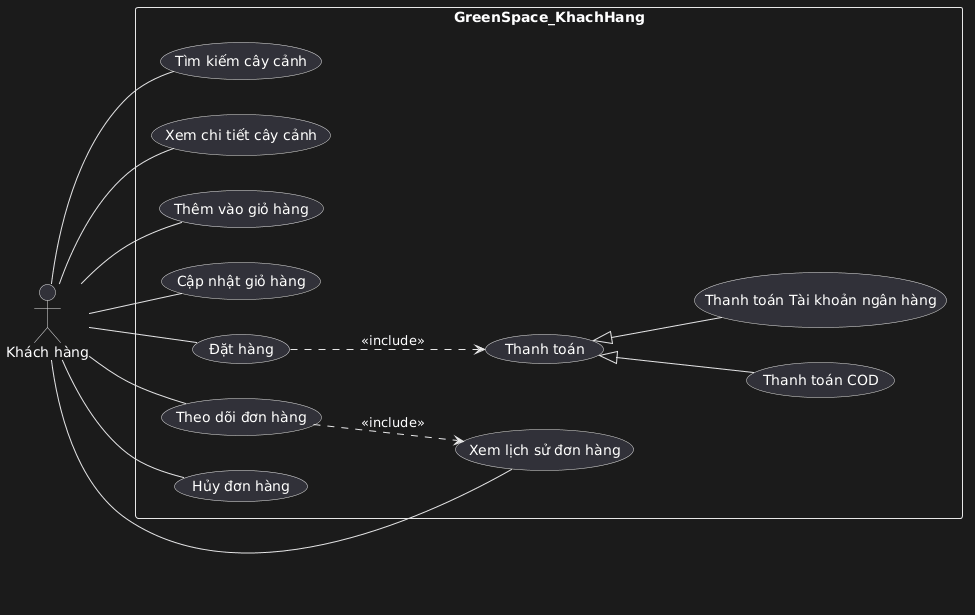
\includegraphics[width=0.85\textwidth]{KhachHangUsecase.png}
    \caption{\textit{Sơ đồ Use Case của tác nhân Khách hàng}}
    \label{fig:usecase_khachhang}
\end{figure}

\textbf{2. Sơ đồ Use Case Quản trị viên (Admin)}

\begin{figure}[H]
    \centering
    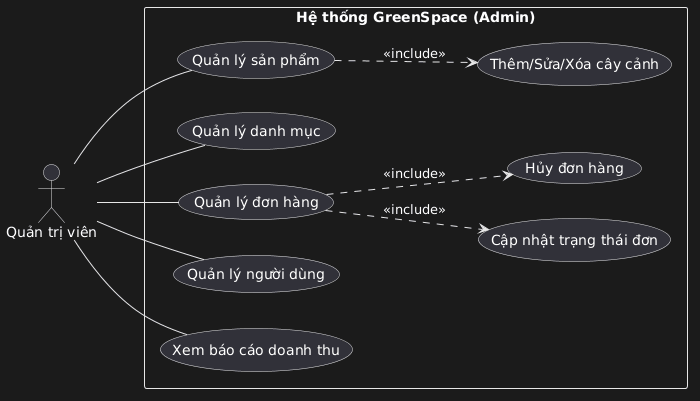
\includegraphics[width=0.85\textwidth]{AdminUsecase.png}
    \caption{\textit{Sơ đồ Use Case của tác nhân Quản trị viên}}
    \label{fig:usecase_admin}
\end{figure}

% ================================================================
% ĐẶC TẢ USE CASE CHI TIẾT - CHƯƠNG 3
% ================================================================
\subsection{Đặc tả Use Case chi tiết}

Phần này trình bày đặc tả chi tiết cho mười Use Case trọng yếu của hệ thống GreenSpace, bao gồm cả luồng chính (main flow) và các luồng thay thế (alternative flows) để phản ánh đầy đủ các tình huống có thể xảy ra trong thực tế vận hành.

% ----------------------------------------------------------------
\subsubsection{Use Case UC-01: Đăng ký tài khoản}

\begin{table}[H]
    \centering
    \caption{\textit{Đặc tả Use Case UC-01 --- Đăng ký tài khoản}}
    \vspace{0.2cm}
    \begin{tabularx}{\linewidth}{|>{\raggedright\arraybackslash}p{3.5cm}|Y|}
        \hline
        \textbf{Thuộc tính} & \textbf{Nội dung} \\ \hline
        Mã Use Case & UC-01 \\ \hline
        Tên & Đăng ký tài khoản \\ \hline
        Tác nhân chính & Khách hàng (người dùng chưa có tài khoản) \\ \hline
        Mô tả & Cho phép người dùng mới tạo tài khoản trên hệ thống GreenSpace để có thể đặt hàng, lưu địa chỉ giao hàng và theo dõi lịch sử mua hàng. \\ \hline
        Tiền điều kiện & Người dùng chưa đăng nhập. Trình duyệt có kết nối Internet. \\ \hline
        Hậu điều kiện & Tài khoản mới được tạo thành công trong bảng \texttt{users} với role = 'user' và status = 1. Người dùng được chuyển hướng đến trang chủ hoặc trang họ muốn truy cập. \\ \hline
        \textbf{Luồng chính} & \textbf{Các bước thực thi} \\ \hline
        & 1. Người dùng truy cập trang đăng ký (\texttt{/dang-ky}). \newline
          2. Hệ thống hiển thị form đăng ký gồm các trường: Họ tên, Email, Tên đăng nhập, Mật khẩu, Xác nhận mật khẩu. \newline
          3. Người dùng điền đầy đủ thông tin và nhấn ``Đăng ký''. \newline
          4. JavaScript kiểm tra phía client: định dạng email hợp lệ, mật khẩu $\geq$ 6 ký tự, hai trường mật khẩu khớp nhau. \newline
          5. Dữ liệu được gửi lên server (\texttt{POST /dang-ky}). \newline
          6. \texttt{AuthController} gọi \texttt{UserModel} kiểm tra email và username chưa tồn tại trong cơ sở dữ liệu. \newline
          7. Hệ thống băm mật khẩu bằng \texttt{password\_hash()} với thuật toán bcrypt. \newline
          8. Hệ thống chèn bản ghi mới vào bảng \texttt{users}. \newline
          9. Hệ thống tạo phiên đăng nhập tự động và chuyển hướng người dùng về trang chủ với thông báo ``Đăng ký thành công. Chào mừng bạn đến với GreenSpace!''. \\ \hline
        \textbf{Luồng thay thế} & \textbf{Các tình huống ngoại lệ} \\ \hline
        & \textbf{A1 --- Email đã tồn tại:} Tại bước 6, nếu email đã được đăng ký, hệ thống trả về thông báo lỗi ``Email này đã được sử dụng. Vui lòng dùng email khác hoặc đăng nhập.'' và giữ nguyên các giá trị đã nhập. \newline
          \textbf{A2 --- Username đã tồn tại:} Tại bước 6, nếu tên đăng nhập đã có người dùng, hệ thống hiển thị lỗi ``Tên đăng nhập này đã được sử dụng. Vui lòng chọn tên khác.''. \newline
          \textbf{A3 --- Mật khẩu không khớp:} Tại bước 4, nếu hai trường mật khẩu không giống nhau, JavaScript hiển thị lỗi inline ``Mật khẩu xác nhận không khớp'' ngay bên dưới trường nhập liệu. \newline
          \textbf{A4 --- Lỗi cơ sở dữ liệu:} Tại bước 8, nếu có lỗi INSERT, hệ thống hiển thị thông báo ``Đã xảy ra lỗi hệ thống. Vui lòng thử lại sau.'' và ghi log lỗi. \\ \hline
    \end{tabularx}
\end{table}

% ----------------------------------------------------------------
% ----------------------------------------------------------------
\subsubsection{Use Case UC-02: Đăng nhập tài khoản}

\begin{table}[H]
    \centering
    \caption{\textit{Đặc tả Use Case UC-02 --- Đăng nhập tài khoản}}
    \vspace{0.2cm}
    \begin{tabularx}{\linewidth}{|>{\raggedright\arraybackslash}p{3.5cm}|Y|}
        \hline
        \textbf{Thuộc tính} & \textbf{Nội dung} \\ \hline
        Mã Use Case & UC-02 \\ \hline
        Tên & Đăng nhập tài khoản \\ \hline
        Tác nhân chính & Khách hàng hoặc Quản trị viên \\ \hline
        Mô tả & Cho phép người dùng đã có tài khoản xác thực danh tính và truy cập vào các tính năng yêu cầu đăng nhập như đặt hàng, xem lịch sử mua hàng và quản trị hệ thống. \\ \hline
        Tiền điều kiện & Người dùng đã có tài khoản hợp lệ và chưa đăng nhập. \\ \hline
        Hậu điều kiện & Phiên đăng nhập (Session) được tạo với đầy đủ thông tin người dùng. \\ \hline
        \textbf{Luồng chính} & \textbf{Các bước thực thi} \\ \hline
        & 1. Người dùng truy cập trang đăng nhập (\texttt{/dang-nhap}) hoặc bị chuyển hướng tự động khi cố truy cập trang bảo mật. \newline
          2. Hệ thống hiển thị form gồm: Email (hoặc tên đăng nhập) và Mật khẩu. \newline
          3. Người dùng nhập thông tin và nhấn ``Đăng nhập''. \newline
          4. Dữ liệu được gửi lên server (\texttt{POST /dang-nhap}). \newline
          5. \texttt{AuthController} gọi \texttt{UserModel::findByEmail()} để tìm bản ghi tương ứng. \newline
          6. Hệ thống gọi \texttt{password\_verify()} để kiểm tra mật khẩu với giá trị băm trong cơ sở dữ liệu. \newline
          7. Hệ thống gọi \texttt{session\_regenerate\_id(true)} để tái tạo Session ID, chống tấn công Session Fixation. \newline
          8. Lưu thông tin người dùng (id, email, full\_name, role) vào \texttt{\$\_SESSION}. \newline
          9. Nếu role = 'admin', chuyển hướng đến \texttt{/admin/dashboard}; ngược lại, chuyển về trang chủ. \\ \hline
        \textbf{Luồng thay thế} & \textbf{Các tình huống ngoại lệ} \\ \hline
        & \textbf{A1 --- Email không tồn tại hoặc mật khẩu sai:} Tại bước 5 hoặc 6, nếu dữ liệu không khớp, hệ thống hiển thị lỗi chung ``Email hoặc mật khẩu không đúng.'' (không chỉ rõ lỗi nào để tránh lộ thông tin). \newline
          \textbf{A2 --- Quên mật khẩu:} Người dùng nhấn vào liên kết ``Quên mật khẩu?'' và được chuyển đến trang hướng dẫn khôi phục. \\ \hline
    \end{tabularx}
\end{table}

% ----------------------------------------------------------------
\subsubsection{Use Case UC-03: Thêm sản phẩm vào giỏ hàng}

\begin{table}[H]
    \centering
    \caption{\textit{Đặc tả Use Case UC-03 --- Thêm sản phẩm vào giỏ hàng}}
    \vspace{0.2cm}
    \begin{tabularx}{\linewidth}{|>{\raggedright\arraybackslash}p{3.5cm}|Y|}
        \hline
        \textbf{Thuộc tính} & \textbf{Nội dung} \\ \hline
        Mã Use Case & UC-03 \\ \hline
        Tên & Thêm sản phẩm vào giỏ hàng \\ \hline
        Tác nhân chính & Khách hàng (đã hoặc chưa đăng nhập) \\ \hline
        Mô tả & Cho phép khách hàng thêm một sản phẩm với số lượng mong muốn vào giỏ hàng của mình thông qua cơ chế AJAX không tải lại trang. \\ \hline
        Tiền điều kiện & Sản phẩm tồn tại và đang ở trạng thái active (status = 1). Số lượng tồn kho $\geq$ 1. \\ \hline
        Hậu điều kiện & Bản ghi trong bảng \texttt{cart} được tạo mới hoặc cập nhật số lượng. Badge số lượng giỏ hàng trên header được cập nhật. Toast notification xuất hiện xác nhận. \\ \hline
        \textbf{Luồng chính} & \textbf{Các bước thực thi} \\ \hline
        & 1. Khách hàng đang xem trang danh sách hoặc trang chi tiết sản phẩm. \newline
          2. Khách hàng chọn số lượng (mặc định là 1) và nhấn nút ``Thêm vào giỏ'' hoặc biểu tượng giỏ hàng. \newline
          3. JavaScript gửi AJAX POST request đến \texttt{/gio-hang/them} với payload JSON gồm \texttt{product\_id}, \texttt{variant\_id} (nếu có) và \texttt{quantity}. \newline
          4. \texttt{CartController} kiểm tra xem người dùng đã đăng nhập chưa (thông qua Session); nếu chưa, lấy guest\_id từ cookie hoặc tạo mới. \newline
          5. \texttt{CartController} gọi \texttt{CartService::addItem()} để xử lý. \newline
          6. \texttt{CartService} gọi \texttt{ProductModel::findById()} để lấy thông tin sản phẩm và kiểm tra tồn kho. \newline
          7. \texttt{CartService} kiểm tra xem sản phẩm đã có trong giỏ hàng chưa. \newline
          8a. Nếu chưa có: thêm bản ghi mới vào bảng \texttt{cart}. \newline
          8b. Nếu đã có: cập nhật trường \texttt{quantity} (cộng thêm số lượng yêu cầu). \newline
          9. Server trả về JSON: \texttt{\{success: true, cart\_count: N, message: "Đã thêm vào giỏ hàng"\}}. \newline
          10. JavaScript cập nhật badge số lượng trên header và hiển thị toast notification màu xanh trong 3 giây. \\ \hline
        \textbf{Luồng thay thế} & \textbf{Các tình huống ngoại lệ} \\ \hline
        & \textbf{A1 --- Vượt quá tồn kho:} Tại bước 6, nếu số lượng yêu cầu > tồn kho hiện tại, server trả về \texttt{\{success: false, message: "Chỉ còn X sản phẩm trong kho"\}}. Toast màu đỏ hiển thị thông báo tương ứng. \newline
          \textbf{A2 --- Sản phẩm hết hàng:} Nếu tồn kho = 0, nút ``Thêm vào giỏ'' bị vô hiệu hóa và hiển thị trạng thái ``Hết hàng'' ngay trên trang sản phẩm. \newline
          \textbf{A3 --- Lỗi mạng:} Nếu AJAX request thất bại (timeout, mất kết nối), JavaScript hiển thị toast lỗi ``Không thể kết nối đến máy chủ. Vui lòng thử lại.''. \\ \hline
    \end{tabularx}
\end{table}
% ----------------------------------------------------------------
\subsubsection{Use Case UC-04: Thanh toán đặt hàng (Checkout)}

\begin{table}[H]
    \centering
    \caption{\textit{Đặc tả Use Case UC-04 --- Thanh toán đặt hàng}}
    \vspace{0.2cm}
    \small
    \begin{tabularx}{\linewidth}{|>{\raggedright\arraybackslash}p{3.5cm}|Y|}
        \hline
        \textbf{Thuộc tính} & \textbf{Nội dung} \\ \hline
        Mã Use Case & UC-04 \\ \hline
        Tên & Thanh toán đặt hàng (Checkout) \\ \hline
        Tác nhân chính & Khách hàng (đã đăng nhập) \\ \hline
        Mô tả & Cho phép khách hàng hoàn tất quy trình mua hàng bằng cách nhập thông tin giao hàng, chọn phương thức thanh toán và xác nhận đơn hàng. Hệ thống đảm bảo tính toàn vẹn dữ liệu thông qua PDO Transaction. \\ \hline
        Tiền điều kiện & Khách hàng đã đăng nhập. Giỏ hàng có ít nhất một sản phẩm. Tất cả sản phẩm trong giỏ hàng còn tồn kho. \\ \hline
        Hậu điều kiện & Đơn hàng được tạo trong bảng \texttt{orders}. Chi tiết đơn hàng được lưu trong \texttt{order\_details}. Tồn kho được trừ và ghi vào \texttt{inventory\_logs}. Bản ghi thanh toán được tạo trong \texttt{payments}. Giỏ hàng bị xóa. \\ \hline
        \textbf{Luồng chính} & \textbf{Các bước thực thi} \\ \hline
        & 1. Từ trang giỏ hàng, khách hàng nhấn ``Tiến hành thanh toán''. \newline
          2. Hệ thống kiểm tra trạng thái đăng nhập; nếu chưa đăng nhập, chuyển hướng đến trang đăng nhập và lưu URL để quay lại. \newline
          3. \texttt{CheckoutController} gọi \texttt{CartService::getSummary()} để lấy danh sách sản phẩm, tổng tiền, phí ship và giảm giá. \newline
          4. Hệ thống hiển thị trang checkout ba bước: (a) Chọn địa chỉ từ sổ hoặc nhập mới; (b) Thông tin người nhận; (c) Chọn phương thức thanh toán và tóm tắt đơn hàng. \newline
          5. Khách hàng điền/chọn thông tin và nhấn ``Đặt hàng''. \newline
          6. Server nhận POST request, \texttt{CheckoutController} khởi tạo \texttt{CheckoutService::processOrder()}. \newline
          7. \texttt{CheckoutService} thực thi PDO Transaction bao gồm các bước: (1) Validate Input, (2) Stock Check, (3) Get Summary, (4) User Update, (5) Address Management, (6) Tạo Order Header, (7) Lưu Order Details + ghi inventory\_logs, (8) Tạo Payment Record, (9) Xóa Cart. \newline
          8. \texttt{\$pdo->commit()} được gọi khi tất cả bước thành công. \newline
          9. Hệ thống chuyển hướng đến trang xác nhận hiển thị mã đơn hàng và thông tin tóm tắt. \\ \hline
        \textbf{Luồng thay thế} & \textbf{Các tình huống ngoại lệ} \\ \hline
        & \textbf{A1 --- Sản phẩm hết hàng khi kiểm tra:} Tại bước (2) của Transaction, nếu tồn kho của bất kỳ sản phẩm nào không đủ, \texttt{rollBack()} được gọi và hệ thống thông báo cụ thể sản phẩm nào đã hết hàng. \newline
          \textbf{A2 --- Giỏ hàng rỗng:} Tại bước 3, nếu giỏ hàng không có sản phẩm, hệ thống chuyển hướng về trang giỏ hàng với thông báo. \newline
          \textbf{A3 --- Lỗi cơ sở dữ liệu trong Transaction:} Bất kỳ exception nào trong khối try-catch đều kích hoạt \texttt{rollBack()}, đảm bảo không có dữ liệu không nhất quán. \newline
          \textbf{A4 --- Mã giảm giá không hợp lệ:} Nếu coupon đã hết hạn hoặc đã đạt giới hạn sử dụng, hệ thống thông báo và tiến hành thanh toán với giá gốc. \\ \hline
    \end{tabularx}
\end{table}

% ----------------------------------------------------------------
\subsubsection{Use Case UC-05: Quản lý sản phẩm (Admin)}

\begin{table}[H]
    \centering
    \caption{\textit{\u0110ặc tả Use Case UC-05 --- Quản lý sản phẩm}}
    \vspace{0.2cm}
    \begin{tabularx}{\linewidth}{|>{\raggedright\arraybackslash}p{3.5cm}|Y|}
        \hline
        \textbf{Thuộc tính} & \textbf{Nội dung} \\ \hline
        Mã Use Case & UC-05 \\ \hline
        Tên & Quản lý sản phẩm \\ \hline
        Tác nhân chính & Quản trị viên (Admin) \\ \hline
        Mô tả & Cho phép admin thực hiện đầy đủ các thao tác CRUD (Create, Read, Update, Delete) trên danh sách sản phẩm cây cảnh, bao gồm quản lý hình ảnh và biến thể sản phẩm. \\ \hline
        Tiền điều kiện & Admin đã đăng nhập với role = 'admin'. \\ \hline
        Hậu điều kiện & Dữ liệu sản phẩm trong bảng \texttt{products}, \texttt{product\_images} và \texttt{product\_variants} được cập nhật tương ứng với thao tác thực hiện. \\ \hline
        \textbf{Luồng chính (Thêm sản phẩm mới)} & \textbf{Các bước thực thi} \\ \hline
        & 1. Admin truy cập \texttt{/admin/san-pham} và nhấn ``Thêm sản phẩm mới''. \newline
          2. Hệ thống hiển thị form với các trường: Tên sản phẩm, Danh mục, Mô tả, Giá gốc, Giá khuyến mãi, Tồn kho, Mức độ chăm sóc (easy/medium/hard), Nhu cầu nước (low/medium/high), Upload ảnh đại diện, Upload ảnh phụ. \newline
          3. Admin điền thông tin và nhấn ``Lưu sản phẩm''. \newline
          4. Server nhận POST request, validate dữ liệu (tên không rỗng, giá > 0, tồn kho $\geq$ 0). \newline
          5. Hệ thống tự động sinh slug từ tên sản phẩm (chuyển về chữ thường, thay dấu cách bằng gạch ngang, loại bỏ ký tự đặc biệt). \newline
          6. Ảnh được upload, đổi tên thành timestamp để tránh trùng lặp, lưu vào thư mục \texttt{/public/uploads/products/}. \newline
          7. Bản ghi mới được INSERT vào bảng \texttt{products}. \newline
          8. Các ảnh phụ (nếu có) được INSERT vào bảng \texttt{product\_images}. \newline
          9. Hệ thống hiển thị thông báo ``Thêm sản phẩm thành công'' và quay về danh sách. \\ \hline
        \textbf{Luồng thay thế} & \textbf{Các tình huống ngoại lệ} \\ \hline
        & \textbf{A1 --- Tên sản phẩm trùng:} Hệ thống kiểm tra và thông báo nếu slug đã tồn tại, yêu cầu đổi tên. \newline
          \textbf{A2 --- File ảnh không hợp lệ:} Chỉ chấp nhận các định dạng jpg, jpeg, png, webp. Kích thước tối đa 5MB. \newline
          \textbf{A3 --- Xóa sản phẩm có đơn hàng liên quan:} Hệ thống không xóa vật lý mà chuyển \texttt{status = 0} (soft delete) để bảo toàn lịch sử đơn hàng. \\ \hline
    \end{tabularx}
\end{table}

% ----------------------------------------------------------------
\subsubsection{Use Case UC-06: Quản lý tồn kho và Nhật ký kho}

\begin{table}[H]
    \centering
    \caption{\textit{\u0110ặc tả Use Case UC-06 --- Quản lý tồn kho}}
    \vspace{0.2cm}
    \begin{tabularx}{\linewidth}{|>{\raggedright\arraybackslash}p{3.5cm}|Y|}
        \hline
        \textbf{Thuộc tính} & \textbf{Nội dung} \\ \hline
        Mã Use Case & UC-06 \\ \hline
        Tên & Quản lý tồn kho và xem nhật ký biến động kho \\ \hline
        Tác nhân chính & Quản trị viên (Admin) \\ \hline
        Mô tả & Hệ thống tự động ghi nhật ký mọi biến động tồn kho (nhập kho, xuất kho, hoàn kho) vào bảng \texttt{inventory\_logs} gắn liền với các đơn hàng cụ thể. Admin có thể xem lịch sử biến động để kiểm toán hàng hóa. \\ \hline
        Tiền điều kiện & Admin đã đăng nhập. \\ \hline
        Hậu điều kiện & Bảng \texttt{inventory\_logs} được cập nhật tự động khi có biến động kho. \\ \hline
        \textbf{Luồng chính} & \textbf{Các bước thực thi} \\ \hline
        & 1. \textbf{Khi admin duyệt đơn hàng:} \texttt{OrderController} gọi \texttt{InventoryService::deduct()} với thông tin sản phẩm và order\_id. Hệ thống trừ tồn kho trong bảng \texttt{products} và INSERT bản ghi \texttt{change\_type = 'deduct'} vào \texttt{inventory\_logs}. \newline
          2. \textbf{Khi admin hủy đơn hàng:} \texttt{OrderController} gọi \texttt{InventoryService::restore()} để hoàn lại tồn kho. Bản ghi \texttt{change\_type = 'restore'} được ghi vào \texttt{inventory\_logs}. \newline
          3. \textbf{Khi nhập hàng thủ công:} Admin truy cập trang quản lý sản phẩm, cập nhật tồn kho và hệ thống INSERT bản ghi \texttt{change\_type = 'import'} vào \texttt{inventory\_logs}. \newline
          4. Admin truy cập trang \texttt{/admin/inventory-logs} để xem toàn bộ nhật ký với thông tin: ID, Product ID, Order ID, Action, Quantity, Note, Created\_at. \\ \hline
        \textbf{Luồng thay thế} & \textbf{Các tình huống ngoại lệ} \\ \hline
        & \textbf{A1 --- Tồn kho âm:} Hệ thống có ràng buộc CHECK để ngăn tồn kho giảm xuống dưới 0. Nếu tồn kho không đủ để deduct, Transaction sẽ rollback và thông báo lỗi. \\ \hline
    \end{tabularx}
\end{table}

% ----------------------------------------------------------------
\subsubsection{Use Case UC-07: Theo dõi trạng thái đơn hàng}

\begin{table}[H]
    \centering
    \caption{\textit{\u0110ặc tả Use Case UC-07 --- Theo dõi trạng thái đơn hàng}}
    \vspace{0.2cm}
    \begin{tabularx}{\linewidth}{|>{\raggedright\arraybackslash}p{3.5cm}|Y|}
        \hline
        \textbf{Thuộc tính} & \textbf{Nội dung} \\ \hline
        Mã Use Case & UC-07 \\ \hline
        Tên & Theo dõi trạng thái đơn hàng \\ \hline
        Tác nhân chính & Khách hàng (đã đăng nhập) \\ \hline
        Mô tả & Cho phép khách hàng xem danh sách các đơn hàng đã đặt và theo dõi trạng thái xử lý hiện tại của từng đơn hàng. \\ \hline
        Tiền điều kiện & Khách hàng đã đăng nhập và đã có ít nhất một đơn hàng. \\ \hline
        Hậu điều kiện & Không thay đổi dữ liệu. Chỉ hiển thị thông tin. \\ \hline
        \textbf{Luồng chính} & \textbf{Các bước thực thi} \\ \hline
        & 1. Khách hàng truy cập trang hồ sơ cá nhân (\texttt{/tai-khoan}). \newline
          2. Hệ thống hiển thị khu vực ``Đơn hàng gần đây'' với 3 đơn mới nhất. \newline
          3. Khách hàng nhấn ``Xem tất cả'' để đến trang lịch sử đơn hàng đầy đủ. \newline
          4. Hệ thống lấy danh sách đơn hàng của user\_id đang đăng nhập từ bảng \texttt{orders}, sắp xếp theo created\_at giảm dần. \newline
          5. Mỗi đơn hàng hiển thị: Mã đơn, Ngày đặt, Tổng tiền, Trạng thái thanh toán (badge màu), Trạng thái đơn (badge màu), Nút ``Xem chi tiết''. \newline
          6. Khách hàng nhấn ``Xem chi tiết'' để xem danh sách sản phẩm trong đơn, địa chỉ giao hàng và lịch sử cập nhật trạng thái. \\ \hline
        \textbf{Luồng thay thế} & \textbf{Các tình huống ngoại lệ} \\ \hline
        & \textbf{A1 --- Chưa có đơn hàng nào:} Hệ thống hiển thị thông báo ``Bạn chưa có đơn hàng nào. Hãy khám phá các loại cây cảnh của chúng tôi!'' kèm nút ``Mua sắm ngay''. \\ \hline
    \end{tabularx}
\end{table}

% ----------------------------------------------------------------
% ----------------------------------------------------------------
\subsubsection{Use Case UC-08: Quản lý người dùng (Admin)}

\begin{table}[H]
    \centering
    \caption{\textit{\u0110ặc tả Use Case UC-08 --- Quản lý người dùng}}
    \vspace{0.2cm}
    \begin{tabularx}{\linewidth}{|>{\raggedright\arraybackslash}p{3.5cm}|Y|}
        \hline
        \textbf{Thuộc tính} & \textbf{Nội dung} \\ \hline
        Mã Use Case & UC-08 \\ \hline
        Tên & Quản lý người dùng \\ \hline
        Tác nhân chính & Quản trị viên (Admin) \\ \hline
        Mô tả & Cho phép admin xem danh sách toàn bộ tài khoản người dùng, tra cứu thông tin khách hàng và cấp/thu hồi quyền quản trị (role) của các tài khoản. \\ \hline
        Tiền điều kiện & Admin đã đăng nhập với role = 'admin'. \\ \hline
        Hậu điều kiện & (Trường hợp có thao tác) Trường \texttt{role} trong bảng \texttt{users} được cập nhật. \\ \hline
        \textbf{Luồng chính} & \textbf{Các bước thực thi} \\ \hline
        & 1. Admin truy cập \texttt{/admin/nguoi-dung}. \newline
          2. Hệ thống truy vấn CSDL và hiển thị bảng danh sách người dùng với: ID, Họ tên, Email, Số điện thoại, Role (badge màu), Ngày tạo. \newline
          3. Admin nhập từ khóa vào thanh tìm kiếm để lọc người dùng theo tên hoặc email. \newline
          4. Để thay đổi quyền, Admin chọn phân quyền mới (\texttt{user} hoặc \texttt{admin}) từ dropdown tại cột Thao tác. \newline
          5. Hệ thống gửi request cập nhật trường \texttt{role} trong bảng \texttt{users} và hiển thị thông báo "Cập nhật quyền thành công". \\ \hline
        \textbf{Luồng thay thế} & \textbf{Các tình huống ngoại lệ} \\ \hline
        & \textbf{A1 --- Không tìm thấy dữ liệu:} Tại bước 3, nếu từ khóa không khớp với bất kỳ người dùng nào, hệ thống hiển thị thông báo "Không tìm thấy người dùng phù hợp với từ khóa.". \newline
          \textbf{A2 --- Hạ quyền Admin duy nhất:} Tại bước 4, hệ thống kiểm tra nếu tài khoản đang thao tác là Admin duy nhất còn lại của hệ thống thì chặn lệnh hạ quyền xuống 'user' (để tránh hệ thống mất quyền quản trị) và hiển thị thông báo lỗi. \\ \hline
    \end{tabularx}
\end{table}

% ----------------------------------------------------------------
\subsubsection{Use Case UC-09: Quản lý Mã giảm giá (Admin)}

\begin{table}[H]
    \centering
    \caption{\textit{\u0110ặc tả Use Case UC-09 --- Quản lý mã giảm giá}}
    \vspace{0.2cm}
    \begin{tabularx}{\linewidth}{|>{\raggedright\arraybackslash}p{3.5cm}|Y|}
        \hline
        \textbf{Thuộc tính} & \textbf{Nội dung} \\ \hline
        Mã Use Case & UC-09 \\ \hline
        Tên & Quản lý mã giảm giá (Coupon) \\ \hline
        Tác nhân chính & Quản trị viên (Admin) \\ \hline
        Mô tả & Cho phép admin tạo, chỉnh sửa và vô hiệu hóa các mã giảm giá. Hệ thống tự động kiểm tra điều kiện áp dụng và giới hạn sử dụng khi khách hàng nhập mã. \\ \hline
        Tiền điều kiện & Admin đã đăng nhập. \\ \hline
        Hậu điều kiện & Bản ghi trong bảng \texttt{coupons} được tạo mới hoặc cập nhật. \\ \hline
        \textbf{Luồng chính (Tạo coupon mới)} & \textbf{Các bước thực thi} \\ \hline
        & 1. Admin truy cập \texttt{/admin/coupon} và nhấn ``Tạo mã giảm giá''. \newline
          2. Hệ thống hiển thị form gồm: Mã coupon (code), Loại giảm giá (percent/fixed), Giá trị giảm, Đơn hàng tối thiểu, Giới hạn lượt dùng, Ngày hết hạn. \newline
          3. Admin điền thông tin và lưu. \newline
          4. Hệ thống kiểm tra mã coupon chưa tồn tại (UNIQUE trên trường code). \newline
          5. INSERT bản ghi mới vào bảng \texttt{coupons}. \newline
          6. \textbf{Khi khách hàng áp dụng mã:} \texttt{CartService} gọi \texttt{CouponModel::validate(\$code, \$user\_id, \$order\_amount)} để kiểm tra: mã tồn tại, chưa hết hạn, chưa đạt giới hạn lượt dùng tổng, người dùng chưa dùng mã này (kiểm tra \texttt{coupon\_usages}), giá trị đơn hàng đạt tối thiểu. \newline
          7. Nếu hợp lệ, trả về số tiền giảm và hiển thị trong tóm tắt đơn hàng. \\ \hline
        \textbf{Luồng thay thế} & \textbf{Các tình huống ngoại lệ} \\ \hline
        & \textbf{A1 --- Mã đã hết hạn:} Thông báo ``Mã giảm giá đã hết hạn sử dụng.''. \newline
          \textbf{A2 --- Đơn hàng không đủ giá trị tối thiểu:} Thông báo cụ thể ``Đơn hàng tối thiểu để dùng mã này là X đồng.''. \newline
          \textbf{A3 --- Người dùng đã dùng mã này rồi:} Thông báo ``Bạn đã sử dụng mã giảm giá này trước đó.''. \\ \hline
    \end{tabularx}
\end{table}

% ----------------------------------------------------------------
\subsubsection{Use Case UC-10: Cập nhật thông tin cá nhân}

\begin{table}[H]
    \centering
    \caption{\textit{\u0110ặc tả Use Case UC-10 --- Cập nhật thông tin cá nhân}}
    \vspace{0.2cm}
    \begin{tabularx}{\linewidth}{|>{\raggedright\arraybackslash}p{3.5cm}|Y|}
        \hline
        \textbf{Thuộc tính} & \textbf{Nội dung} \\ \hline
        Mã Use Case & UC-10 \\ \hline
        Tên & Cập nhật thông tin cá nhân và sổ địa chỉ \\ \hline
        Tác nhân chính & Khách hàng (đã đăng nhập) \\ \hline
        Mô tả & Cho phép khách hàng cập nhật thông tin hồ sơ (họ tên, số điện thoại) và quản lý sổ địa chỉ giao hàng (thêm, sửa, xóa, đặt mặc định). \\ \hline
        Tiền điều kiện & Khách hàng đã đăng nhập. \\ \hline
        Hậu điều kiện & Bản ghi trong bảng \texttt{users} được cập nhật. Bảng \texttt{addresses} được cập nhật theo thao tác quản lý địa chỉ. \\ \hline
        \textbf{Luồng chính} & \textbf{Các bước thực thi} \\ \hline
        & 1. Khách hàng truy cập trang hồ sơ (\texttt{/tai-khoan}). \newline
          2. Hệ thống hiển thị form thông tin cá nhân với các trường đã điền sẵn từ CSDL: Họ tên, Email (chỉ đọc), Số điện thoại. \newline
          3. Khách hàng chỉnh sửa và nhấn ``Lưu thông tin''. \newline
          4. Server validate và UPDATE bảng \texttt{users}. Session được cập nhật để phản ánh tên mới. \newline
          5. \textbf{Thêm địa chỉ mới:} Khách hàng nhấn ``Thêm địa chỉ mới'', form inline xuất hiện. Điền thông tin và tích chọn ``Đặt làm địa chỉ mặc định'' (nếu muốn). \newline
          6. Server INSERT vào bảng \texttt{addresses}. Nếu is\_default = 1, tất cả địa chỉ khác của user được UPDATE về is\_default = 0 trong cùng Transaction. \newline
          7. \textbf{Xóa địa chỉ:} Khách hàng nhấn ``Xóa'' trên địa chỉ không phải mặc định. Confirm dialog xuất hiện. Sau khi xác nhận, bản ghi bị DELETE. \\ \hline
        \textbf{Luồng thay thế} & \textbf{Các tình huống ngoại lệ} \\ \hline
        & \textbf{A1 --- Xóa địa chỉ mặc định:} Không cho phép xóa địa chỉ đang là mặc định. Thông báo ``Vui lòng đặt địa chỉ khác làm mặc định trước khi xóa.''. \newline
          \textbf{A2 --- Số điện thoại không hợp lệ:} Validate định dạng số điện thoại Việt Nam (bắt đầu bằng 0, 10--11 chữ số). \\ \hline
    \end{tabularx}
\end{table}
\subsection{Thiết kế xử lý \& cấu trúc source}

\subsubsection{Mô hình MVC mở rộng}

Hệ thống GreenSpace được thiết kế theo mô hình kiến trúc \textbf{MVC (Model -- View -- Controller)} mở rộng, có bổ sung thêm \textbf{Service Layer} để xử lý các nghiệp vụ phức tạp.

Luồng xử lý tổng quát:
\begin{center}
\textbf{Client} $\rightarrow$ \textbf{Router} $\rightarrow$ \textbf{Controller} $\rightarrow$ \textbf{Service} $\rightarrow$ \textbf{Model} $\rightarrow$ \textbf{Database (MySQL)}
\end{center}

Vai trò của từng thành phần:
\begin{itemize}[leftmargin=*]
    \item \textbf{Model:} Tầng dữ liệu, tương tác trực tiếp với MySQL qua PDO. Ví dụ: \texttt{ProductModel} thực hiện các truy vấn lấy sản phẩm, tìm theo slug, cập nhật tồn kho.
    \item \textbf{View:} Tầng giao diện, hiển thị dữ liệu dưới dạng HTML/CSS. Các file template tổ chức trong \texttt{/views/} theo từng module.
    \item \textbf{Controller:} Tầng trung gian, tiếp nhận request, điều phối luồng dữ liệu thông qua các \texttt{Service} và trả về \texttt{Response}.
    \item \textbf{Service Layer:} Xử lý nghiệp vụ tập trung. \texttt{ProductService} lọc/phân trang sản phẩm; \texttt{CheckoutService} điều phối đặt hàng qua PDO Transaction; \texttt{CartService} tính toán giỏ hàng.
    \item \textbf{Presenter \& DTO:} Sử dụng \texttt{Presenter} (như \texttt{ProductPresenter}) để định dạng dữ liệu cho View và \texttt{DTO} (\texttt{ProductCatalogRequestData}) để đóng gói dữ liệu yêu cầu, giúp code sạch và dễ bảo trì hơn.
    \item \textbf{Router:} Lớp định tuyến tùy chỉnh, ánh xạ URL vào Controller/Method thông qua các \texttt{RouteRegistrar}.
\end{itemize}

\subsubsection{Công nghệ sử dụng}

\begin{table}[H]
    \centering
    \caption{\textit{Các công nghệ chính được sử dụng trong hệ thống GreenSpace}}
    \vspace{0.2cm}
    \begin{tabularx}{\linewidth}{|>{\raggedright\arraybackslash}p{2.5cm}
                                  |>{\centering\arraybackslash}p{2cm}
                                  |Y|}
        \hline
        \textbf{Công nghệ} & \textbf{Phiên bản} & \textbf{Mục đích \& Lý do lựa chọn} \\ \hline
        PHP & 8.3 & Ngôn ngữ Back-end chính; hỗ trợ PDO mạnh mẽ, kiểu dữ liệu nghiêm ngặt \\ \hline
        MySQL & 8.0 & CSDL quan hệ; phù hợp mô hình có nhiều khóa ngoại, hỗ trợ Transaction \\ \hline
        HTML5/CSS3 & --- & Xây dựng giao diện tầng View với Tailwind CSS (CDN) và Vanilla CSS \\ \hline
        JavaScript & --- & Xử lý client-side: giỏ hàng AJAX, xác thực form, toast thông báo \\ \hline
        Docker & --- & Container hóa môi trường với \texttt{Dockerfile} và \texttt{docker-compose.yml} ở gốc dự án \\ \hline
        Apache & --- & Web server; mod\_rewrite hỗ trợ Friendly URLs qua \texttt{.htaccess} \\ \hline
        PDO & --- & Truy cập CSDL trừu tượng; Prepared Statements chống SQL Injection \\ \hline
    \end{tabularx}
\end{table}

\subsection{Cấu trúc mã nguồn dự án}

\begin{itemize}[leftmargin=*]
    \item \textbf{/app} --- Logic xử lý cốt lõi:
    \begin{itemize}
        \item \texttt{/core}: Các lớp cơ sở như Router, Controller, Response.
        \item \texttt{/controllers}: Tiếp nhận HTTP request (ví dụ: \texttt{ProductController}, \texttt{AdminPageController}).
        \item \texttt{/services}: Chứa logic nghiệp vụ (ví dụ: \texttt{CheckoutService}, \texttt{CartService}).
        \item \texttt{/models}: Định nghĩa cấu trúc dữ liệu và tương tác Database.
        \item \texttt{/presenters}: Định dạng dữ liệu trước khi đưa ra View.
        \item \texttt{/routing}: Đăng ký các tuyến đường (Route) cho hệ thống.
        \item \texttt{/views}: Template PHP hiển thị giao diện.
    \end{itemize}
    \item \textbf{/public} --- Điểm vào duy nhất (\texttt{index.php}), chứa file \texttt{.htaccess} điều hướng.
    \item \textbf{/config} --- Cấu hình hệ thống (\texttt{config.php}) và kết nối CSDL (\texttt{database.php}).
    \item \textbf{/tests} --- Các kịch bản kiểm thử tự động (\texttt{test\_db.php}, \texttt{test\_products.php}).
    \item \textbf{Gốc dự án} --- Chứa \texttt{Dockerfile}, \texttt{docker-compose.yml} và tài liệu hướng dẫn.
\end{itemize}

\subsection{Cơ chế điều hướng và Friendly URL}

\subsubsection{Router tùy chỉnh}

\begin{table}[H]
    \centering
    \caption{\textit{Ví dụ một số route tiêu biểu trong hệ thống}}
    \vspace{0.2cm}
    \begin{tabularx}{\linewidth}{|>{\raggedright\arraybackslash}p{4cm}
                                  |>{\raggedright\arraybackslash}p{5cm}
                                  |Y|}
        \hline
        \textbf{URL Pattern} & \textbf{Controller::Method} & \textbf{Mô tả} \\ \hline
        \texttt{/product/\{slug\}} & \texttt{ProductController::detail} & Chi tiết sản phẩm \\ \hline
        \texttt{/category/\{slug\}} & \texttt{ProductController::category} & Danh sách theo danh mục \\ \hline
        \texttt{/cart} & \texttt{CartController::index} & Trang giỏ hàng \\ \hline
        \texttt{/checkout} & \texttt{CheckoutController::index} & Trang thanh toán \\ \hline
        \texttt{/admin/orders} & \texttt{AdminPageController::orders} & Quản lý đơn hàng (admin) \\ \hline
    \end{tabularx}
\end{table}

\subsubsection{Cơ chế Slug và SEO}

Slug là chuỗi định danh thân thiện sinh tự động từ tên sản phẩm (ví dụ: \texttt{/san-pham/cay-luoi-ho}), mang lại hai lợi ích: URL chứa từ khóa giúp SEO tốt hơn và ẩn ID nội bộ khỏi người dùng bên ngoài.

\subsection{Quy trình nghiệp vụ}

\subsubsection{Quy trình mua hàng (dành cho Khách hàng)}

\begin{itemize}[leftmargin=*]
    \item \textbf{Bước 1 --- Tìm kiếm sản phẩm:} Khách hàng duyệt danh mục hoặc tìm kiếm theo từ khóa, lọc giá/danh mục/mức độ chăm sóc.
    \item \textbf{Bước 2 --- Xem chi tiết sản phẩm:} Xem hình ảnh, giá, hướng dẫn chăm sóc, chọn biến thể rồi ``Thêm vào giỏ hàng''.
    \item \textbf{Bước 3 --- Quản lý giỏ hàng:} Điều chỉnh số lượng, xóa sản phẩm; hệ thống cập nhật tổng tiền tức thì.
    \item \textbf{Bước 4 --- Xác thực đăng nhập:} Nếu chưa đăng nhập, hệ thống chuyển hướng rồi tự quay lại trang thanh toán.
    \item \textbf{Bước 5 --- Nhập thông tin và thanh toán:} Chọn địa chỉ từ sổ hoặc nhập mới; chọn phương thức COD hoặc chuyển khoản.
    \item \textbf{Bước 6 --- Xác nhận đơn hàng:} \texttt{CheckoutService} kiểm tra tồn kho, lưu đơn qua PDO Transaction và hiển thị mã đơn thành công.
\end{itemize}

\subsubsection{Quy trình quản lý đơn hàng (dành cho Quản trị viên)}

\begin{itemize}[leftmargin=*]
    \item \textbf{Bước 1:} Admin đăng nhập bằng tài khoản \texttt{role = admin}; hệ thống kiểm tra phiên và phân quyền.
    \item \textbf{Bước 2:} Truy cập ``Quản lý đơn hàng'', lọc theo trạng thái.
    \item \textbf{Bước 3:} Kiểm tra đơn hàng --- duyệt nếu hợp lệ, hủy nếu hết hàng/gian lận (hệ thống tự hoàn kho qua \texttt{inventory\_logs}).
    \item \textbf{Bước 4:} Cập nhật trạng thái thành ``Đã giao'' khi vận chuyển hoàn tất.
\end{itemize}

\subsection{Thiết kế cơ sở dữ liệu}

\subsubsection{Biểu đồ Thực thể Liên kết (ERD)}

\begin{figure}[H]
    \centering
    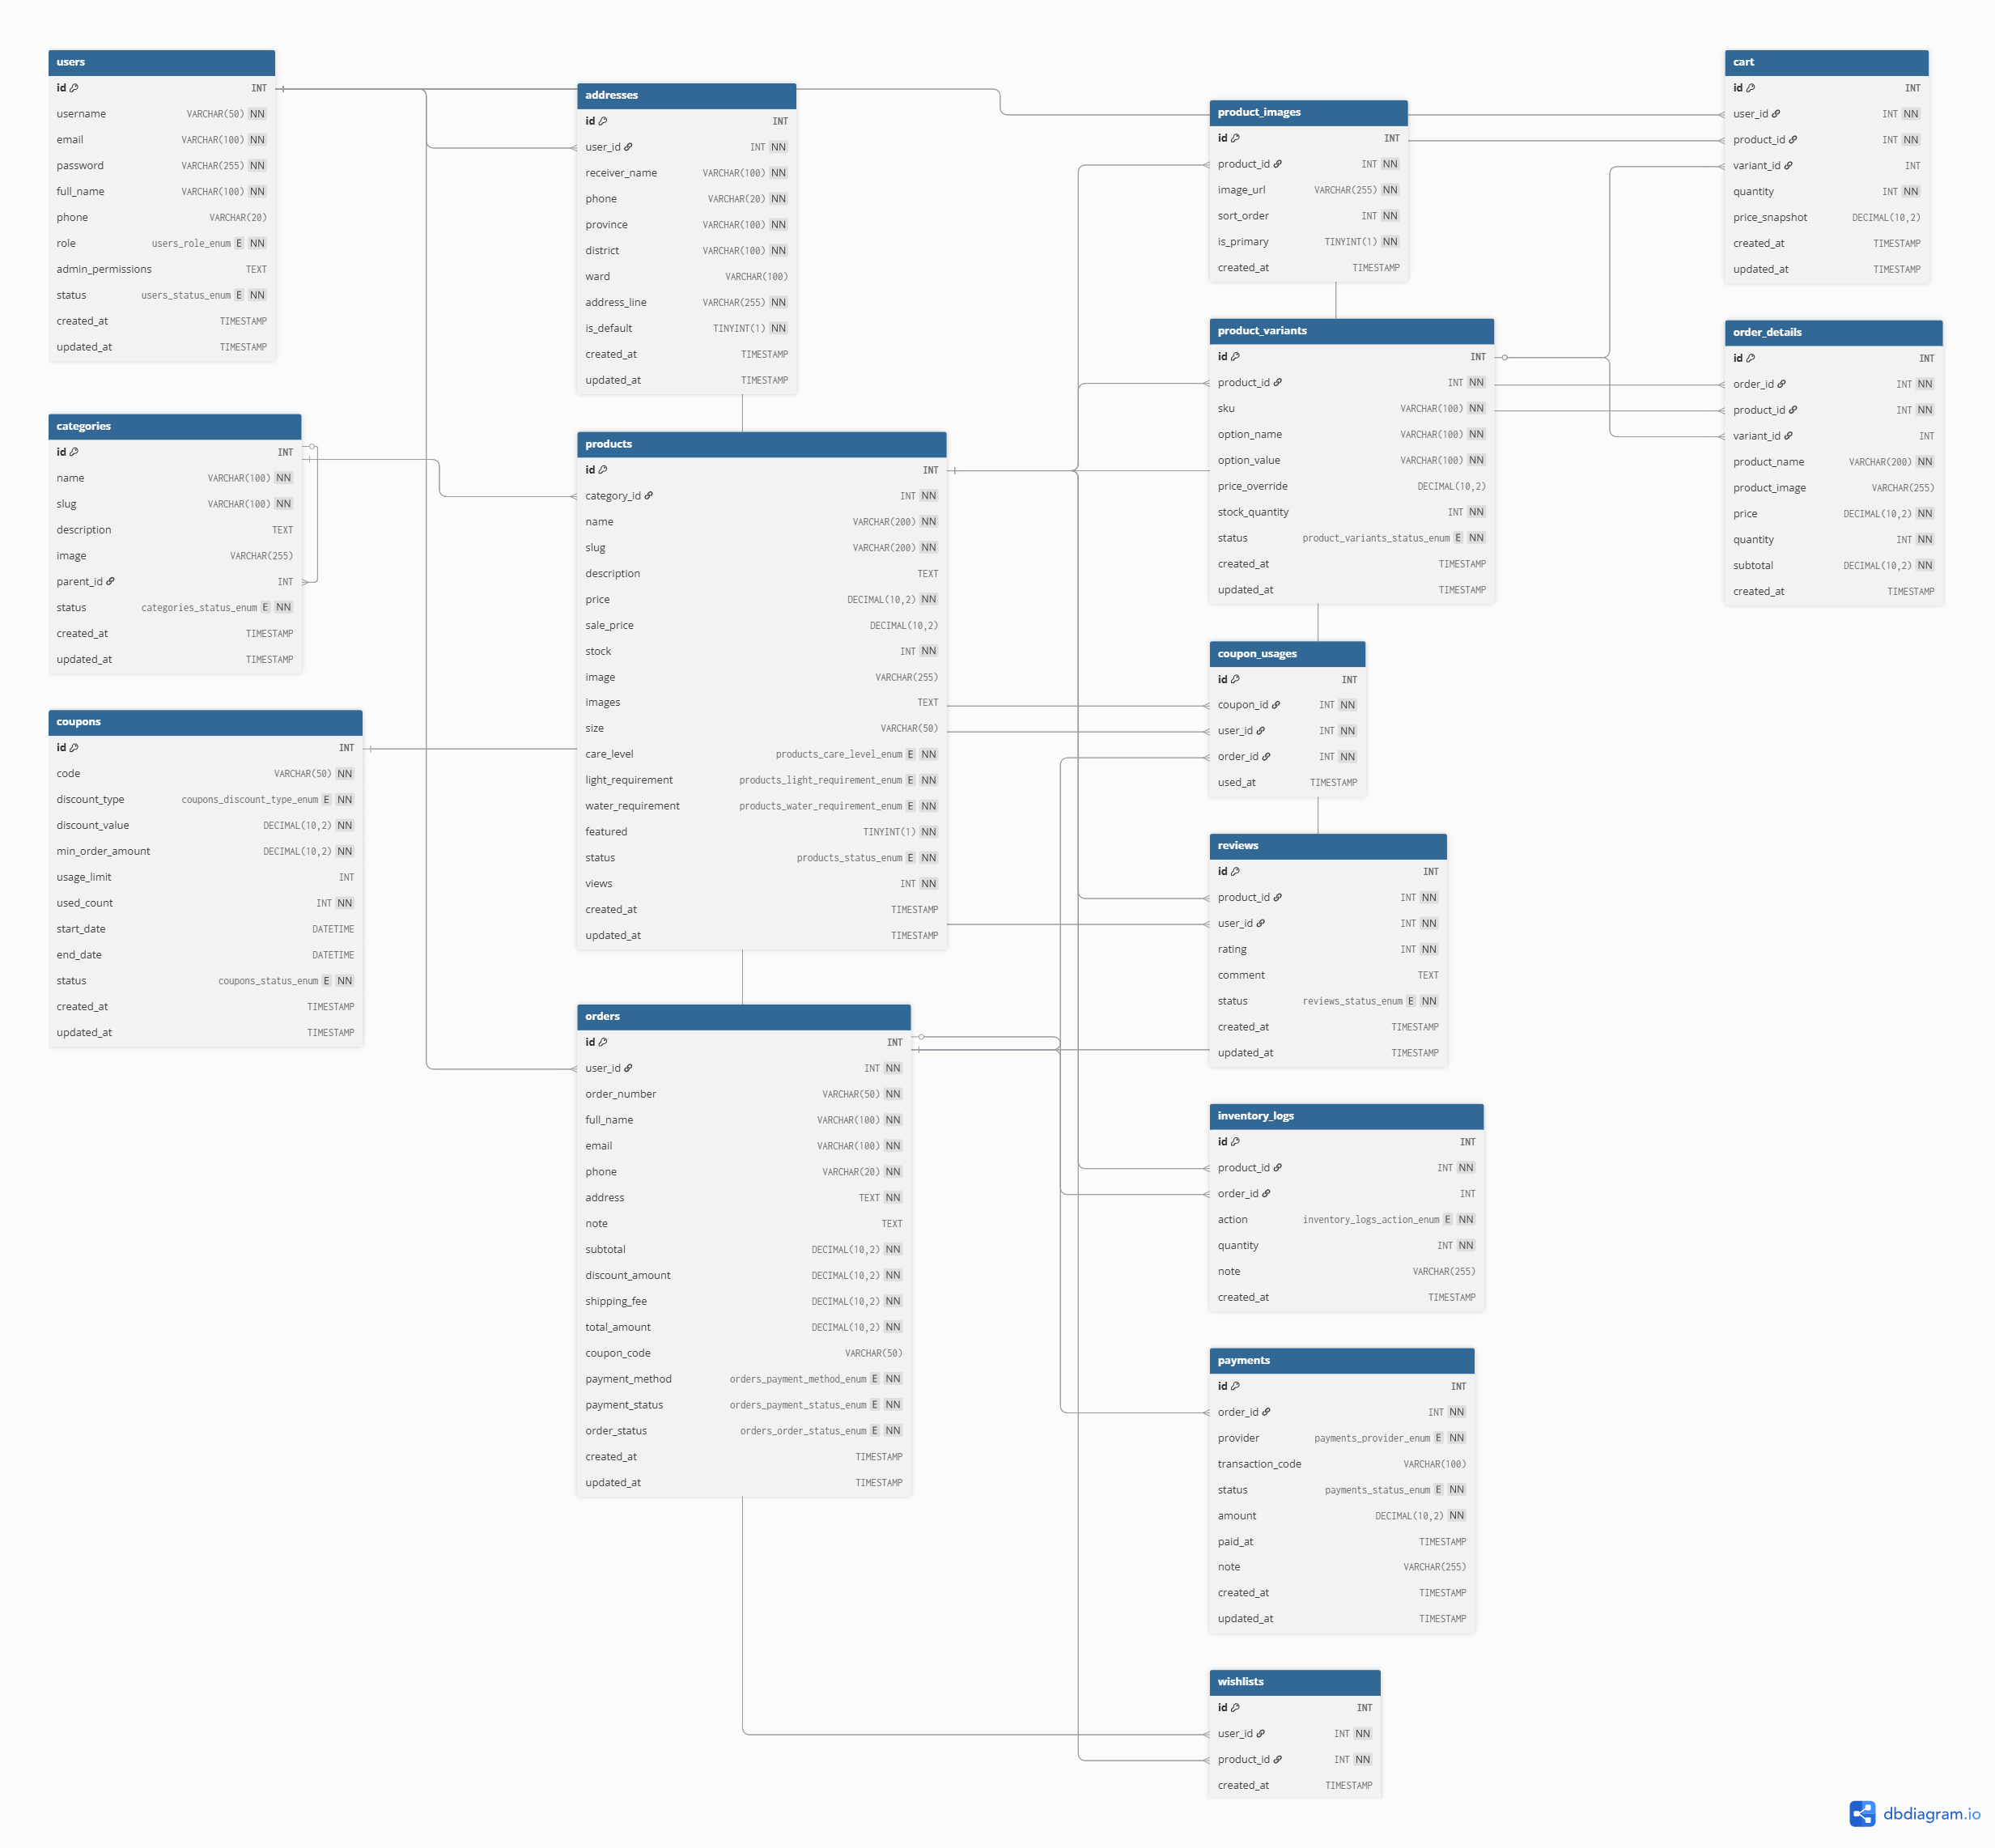
\includegraphics[width=\textwidth]{ERD_GreenSpace.png}
    \caption{\textit{Biểu đồ Thực thể Liên kết (ERD) chi tiết hệ thống GreenSpace}}
    \label{fig:erd_full}
\end{figure}

% ================================================================
% ĐẶC TẢ 16 BẢNG CƠ SỞ DỮ LIỆU - ĐÃ ĐỒNG BỘ SQL
% ================================================================

\subsubsection{Đặc tả chi tiết 16 bảng dữ liệu (Data Dictionary)}

Cơ sở dữ liệu của hệ thống WebGreenSpace được chuẩn hóa và chia thành 5 phân hệ cốt lõi. Cấu trúc bảng được thiết kế để đảm bảo tính toàn vẹn dữ liệu (Data Integrity) và kỹ thuật lưu vết (Snapshot) cho các giao dịch thương mại.

% ------------------------------------------------
\vspace{0.3cm}
\textbf{A. Phân hệ Quản lý Người dùng (User Management)}

\begin{table}[H]
    \centering
    \caption{\textit{Bảng 1: Đặc tả bảng \texttt{users} --- Quản lý tài khoản}}
    \vspace{0.2cm}
    \begin{tabularx}{\linewidth}{|>{\raggedright\arraybackslash}p{3cm}|l|l|Y|}
        \hline
        \textbf{Tên trường} & \textbf{Kiểu dữ liệu} & \textbf{Ràng buộc} & \textbf{Mô tả} \\ \hline
        \texttt{id} & INT & PK, AUTO\_INC & Khóa chính \\ \hline
        \texttt{username} & VARCHAR(50) & UNIQUE, NOT NULL & Tên đăng nhập \\ \hline
        \texttt{email} & VARCHAR(100) & UNIQUE, NOT NULL & Địa chỉ email \\ \hline
        \texttt{password} & VARCHAR(255) & NOT NULL & Mật khẩu (Mã hóa Bcrypt) \\ \hline
        \texttt{full\_name} & VARCHAR(100) & NOT NULL & Họ và tên đầy đủ \\ \hline
        \texttt{phone} & VARCHAR(20) & NULL & Số điện thoại \\ \hline
        \texttt{role} & ENUM & DEFAULT 'user' & Quyền: \texttt{admin}, \texttt{user} \\ \hline
        \texttt{admin\_perms}& TEXT & NULL & Phân quyền chi tiết cho Admin (JSON) \\ \hline
        \texttt{status} & ENUM & DEFAULT 'active' & Trạng thái: \texttt{active}, \texttt{inactive} \\ \hline
    \end{tabularx}
\end{table}

\begin{table}[H]
    \centering
    \caption{\textit{Bảng 2: Đặc tả bảng \texttt{addresses} --- Sổ địa chỉ giao hàng}}
    \vspace{0.2cm}
    \begin{tabularx}{\linewidth}{|>{\raggedright\arraybackslash}p{3cm}|l|l|Y|}
        \hline
        \textbf{Tên trường} & \textbf{Kiểu dữ liệu} & \textbf{Ràng buộc} & \textbf{Mô tả} \\ \hline
        \texttt{id} & INT & PK, AUTO\_INC & Khóa chính \\ \hline
        \texttt{user\_id} & INT & FK $\rightarrow$ users.id & Thuộc về khách hàng nào \\ \hline
        \texttt{receiver\_name} & VARCHAR(100) & NOT NULL & Tên người nhận hàng \\ \hline
        \texttt{phone} & VARCHAR(20) & NOT NULL & Số điện thoại người nhận \\ \hline
        \texttt{address\_line}& VARCHAR(255) & NOT NULL & Số nhà, tên đường chi tiết \\ \hline
        \texttt{ward} & VARCHAR(100) & NULL & Phường / Xã \\ \hline
        \texttt{district} & VARCHAR(100) & NOT NULL & Quận / Huyện \\ \hline
        \texttt{province} & VARCHAR(100) & NOT NULL & Tỉnh / Thành phố \\ \hline
        \texttt{is\_default} & TINYINT(1) & DEFAULT 0 & Đánh dấu địa chỉ mặc định (1=Có) \\ \hline
    \end{tabularx}
\end{table}

% ------------------------------------------------
\vspace{0.3cm}
\textbf{B. Phân hệ Danh mục và Sản phẩm (Catalog Management)}

\begin{table}[H]
    \centering
    \caption{\textit{Bảng 3: Đặc tả bảng \texttt{categories} --- Phân loại danh mục}}
    \vspace{0.2cm}
    \begin{tabularx}{\linewidth}{|>{\raggedright\arraybackslash}p{3cm}|l|l|Y|}
        \hline
        \textbf{Tên trường} & \textbf{Kiểu dữ liệu} & \textbf{Ràng buộc} & \textbf{Mô tả} \\ \hline
        \texttt{id} & INT & PK, AUTO\_INC & Khóa chính \\ \hline
        \texttt{parent\_id} & INT & FK $\rightarrow$ cat.id & Khóa ngoại đệ quy cho danh mục con \\ \hline
        \texttt{name} & VARCHAR(100) & NOT NULL & Tên danh mục \\ \hline
        \texttt{slug} & VARCHAR(100) & UNIQUE, NOT NULL & Đường dẫn URL thân thiện \\ \hline
        \texttt{image} & VARCHAR(255) & NULL & Ảnh đại diện danh mục \\ \hline
        \texttt{status} & ENUM & DEFAULT 'active' & Trạng thái: \texttt{active}, \texttt{inactive} \\ \hline
    \end{tabularx}
\end{table}

\begin{table}[H]
    \centering
    \caption{\textit{Bảng 4: Đặc tả bảng \texttt{products} --- Hồ sơ cây cảnh}}
    \vspace{0.2cm}
    \begin{tabularx}{\linewidth}{|>{\raggedright\arraybackslash}p{3.5cm}|l|l|Y|}
        \hline
        \textbf{Tên trường} & \textbf{Kiểu dữ liệu} & \textbf{Ràng buộc} & \textbf{Mô tả} \\ \hline
        \texttt{id} & INT & PK, AUTO\_INC & Khóa chính \\ \hline
        \texttt{category\_id} & INT & FK $\rightarrow$ cat.id & Thuộc danh mục nào \\ \hline
        \texttt{name} & VARCHAR(200) & NOT NULL & Tên cây cảnh \\ \hline
        \texttt{slug} & VARCHAR(200) & UNIQUE, NOT NULL & Đường dẫn URL sản phẩm \\ \hline
        \texttt{price} & DECIMAL(10,2) & NOT NULL & Giá bán niêm yết \\ \hline
        \texttt{sale\_price} & DECIMAL(10,2) & NULL & Giá khuyến mãi \\ \hline
        \texttt{stock} & INT & DEFAULT 0 & Số lượng tồn kho tổng \\ \hline
        \texttt{image} & VARCHAR(255) & NULL & Ảnh đại diện \\ \hline
        \texttt{images} & TEXT & NULL & Mảng JSON chứa các ảnh phụ \\ \hline
        \texttt{size} & VARCHAR(50) & NULL & Kích thước chậu cây \\ \hline
        \texttt{care\_level} & ENUM & DEFAULT 'medium' & Độ khó chăm sóc (\texttt{easy, medium, hard}) \\ \hline
        \texttt{light\_req} & ENUM & DEFAULT 'medium' & Nhu cầu ánh sáng (\texttt{low, medium, high}) \\ \hline
        \texttt{water\_req} & ENUM & DEFAULT 'medium' & Nhu cầu tưới nước (\texttt{low, medium, high}) \\ \hline
        \texttt{featured} & TINYINT(1) & DEFAULT 0 & Đánh dấu sản phẩm nổi bật \\ \hline
        \texttt{views} & INT & DEFAULT 0 & Lượt xem sản phẩm \\ \hline
        \texttt{status} & ENUM & DEFAULT 'active' & Trạng thái hoạt động \\ \hline
    \end{tabularx}
\end{table}

\begin{table}[H]
    \centering
    \caption{\textit{Bảng 5: Đặc tả bảng \texttt{product\_images} --- Thư viện ảnh phụ}}
    \vspace{0.2cm}
    \begin{tabularx}{\linewidth}{|>{\raggedright\arraybackslash}p{3cm}|l|l|Y|}
        \hline
        \textbf{Tên trường} & \textbf{Kiểu dữ liệu} & \textbf{Ràng buộc} & \textbf{Mô tả} \\ \hline
        \texttt{id} & INT & PK, AUTO\_INC & Khóa chính \\ \hline
        \texttt{product\_id} & INT & FK $\rightarrow$ products.id & Thuộc về sản phẩm nào \\ \hline
        \texttt{image\_url} & VARCHAR(255) & NOT NULL & Đường dẫn lưu ảnh \\ \hline
        \texttt{sort\_order} & INT & DEFAULT 0 & Thứ tự hiển thị \\ \hline
        \texttt{is\_primary} & TINYINT(1) & DEFAULT 0 & Cờ đánh dấu ảnh chính (1=Có) \\ \hline
    \end{tabularx}
\end{table}

\begin{table}[H]
    \centering
    \caption{\textit{Bảng 6: Đặc tả bảng \texttt{product\_variants} --- Biến thể sản phẩm}}
    \vspace{0.2cm}
    \begin{tabularx}{\linewidth}{|>{\raggedright\arraybackslash}p{3cm}|l|l|Y|}
        \hline
        \textbf{Tên trường} & \textbf{Kiểu dữ liệu} & \textbf{Ràng buộc} & \textbf{Mô tả} \\ \hline
        \texttt{id} & INT & PK, AUTO\_INC & Khóa chính \\ \hline
        \texttt{product\_id} & INT & FK $\rightarrow$ products.id & Liên kết với sản phẩm gốc \\ \hline
        \texttt{sku} & VARCHAR(100) & UNIQUE, NOT NULL & Mã quản lý hàng hóa (SKU) \\ \hline
        \texttt{option\_name} & VARCHAR(100) & NOT NULL & Tên thuộc tính (Vd: size, color) \\ \hline
        \texttt{option\_value}& VARCHAR(100) & NOT NULL & Giá trị thuộc tính (Vd: Lớn, Đỏ) \\ \hline
        \texttt{price\_override}& DECIMAL(10,2)& NULL & Giá ghi đè của biến thể này \\ \hline
        \texttt{stock\_quantity}& INT & DEFAULT 0 & Tồn kho riêng cho biến thể \\ \hline
    \end{tabularx}
\end{table}

% ------------------------------------------------
\vspace{0.3cm}
\textbf{C. Phân hệ Mua hàng và Thanh toán (Order \& Checkout)}

\begin{table}[H]
    \centering
    \caption{\textit{Bảng 7: Đặc tả bảng \texttt{cart} --- Giỏ hàng}}
    \vspace{0.2cm}
    \begin{tabularx}{\linewidth}{|>{\raggedright\arraybackslash}p{3cm}|l|l|Y|}
        \hline
        \textbf{Tên trường} & \textbf{Kiểu dữ liệu} & \textbf{Ràng buộc} & \textbf{Mô tả} \\ \hline
        \texttt{id} & INT & PK, AUTO\_INC & Khóa chính \\ \hline
        \texttt{user\_id} & INT & FK $\rightarrow$ users.id & Khách hàng \\ \hline
        \texttt{product\_id} & INT & FK $\rightarrow$ products.id & Sản phẩm \\ \hline
        \texttt{variant\_id} & INT & FK $\rightarrow$ variants.id& Biến thể (nếu có) \\ \hline
        \texttt{quantity} & INT & DEFAULT 1 & Số lượng \\ \hline
        \texttt{price\_snapshot}& DECIMAL(10,2)& NULL & Giá trị tạm tính tại thời điểm thêm \\ \hline
    \end{tabularx}
\end{table}

\begin{table}[H]
    \centering
    \caption{\textit{Bảng 8: Đặc tả bảng \texttt{orders} --- Phiếu đặt hàng}}
    \vspace{0.2cm}
    \begin{tabularx}{\linewidth}{|>{\raggedright\arraybackslash}p{3.5cm}|l|l|Y|}
        \hline
        \textbf{Tên trường} & \textbf{Kiểu dữ liệu} & \textbf{Ràng buộc} & \textbf{Mô tả} \\ \hline
        \texttt{id} & INT & PK, AUTO\_INC & Khóa chính \\ \hline
        \texttt{user\_id} & INT & FK $\rightarrow$ users.id & Người đặt hàng \\ \hline
        \texttt{order\_number} & VARCHAR(50) & UNIQUE, NOT NULL & Mã đơn hàng (Vd: ORD2026...) \\ \hline
        \texttt{full\_name} & VARCHAR(100) & NOT NULL & Tên người nhận (Snapshot) \\ \hline
        \texttt{email} & VARCHAR(100) & NOT NULL & Email liên hệ (Snapshot) \\ \hline
        \texttt{phone} & VARCHAR(20) & NOT NULL & Số điện thoại (Snapshot) \\ \hline
        \texttt{address} & TEXT & NOT NULL & Địa chỉ giao hàng đầy đủ \\ \hline
        \texttt{subtotal} & DECIMAL(10,2) & DEFAULT 0 & Tiền hàng trước giảm giá \\ \hline
        \texttt{discount\_amount}& DECIMAL(10,2)& DEFAULT 0 & Số tiền được giảm từ Coupon \\ \hline
        \texttt{shipping\_fee} & DECIMAL(10,2) & DEFAULT 0 & Phí vận chuyển \\ \hline
        \texttt{total\_amount} & DECIMAL(10,2) & NOT NULL & Tổng tiền phải thu cuối cùng \\ \hline
        \texttt{coupon\_code} & VARCHAR(50) & NULL & Mã giảm giá đã dùng \\ \hline
        \texttt{payment\_method}& ENUM & DEFAULT 'cod' & \texttt{cod}, \texttt{online\_mock} \\ \hline
        \texttt{payment\_status}& ENUM & DEFAULT 'unpaid' & \texttt{unpaid}, \texttt{pending\_review}, \texttt{paid}, \texttt{failed} \\ \hline
        \texttt{order\_status} & ENUM & DEFAULT 'pending' & \texttt{pending}, \texttt{confirmed}, \texttt{processing}... \\ \hline
    \end{tabularx}
\end{table}

\begin{table}[H]
    \centering
    \caption{\textit{Bảng 9: Đặc tả bảng \texttt{order\_details} --- Chi tiết mặt hàng trong đơn}}
    \vspace{0.2cm}
    \begin{tabularx}{\linewidth}{|>{\raggedright\arraybackslash}p{3cm}|l|l|Y|}
        \hline
        \textbf{Tên trường} & \textbf{Kiểu dữ liệu} & \textbf{Ràng buộc} & \textbf{Mô tả} \\ \hline
        \texttt{id} & INT & PK, AUTO\_INC & Khóa chính \\ \hline
        \texttt{order\_id} & INT & FK $\rightarrow$ orders.id & Thuộc đơn hàng \\ \hline
        \texttt{product\_id} & INT & FK $\rightarrow$ products.id & ID sản phẩm \\ \hline
        \texttt{product\_name} & VARCHAR(200) & NOT NULL & Tên SP tại thời điểm mua (Snapshot) \\ \hline
        \texttt{product\_image} & VARCHAR(255) & NULL & Ảnh SP tại thời điểm mua \\ \hline
        \texttt{price} & DECIMAL(10,2) & NOT NULL & Đơn giá chốt tại thời điểm mua \\ \hline
        \texttt{quantity} & INT & NOT NULL & Số lượng mua \\ \hline
        \texttt{subtotal} & DECIMAL(10,2) & NOT NULL & Thành tiền (\texttt{price} $\times$ \texttt{quantity}) \\ \hline
    \end{tabularx}
\end{table}

\begin{table}[H]
    \centering
    \caption{\textit{Bảng 10: Đặc tả bảng \texttt{payments} --- Giao dịch thanh toán}}
    \vspace{0.2cm}
    \begin{tabularx}{\linewidth}{|>{\raggedright\arraybackslash}p{3.5cm}|l|l|Y|}
        \hline
        \textbf{Tên trường} & \textbf{Kiểu dữ liệu} & \textbf{Ràng buộc} & \textbf{Mô tả} \\ \hline
        \texttt{id} & INT & PK, AUTO\_INC & Khóa chính \\ \hline
        \texttt{order\_id} & INT & FK $\rightarrow$ orders.id & Đơn hàng thanh toán \\ \hline
        \texttt{provider} & ENUM & DEFAULT 'cod' & Đơn vị cung cấp (\texttt{cod}, \texttt{online\_mock}) \\ \hline
        \texttt{transaction\_code}& VARCHAR(100) & NULL & Mã giao dịch trả về từ API \\ \hline
        \texttt{status} & ENUM & DEFAULT 'unpaid' & \texttt{unpaid}, \texttt{pending\_review}, \texttt{paid}, \texttt{failed} \\ \hline
        \texttt{amount} & DECIMAL(10,2) & NOT NULL & Số tiền giao dịch \\ \hline
        \texttt{paid\_at} & TIMESTAMP & NULL & Thời điểm xác nhận tiền vào \\ \hline
    \end{tabularx}
\end{table}

% ------------------------------------------------
\vspace{0.3cm}
\textbf{D. Phân hệ Tiếp thị và Tương tác (Marketing \& CRM)}

\begin{table}[H]
    \centering
    \caption{\textit{Bảng 11: Đặc tả bảng \texttt{coupons} --- Mã giảm giá}}
    \vspace{0.2cm}
    \begin{tabularx}{\linewidth}{|>{\raggedright\arraybackslash}p{3.5cm}|l|l|Y|}
        \hline
        \textbf{Tên trường} & \textbf{Kiểu dữ liệu} & \textbf{Ràng buộc} & \textbf{Mô tả} \\ \hline
        \texttt{id} & INT & PK, AUTO\_INC & Khóa chính \\ \hline
        \texttt{code} & VARCHAR(50) & UNIQUE, NOT NULL & Mã nhập (Vd: FREESHIP) \\ \hline
        \texttt{discount\_type} & ENUM & DEFAULT 'fixed' & Loại giảm (\texttt{fixed}, \texttt{percent}) \\ \hline
        \texttt{discount\_value}& DECIMAL(10,2) & NOT NULL & Mức giảm \\ \hline
        \texttt{min\_order\_amount}& DECIMAL(10,2)& DEFAULT 0 & Đơn hàng tối thiểu để áp dụng \\ \hline
        \texttt{usage\_limit} & INT & NULL & Tổng lượt sử dụng tối đa \\ \hline
        \texttt{used\_count} & INT & DEFAULT 0 & Số lượt đã sử dụng \\ \hline
        \texttt{start\_date} & DATETIME & NULL & Thời gian bắt đầu có hiệu lực \\ \hline
        \texttt{end\_date} & DATETIME & NULL & Thời gian hết hiệu lực \\ \hline
        \texttt{status} & ENUM & DEFAULT 'active' & \texttt{active}, \texttt{inactive} \\ \hline
    \end{tabularx}
\end{table}

\begin{table}[H]
    \centering
    \caption{\textit{Bảng 12: Đặc tả bảng \texttt{coupon\_usages} --- Lịch sử dùng mã}}
    \vspace{0.2cm}
    \begin{tabularx}{\linewidth}{|>{\raggedright\arraybackslash}p{3cm}|l|l|Y|}
        \hline
        \textbf{Tên trường} & \textbf{Kiểu dữ liệu} & \textbf{Ràng buộc} & \textbf{Mô tả} \\ \hline
        \texttt{id} & INT & PK, AUTO\_INC & Khóa chính \\ \hline
        \texttt{coupon\_id} & INT & FK $\rightarrow$ coupons.id & Mã giảm giá \\ \hline
        \texttt{user\_id} & INT & FK $\rightarrow$ users.id & Khách hàng \\ \hline
        \texttt{order\_id} & INT & FK $\rightarrow$ orders.id & Đơn hàng \\ \hline
        \texttt{used\_at} & TIMESTAMP & DEFAULT NOW() & Thời điểm dùng \\ \hline
    \end{tabularx}
\end{table}

\begin{table}[H]
    \centering
    \caption{\textit{Bảng 13: Đặc tả bảng \texttt{reviews} --- Đánh giá của khách hàng}}
    \vspace{0.2cm}
    \begin{tabularx}{\linewidth}{|>{\raggedright\arraybackslash}p{3cm}|l|l|Y|}
        \hline
        \textbf{Tên trường} & \textbf{Kiểu dữ liệu} & \textbf{Ràng buộc} & \textbf{Mô tả} \\ \hline
        \texttt{id} & INT & PK, AUTO\_INC & Khóa chính \\ \hline
        \texttt{product\_id} & INT & FK $\rightarrow$ products.id & Sản phẩm được đánh giá \\ \hline
        \texttt{user\_id} & INT & FK $\rightarrow$ users.id & Khách hàng viết \\ \hline
        \texttt{rating} & INT & CHECK (1-5) & Số sao (1 đến 5) \\ \hline
        \texttt{comment} & TEXT & NULL & Nội dung đánh giá \\ \hline
        \texttt{status} & ENUM & DEFAULT 'pending' & \texttt{pending}, \texttt{approved}, \texttt{rejected} \\ \hline
    \end{tabularx}
\end{table}

\begin{table}[H]
    \centering
    \caption{\textit{Bảng 14: Đặc tả bảng \texttt{wishlists} --- Danh mục yêu thích}}
    \vspace{0.2cm}
    \begin{tabularx}{\linewidth}{|>{\raggedright\arraybackslash}p{3cm}|l|l|Y|}
        \hline
        \textbf{Tên trường} & \textbf{Kiểu dữ liệu} & \textbf{Ràng buộc} & \textbf{Mô tả} \\ \hline
        \texttt{id} & INT & PK, AUTO\_INC & Khóa chính \\ \hline
        \texttt{user\_id} & INT & FK $\rightarrow$ users.id & Khách hàng \\ \hline
        \texttt{product\_id} & INT & FK $\rightarrow$ products.id & Sản phẩm \\ \hline
    \end{tabularx}
\end{table}

% ------------------------------------------------
\vspace{0.3cm}
\textbf{E. Phân hệ Vận hành và Hệ thống (Operations \& System)}

\begin{table}[H]
    \centering
    \caption{\textit{Bảng 15: Đặc tả bảng \texttt{inventory\_logs} --- Nhật ký biến động kho}}
    \vspace{0.2cm}
    \begin{tabularx}{\linewidth}{|>{\raggedright\arraybackslash}p{3cm}|l|l|Y|}
        \hline
        \textbf{Tên trường} & \textbf{Kiểu dữ liệu} & \textbf{Ràng buộc} & \textbf{Mô tả} \\ \hline
        \texttt{id} & INT & PK, AUTO\_INC & Khóa chính \\ \hline
        \texttt{product\_id} & INT & FK $\rightarrow$ products.id & Sản phẩm biến động kho \\ \hline
        \texttt{order\_id} & INT & FK $\rightarrow$ orders.id & Đơn hàng gây ra biến động (nếu có) \\ \hline
        \texttt{action} & ENUM & NOT NULL & Thao tác (\texttt{import}, \texttt{deduct}, \texttt{restore}, \texttt{adjust}) \\ \hline
        \texttt{quantity} & INT & NOT NULL & Số lượng biến động (LUÔN DƯƠNG) \\ \hline
        \texttt{note} & VARCHAR(255) & NULL & Lý do biến động \\ \hline
    \end{tabularx}
\end{table}

\begin{table}[H]
    \centering
    \caption{\textit{Bảng 16: Đặc tả bảng \texttt{admin\_notifications} --- Thông báo hệ thống (Bổ sung mở rộng)}}
    \vspace{0.2cm}
    \begin{tabularx}{\linewidth}{|>{\raggedright\arraybackslash}p{3cm}|l|l|Y|}
        \hline
        \textbf{Tên trường} & \textbf{Kiểu dữ liệu} & \textbf{Ràng buộc} & \textbf{Mô tả} \\ \hline
        \texttt{id} & INT & PK, AUTO\_INC & Khóa chính \\ \hline
        \texttt{title} & VARCHAR(150) & NOT NULL & Tiêu đề (Vd: Có đơn hàng mới) \\ \hline
        \texttt{message} & TEXT & NOT NULL & Nội dung chi tiết \\ \hline
        \texttt{type} & ENUM & NOT NULL & Phân loại (\texttt{new\_order}, \texttt{low\_stock}, \texttt{system}) \\ \hline
        \texttt{is\_read} & TINYINT(1) & DEFAULT 0 & Trạng thái đọc (0 = Chưa đọc, 1 = Đã đọc) \\ \hline
        \texttt{created\_at} & TIMESTAMP & DEFAULT NOW() & Thời điểm phát sinh thông báo \\ \hline
    \end{tabularx}
\end{table}

\subsection{Phân tích tính năng Sổ địa chỉ}

Bảng \texttt{addresses} liên kết với \texttt{users} qua \texttt{user\_id} theo quan hệ \textbf{1--N}: một người dùng có nhiều địa chỉ. Trường \texttt{is\_default} xác định địa chỉ mặc định. Khi thiết lập địa chỉ mới làm mặc định, \texttt{CheckoutService} cập nhật \texttt{is\_default = 0} cho tất cả địa chỉ còn lại trong cùng một Transaction, đảm bảo luôn chỉ có đúng một địa chỉ mặc định.

\subsection{Phân tích thuật toán Checkout và Tính toàn vẹn dữ liệu}

\subsubsection{Kỹ thuật PDO Transaction}

Hệ thống áp dụng Transaction của PDO theo nguyên tắc \textbf{Atomicity}: toàn bộ các bước đặt hàng là một đơn vị --- hoặc tất cả thành công (\texttt{commit()}), hoặc không ghi nhận gì (\texttt{rollBack()}).

\subsubsection{Quy trình xử lý chi tiết}

\begin{table}[H]
    \centering
    \caption{Các bước xử lý trong thuật toán Checkout}
    \vspace{0.2cm}
    \begin{tabularx}{\linewidth}{|>{\centering\arraybackslash}p{1cm}
                                  |>{\raggedright\arraybackslash}p{3cm}
                                  |Y|}
        \hline
        \textbf{Bước} & \textbf{Thao tác} & \textbf{Mục đích kỹ thuật} \\ \hline
        1 & Validate Input & Kiểm tra email, số điện thoại, địa chỉ; dùng Prepared Statements chống SQL Injection \\ \hline
        2 & Stock Check & Kiểm tra tồn kho từng sản phẩm; trả lỗi ngay nếu hết hàng \\ \hline
        3 & Get Summary & Lấy tổng tiền, phí ship, giảm giá từ \texttt{CartService} \\ \hline
        4 & User Update & Cập nhật \texttt{full\_name} và \texttt{phone} vào hồ sơ \\ \hline
        5 & Address Management & Lưu địa chỉ mới hoặc cập nhật \texttt{is\_default} \\ \hline
        6 & Order Header & Tạo bản ghi \texttt{orders}, sinh \texttt{order\_number} duy nhất \\ \hline
        7 & Order Details & Lưu từng sản phẩm vào \texttt{order\_details} với \texttt{price\_snapshot}; ghi \texttt{inventory\_logs} \\ \hline
        8 & Payment Record & Tạo bản ghi trong \texttt{payments} \\ \hline
        9 & Cart Cleanup & Xóa giỏ hàng sau khi đặt thành công \\ \hline
    \end{tabularx}
\end{table}

\subsection{Bảo mật hệ thống}

\begin{itemize}[leftmargin=*]
    \item \textbf{Băm mật khẩu:} Dùng \texttt{password\_hash()} với bcrypt; xác thực qua \texttt{password\_verify()}.
    \item \textbf{Session:} \texttt{session\_regenerate\_id(true)} sau đăng nhập để chống Session Fixation.
    \item \textbf{Phân quyền:} Mọi route admin kiểm tra \texttt{role = admin} trước khi thực thi.
    \item \textbf{Chống SQL Injection:} PDO Prepared Statements cho toàn bộ truy vấn.
    \item \textbf{Chống XSS:} \texttt{htmlspecialchars()} cho mọi dữ liệu đầu ra trong View.
\end{itemize}

\subsection{Sơ đồ Tuần tự (Sequence Diagram)}

\begin{figure}[H]
    \centering
    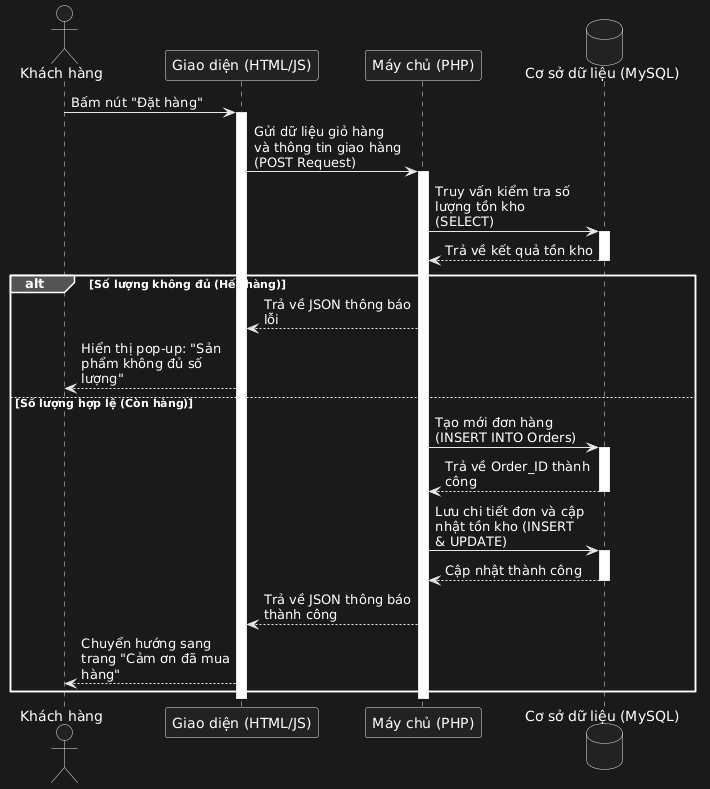
\includegraphics[width=0.9\textwidth]{SequenceDatHang.png}
    \caption{Sơ đồ tuần tự chức năng Đặt hàng}
    \label{fig:sequence_dathang}
\end{figure}

\subsection{Sơ đồ Hoạt động (Activity Diagram)}
\clearpage
\begin{figure}[H]
    \centering
    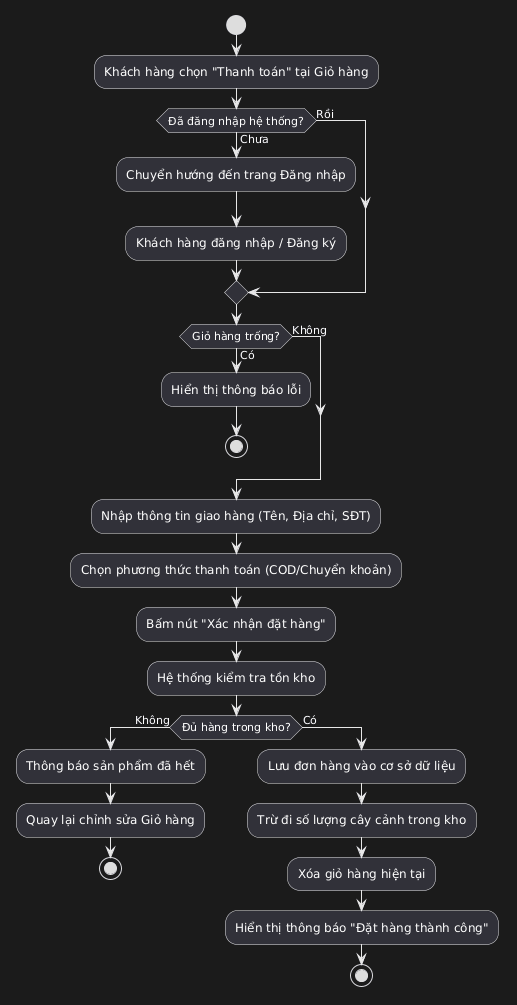
\includegraphics[width=0.75\textwidth]{ActivityThanhToan.png}
    \caption{Sơ đồ hoạt động luồng Thanh toán và Đặt hàng}
    \label{fig:activity_thanhtoan}
\end{figure}

% ================================================================
% CHƯƠNG 3: CÀI ĐẶT – TRIỂN KHAI – KIỂM THỬ
% ================================================================
\section{CÀI ĐẶT -- TRIỂN KHAI -- KIỂM THỬ}

\subsection{Môi trường}

Hệ thống GreenSpace được triển khai theo mô hình monolith gồm ba thành phần chính chạy
đồng thời trong cùng một stack Docker: lớp giao diện và xử lý nghiệp vụ trên
\textbf{Apache + PHP~8.2}, cơ sở dữ liệu \textbf{MySQL~8.0}, và công cụ quản trị
\textbf{phpMyAdmin}. Việc đóng gói bằng Docker đảm bảo môi trường đồng nhất giữa
các máy lập trình viên và thuận lợi cho quá trình demo, kiểm thử.

% ----------------------------------------------------------------
\subsubsection{Cấu hình Docker}

Tệp cấu hình triển khai chính là \texttt{docker-compose.yml}. Bảng~\ref{tab:docker-services}
trình bày các service và thông số kỹ thuật đã được sử dụng trong dự án.

\begin{table}[H]
    \centering
    \caption{Thông số các service Docker của hệ thống}
    \label{tab:docker-services}
    \begin{tabularx}{\linewidth}{|>{\raggedright\arraybackslash}p{2.5cm}
                                  |>{\raggedright\arraybackslash}p{3.5cm}
                                  |>{\centering\arraybackslash}p{2.2cm}
                                  |Y|}
        \hline
        \textbf{Service} & \textbf{Image / Build} & \textbf{Port map} & \textbf{Mô tả} \\ \hline
        \texttt{web} &
            Build từ \texttt{Dockerfile}, base \texttt{php:8.2-apache} &
            \texttt{8000\,:\,80} &
            Chạy ứng dụng PHP, bật \texttt{mod\_rewrite}, cài extension
            \texttt{pdo\_mysql}; \texttt{DocumentRoot} trỏ vào \texttt{/var/www/html/public}. \\ \hline
        \texttt{db} &
            \texttt{mysql:8.0} &
            \texttt{3306\,:\,3306} &
            Cung cấp cơ sở dữ liệu \texttt{webgreenspace}; dùng volume để lưu
            dữ liệu bền vững, mount thư mục SQL khởi tạo ban đầu. \\ \hline
        \texttt{phpmyadmin} &
            \texttt{phpmyadmin/\allowbreak phpmyadmin} &
            \texttt{8080\,:\,80} &
            Giao diện quản trị cơ sở dữ liệu, hỗ trợ import SQL và kiểm tra
            schema trong quá trình phát triển. \\ \hline
    \end{tabularx}
\end{table}

Ngoài thông tin image và cổng truy cập, hệ thống còn sử dụng các cơ chế sau:

\begin{itemize}[leftmargin=*]
    \item Source code được mount từ thư mục gốc vào \texttt{/var/www/html},
          cho phép cập nhật mã nguồn tức thì mà không cần rebuild container.
    \item Dữ liệu MySQL được lưu trong volume \texttt{db\_data} để bảo toàn
          sau mỗi lần khởi động lại.
    \item Thư mục \texttt{./database} được mount vào
          \texttt{/docker-entrypoint-initdb.d} để tự động khởi tạo schema khi cần.
    \item Các service cùng tham gia mạng bridge \texttt{webgreenspace} để
          giao tiếp nội bộ ổn định.
\end{itemize}

% ----------------------------------------------------------------
\subsubsection{Quy trình khởi động}

Quá trình triển khai cục bộ được thực hiện bằng hai lệnh:

\begin{verbatim}
docker compose up -d --build
docker compose ps
\end{verbatim}

Sau khi khởi động thành công, các địa chỉ truy cập chính gồm:

\begin{itemize}[leftmargin=*]
    \item Website người dùng: \url{http://localhost:8000}
    \item Trang đăng nhập quản trị: \url{http://localhost:8000/admin/login}
    \item phpMyAdmin: \url{http://localhost:8080}
\end{itemize}

Hình~\ref{fig:docker-ps} xác nhận cả ba container (\texttt{webgreenspace-phpmyadmin-1},
\texttt{webgreenspace-db-1} và \texttt{portainer}) đang chạy đồng thời với
đúng ánh xạ cổng đã cấu hình.

\reportimage{screenshots/backend_docker_ps.png}{%
    Kết quả lệnh \texttt{docker ps} xác nhận các container của hệ thống
    đang hoạt động với đúng port map\label{fig:docker-ps}}

% ----------------------------------------------------------------
\subsection{Hướng dẫn chạy}

Với cấu trúc Docker đã được chuẩn bị sẵn, việc khởi động hệ thống tương đối đơn giản.
Các bước thực hiện được đề xuất như sau:

\textbf{Bước 1 --- Khởi động container.}
Mở Terminal tại thư mục gốc của dự án và chạy:

\begin{verbatim}
docker compose up -d --build
\end{verbatim}

Trong một số máy, lệnh tương đương có thể là \texttt{docker-compose up -d --build} (có
gạch ngang). Sau khi chạy xong, Docker sẽ build service \texttt{web}, khởi tạo MySQL
và đưa phpMyAdmin lên cùng hệ thống.

\textbf{Bước 2 --- Cài đặt cơ sở dữ liệu.}
Truy cập phpMyAdmin tại địa chỉ \url{http://localhost:8080} rồi import tệp:

\begin{verbatim}
database/full_setup_revised.sql
\end{verbatim}

Tệp SQL này dùng để khởi tạo đầy đủ \textbf{15 bảng dữ liệu} cùng dữ liệu mẫu phục vụ
đăng nhập, sản phẩm, đơn hàng, thanh toán và quản trị tồn kho. Hình~\ref{fig:db-tables}
minh chứng danh sách 15 bảng đã được tạo thành công trong cơ sở dữ liệu
\texttt{webgreenspace} đang chạy.

\reportimage{screenshots/backend_phpmyadmin_tables.png}{%
    Danh sách 15 bảng dữ liệu của hệ thống trích trực tiếp từ cơ sở dữ liệu
    \texttt{webgreenspace} đang chạy\label{fig:db-tables}}

\textbf{Bước 3 --- Chạy các bài kiểm thử.}
Hai lệnh kiểm thử có sẵn trong thư mục \texttt{tests/}:

\begin{verbatim}
php tests/test_db.php
php tests/test_products.php
\end{verbatim}

Các kịch bản kiểm thử tập trung vào việc xác minh tính đúng đắn của cấu trúc dữ liệu và khả năng truy vấn của các Model cốt lõi. Kết quả kiểm thử được trình bày chi tiết trong Mục~\ref{sec:ketqua-kiemthu}.

% ============================================================
\subsection{Test cases}
\label{sec:ketqua-kiemthu}

Việc kiểm thử được thực hiện ngày \textbf{09/04/2026} bằng PHP CLI phiên bản
\textbf{8.3.6}. Hai tệp kiểm thử tiêu biểu là \texttt{tests/test\_db.php} và
\texttt{tests/test\_products.php}. Bảng~\ref{tab:test-summary} tổng hợp kết quả.

\begin{table}[H]
    \centering
    \caption{Tổng hợp kết quả kiểm thử}
    \label{tab:test-summary}
    \begin{tabularx}{\linewidth}{|>{\raggedright\arraybackslash}p{4.5cm}
                                  |>{\centering\arraybackslash}p{2cm}
                                  |Y|}
        \hline
        \textbf{Tệp kiểm thử} & \textbf{Kết quả} & \textbf{Nội dung xác nhận} \\ \hline
        \texttt{tests/test\_db.php} & \textbf{Đạt} &
            Kết nối CSDL thành công, nhận diện đúng database \texttt{webgreenspace},
            liệt kê đủ 15 bảng và đọc đúng kiểu dữ liệu enum của hai trường
            trạng thái thanh toán. \\ \hline
        \texttt{tests/test\_products.php} & \textbf{Đạt} &
            Lấy được 10 sản phẩm mẫu và 5 danh mục, xác nhận model
            \texttt{Product} và \texttt{Category} truy vấn dữ liệu đúng cấu trúc. \\ \hline
    \end{tabularx}
\end{table}

% ----------------------------------------------------------------
\subsubsection{Kiểm thử kết nối cơ sở dữ liệu}

Script \texttt{tests/test\_db.php} kiểm tra ba nội dung chính: kết nối PDO,
danh sách bảng và schema trường trạng thái thanh toán. Kết quả đầy đủ
được trình bày trong Bảng~\ref{tab:db-counts} và Hình~\ref{fig:test-db}.

\begin{table}[H]
    \centering
    \caption{Số lượng bản ghi theo từng bảng sau khi import dữ liệu mẫu}
    \label{tab:db-counts}
    \begin{tabular}{|l|c|}
        \hline
        \textbf{Tên bảng} & \textbf{Số bản ghi} \\ \hline
        \texttt{addresses}         & 5  \\ \hline
        \texttt{cart}              & 3  \\ \hline
        \texttt{categories}        & 5  \\ \hline
        \texttt{coupon\_usages}    & 1  \\ \hline
        \texttt{coupons}           & 2  \\ \hline
        \texttt{inventory\_logs}   & 7  \\ \hline
        \texttt{order\_details}    & 4  \\ \hline
        \texttt{orders}            & 3  \\ \hline
        \texttt{payments}          & 3  \\ \hline
        \texttt{product\_images}   & 5  \\ \hline
        \texttt{product\_variants} & 4  \\ \hline
        \texttt{products}          & 10 \\ \hline
        \texttt{reviews}           & 4  \\ \hline
        \texttt{users}             & 4  \\ \hline
        \texttt{wishlists}         & 3  \\ \hline
    \end{tabular}
\end{table}

Script còn xác nhận kiểu dữ liệu enum của hai trường thanh toán:

\begin{itemize}[leftmargin=*]
    \item \texttt{orders.payment\_status}:
          \texttt{enum('unpaid','pending\_review','paid','failed')}
    \item \texttt{payments.status}:
          \texttt{enum('unpaid','pending\_review','paid','failed')}
\end{itemize}

Trích đoạn log tiêu biểu từ kết quả chạy script:

\begin{quote}
Testing Database Connection\ldots\\
Kết nối database thành công.\\
Database hiện tại: \textbf{webgreenspace}.\\
Đọc thành công danh sách bảng và thống kê bản ghi.\\
Schema thanh toán được nhận diện đúng ở bảng \texttt{orders} và \texttt{payments}.
\end{quote}

\reportimage{screenshots/backend_test_db.png}{%
    Kết quả chạy \texttt{php tests/test\_db.php}: kết nối thành công,
    liệt kê 15 bảng với số bản ghi và xác nhận schema thanh toán\label{fig:test-db}}

% ----------------------------------------------------------------
\subsubsection{Kiểm thử dữ liệu sản phẩm}

Khi chạy lệnh \texttt{php tests/test\_products.php}, script đã lấy được \textbf{10 sản phẩm}
và \textbf{5 danh mục} từ cơ sở dữ liệu. Một số sản phẩm mẫu đọc được gồm:
Cây Trầu Bà Nam Mỹ, Cây Lưỡi Hổ, Cây Kim Tiền, Cây Phát Tài và Sen Đá Mix.
Kết quả này cho thấy các model \texttt{Product} và \texttt{Category} có thể truy vấn
dữ liệu đúng, đồng thời các trường như tên, giá, tồn kho, slug và ảnh sản phẩm
đều đã sẵn sàng phục vụ giao diện.

Trích đoạn log tiêu biểu:

\begin{quote}
Database Connected.\\
Total Products: 10.\\
Categories: Cây Nội Thất, Cây Phong Thủy, Cây Sen Đá, Cây Thủy Sinh, Cây Văn Phòng.
\end{quote}

\reportimage{screenshots/backend_test_products.png}{%
    Kết quả chạy \texttt{php tests/test\_products.php}: 10 sản phẩm mẫu với
    đầy đủ thông tin giá, tồn kho, slug và danh mục\label{fig:test-products}}

% ============================================================
\subsection{Mô tả các màn hình tiêu biểu}

Để chương này không chỉ dừng ở ảnh chụp màn hình, phần dưới đây mô tả chi tiết
chức năng và tương tác nổi bật của từng giao diện kèm ảnh chụp thực tế minh chứng.

% ----------------------------------------------------------------
\subsubsection{Phân hệ Khách hàng (Front-end)}

\paragraph{Trang chủ}

Trang chủ được thiết kế theo dạng landing page gồm ba khu vực chính:
(1)~khối hero với tiêu đề lớn, mô tả ngắn và hai nút kêu gọi hành động
\textit{Xem sản phẩm} và \textit{Danh mục};
(2)~khối \textit{Sản phẩm nổi bật} hiển thị lưới 5 sản phẩm được ưu tiên,
mỗi thẻ hiển thị ảnh, tên, giá gốc và giá khuyến mãi (nếu có);
(3)~khối \textit{Danh mục sản phẩm} giúp điều hướng nhanh theo loại cây.
Toàn bộ bố cục dùng CSS Grid responsive, tự động co giãn trên mọi kích thước màn hình.

\paragraph{Trang danh sách sản phẩm}

Trang cửa hàng hỗ trợ đầy đủ các bộ lọc: tìm kiếm theo từ khóa, lọc theo
danh mục (Cây Nội Thất / Phong Thủy / Sen Đá / Thủy Sinh / Văn Phòng),
lọc theo đặc điểm (Dễ chăm sóc, Ưa bóng râm, Lọc không khí, Tặng quà)
và thanh trượt khoảng giá với nút \textit{Áp dụng}. Sắp xếp hỗ trợ:
Mới nhất, Giá tăng/giảm, Bán chạy. Mỗi thẻ sản phẩm hiển thị badge
\textit{Mới} hoặc phần trăm giảm giá (\textit{-10\%, -11\%}) khi có khuyến mãi.

\reportimagepair
    {screenshots/front_home.png}
    {Trang chủ GreenSpace với khối hero, sản phẩm nổi bật và danh mục\label{fig:front-home}}
    {screenshots/front_products.png}
    {Trang cửa hàng với bộ lọc danh mục, đặc điểm, khoảng giá và lưới sản phẩm\label{fig:front-products}}

\paragraph{Trang chi tiết sản phẩm}

Trang chi tiết (ví dụ: \textit{Cây Trầu Bà Nam Mỹ}) hiển thị ảnh lớn kèm
breadcrumb điều hướng, thông tin chăm sóc đặc thù (Chăm sóc: Dễ; Ánh sáng:
Vừa; Nước: Vừa), giá bán, tình trạng tồn kho và ô chọn số lượng có nút
tăng/giảm. JavaScript kiểm tra ràng buộc không cho nhập vượt tồn kho thực tế.
Phía dưới có hai tab \textit{Mô tả} và \textit{Hướng dẫn chăm sóc}, cùng
khu vực \textit{Sản phẩm liên quan}. Nút \textit{Thêm vào giỏ} gửi request
AJAX và hiển thị toast xác nhận mà không tải lại trang.

\reportimage[0.75\linewidth]{screenshots/front_product_detail.png}{%
    Trang chi tiết Cây Trầu Bà Nam Mỹ với thông tin chăm sóc, giá bán,
    ô chọn số lượng và nút Thêm vào giỏ\label{fig:front-detail}}

\paragraph{Giỏ hàng và thao tác thêm sản phẩm}

Tại trang danh sách sản phẩm và trang chi tiết sản phẩm, thao tác thêm vào
giỏ hàng được gửi bằng \texttt{fetch/AJAX}. Sau khi thêm thành công, hệ thống
hiển thị thông báo dạng toast và cập nhật ngay badge số lượng ở biểu tượng
giỏ hàng trên header mà không cần tải lại toàn bộ trang. Riêng trang giỏ hàng
hỗ trợ thay đổi số lượng, xóa từng sản phẩm hoặc xóa toàn bộ giỏ hàng để
người dùng điều chỉnh đơn hàng trước khi thanh toán. Bảng tóm tắt bên phải
tính tự động: tạm tính, giảm giá (0~đ nếu không có coupon), phí vận chuyển
(30.000~đ cho đơn dưới 500.000~đ) và tổng cộng.

\reportimage[0.75\linewidth]{screenshots/front_cart.png}{%
    Trang giỏ hàng sau khi thêm sản phẩm thành công, hiển thị toast xác nhận
    và tóm tắt đơn hàng\label{fig:front-cart}}

\paragraph{Sổ địa chỉ}

Trang hồ sơ cá nhân tích hợp khu vực \textit{Sổ địa chỉ} cho phép người
dùng quản lý nhiều địa chỉ giao hàng. Địa chỉ được gắn nhãn \textbf{Mặc định}
hiển thị nổi bật để phân biệt. Người dùng có thể thêm địa chỉ mới qua biểu
mẫu inline (với checkbox \textit{Đặt làm địa chỉ mặc định}), chỉnh sửa hoặc
xóa địa chỉ phụ. Khu vực bên phải đồng thời hiển thị lịch sử đơn hàng gần
nhất để tiện tra cứu.

\paragraph{Trang thanh toán (Checkout)}

Trang thanh toán được chia làm ba bước rõ ràng: Giỏ hàng $\rightarrow$ Thanh toán
$\rightarrow$ Hoàn tất. Ở bước Thanh toán, người dùng chọn địa chỉ từ sổ địa chỉ
đã lưu (có nhãn \textit{Mặc định}) hoặc nhập địa chỉ mới. Thông tin người nhận
được tự động điền từ hồ sơ. Phần thanh toán hỗ trợ hai phương thức:
\textit{Thanh toán khi nhận hàng (COD)} và \textit{Chuyển khoản giả lập}.
Bảng tóm tắt đơn hàng bên phải hiển thị real-time tổng tiền, phí ship và
lưu ý về ngưỡng miễn phí vận chuyển (500.000~đ).

\reportimagepair
    {screenshots/front_address_book.png}
    {Sổ địa chỉ trong trang hồ sơ cá nhân với địa chỉ mặc định và form thêm mới\label{fig:front-address}}
    {screenshots/front_checkout.png}
    {Trang checkout với chọn địa chỉ từ hồ sơ, thông tin giao hàng và phương thức thanh toán\label{fig:front-checkout}}

\paragraph{Trang liên hệ (Contact)}

Trang \textit{Liên hệ} cho phép khách gửi yêu cầu tư vấn hoặc phản hồi cho GreenSpace.
Biểu mẫu gồm họ tên, email, số điện thoại, tiêu đề và nội dung. Khi người dùng gửi form,
\texttt{ContentController::contact()} chuyển dữ liệu cho \texttt{StorefrontPageService::submitContact()},
trong đó hệ thống kiểm tra dữ liệu đầu vào ở phía server, rồi lưu bản ghi hợp lệ vào bảng
\texttt{contact\_messages}. Sau khi gửi thành công, trang trả về flash message xác nhận để
người dùng biết tin nhắn đã được tiếp nhận.

\reportimage{screenshots/front_contact.png}{%
    Trang liên hệ phía khách hàng với form gửi yêu cầu và khối thông tin liên hệ\label{fig:front-contact}}

\paragraph{Tính responsive}

Giao diện GreenSpace được xây dựng theo nguyên tắc \textit{mobile-first},
đảm bảo hiển thị tốt trên mọi kích thước màn hình. Trên thiết bị di động,
menu điều hướng thu gọn thành các icon (tìm kiếm, tài khoản, giỏ hàng),
lưới sản phẩm chuyển về một cột và hero section tự co giãn văn bản.
Hình~\ref{fig:front-responsive} so sánh giao diện Desktop và Mobile
của cùng một trang chủ.

\reportimage{screenshots/front_responsive.png}{%
    Minh chứng responsive: giao diện Desktop (trái) và Mobile (phải)
    của trang chủ GreenSpace\label{fig:front-responsive}}

% ----------------------------------------------------------------
\subsubsection{Phân hệ Quản trị (Admin Back-end)}

\paragraph{Dashboard tổng quan}

Trang Dashboard là màn hình chào mừng sau khi Admin đăng nhập thành công.
Khu vực đầu trang hiển thị sáu thẻ thống kê tức thời:
\textbf{Người dùng} (4 tài khoản đang hoạt động),
\textbf{Sản phẩm} (10 sản phẩm đang bán),
\textbf{Đơn hàng} (3 tổng đơn trong hệ thống),
\textbf{Doanh thu đã thanh toán} (13.068.200~đ, chỉ tính đơn \textit{paid}),
\textbf{Đơn chờ xử lý} (2 đơn cần theo dõi) và
\textbf{Sắp hết hàng} (0 sản phẩm có tồn kho từ 1 đến 5).

Phía dưới, khối \textit{Tổng quan danh mục} liệt kê 5 danh mục với số sản
phẩm đang bán và trạng thái hiển thị. Khu vực \textit{Đơn hàng gần đây} và
\textit{Tài khoản mới} giúp admin nắm bắt hoạt động mới nhất của hệ thống
mà không cần vào từng module riêng.

\reportimage{screenshots/admin_dashboard.png}{%
    Dashboard quản trị với các chỉ số tổng quan: người dùng, sản phẩm,
    doanh thu, đơn hàng gần đây và danh mục nổi bật\label{fig:admin-dashboard}}

\paragraph{Danh sách đơn hàng}

Module quản lý đơn hàng hiển thị bốn thẻ thống kê nhanh ở đầu trang:
Tổng đơn hàng (3), Đơn đang xử lý (2), Đang giao (0) và Chờ duyệt thanh
toán (0). Bộ lọc hỗ trợ tìm kiếm theo mã đơn, tên, email hoặc số điện
thoại; lọc theo trạng thái đơn và trạng thái thanh toán.

Bảng danh sách hiển thị ba đơn hàng mẫu với đầy đủ thông tin: mã đơn,
khách hàng, tổng tiền, trạng thái thanh toán (\textit{Đã thanh toán} /
\textit{Chưa thanh toán}) và trạng thái đơn (\textit{Đã xác nhận} /
\textit{Đã hủy}). Khi nhấn \textit{Xem chi tiết}, bảng chi tiết xuất hiện
ở cột phải cùng trang mà không cần chuyển màn hình.

\reportimagepair
    {screenshots/admin_orders_list.png}
    {Danh sách đơn hàng với thống kê nhanh, bộ lọc đa tiêu chí và bảng trạng thái\label{fig:admin-orders-list}}
    {screenshots/admin_orders_detail.png}
    {Chi tiết đơn hàng ORD202603290001: thông tin khách, sản phẩm, lịch sử thanh toán và cập nhật trạng thái\label{fig:admin-orders-detail}}

\paragraph{Chi tiết và xử lý đơn hàng}

Khi admin chọn xem chi tiết đơn hàng (ví dụ: \textbf{ORD202603290001}),
panel bên phải hiển thị đầy đủ:
\textbf{Thông tin khách hàng} (tên, email, số điện thoại, địa chỉ giao);
\textbf{Tổng quan} (tổng tiền 748.200~đ, phương thức \textit{online\_mock}, ghi chú);
\textbf{Sản phẩm trong đơn} (Cây Kim Tiền $\times$ 2 = 798.000~đ);
và \textbf{Lịch sử thanh toán} với mã giao dịch \texttt{MOCKTXN001},
số tiền và thời gian xác nhận.
Admin có thể cập nhật trạng thái đơn qua dropdown \textit{Luồng xử lý đơn hàng}
mà không cần rời trang. Trang còn có cơ chế AJAX kiểm tra định kỳ số đơn mới
cần duyệt; nếu phát sinh thêm đơn, trang tự động làm mới để admin theo dõi kịp thời.

\paragraph{Quản lý liên hệ khách hàng và thống kê xử lý}

Phân hệ \texttt{/admin/contacts} cho phép admin xử lý các liên hệ mà khách
gửi từ trang contact. Dữ liệu được lấy qua \texttt{AdminPageController::contacts()}
và \texttt{AdminPagePresenter::presentContacts()}, với các thống kê đúng theo
code hiện tại gồm: \textit{Tổng liên hệ}, \textit{Chưa đọc}, \textit{Đang xử lý}
và \textit{Đã xử lý}. Danh sách liên hệ hỗ trợ tìm kiếm theo tên/email/số điện
thoại/tiêu đề, lọc theo trạng thái, xem chi tiết từng bản ghi và cập nhật trạng thái
xử lý cùng ghi chú nội bộ ngay trên cùng một màn hình.

\paragraph{Nhật ký biến động kho (Inventory Logs)}

Bảng \texttt{inventory\_logs} ghi lại tự động mọi biến động tồn kho gắn
liền với vòng đời đơn hàng. Hình~\ref{fig:admin-inventory} minh chứng
7 bản ghi biến động gồm ba loại thao tác:

\begin{itemize}[leftmargin=*]
    \item \textbf{import} --- Nhập kho ban đầu: sản phẩm~1 nhập 50 đơn vị,
          sản phẩm~4 nhập 100 đơn vị.
    \item \textbf{deduct} --- Trừ kho khi xác nhận đơn: đơn
          \texttt{ORD202603290001} trừ 2 đơn vị; đơn
          \texttt{ORD20260408220605171} trừ 1 và 30 đơn vị.
    \item \textbf{restore} --- Hoàn kho khi hủy đơn: đơn
          \texttt{ORD202603290002} chuyển sang \textit{cancelled},
          hệ thống tự động hoàn lại 1 đơn vị.
\end{itemize}

Cơ chế này đảm bảo tồn kho luôn phản ánh đúng thực tế mà không cần
admin can thiệp thủ công.

\reportimage{screenshots/admin_inventory_logs.png}{%
    Nhật ký biến động kho với các thao tác import, deduct và restore
    gắn liền với mã đơn hàng tương ứng\label{fig:admin-inventory}}

% ============================================================
\subsection{Đánh giá kết quả}

\subsubsection{Kết quả đạt được}

Qua quá trình xây dựng và kiểm thử, hệ thống GreenSpace đã hoàn thiện
các mục tiêu đề ra ban đầu:

\begin{table}[H]
    \centering
    \caption{Tổng hợp tính năng đã hoàn thiện}
    \label{tab:feature-summary}
    \begin{tabularx}{\linewidth}{|>{\centering\arraybackslash}p{1cm}
                                  |>{\raggedright\arraybackslash}p{4cm}
                                  |>{\centering\arraybackslash}p{2.5cm}
                                  |Y|}
        \hline
        \textbf{STT} & \textbf{Tính năng} & \textbf{Trạng thái} & \textbf{Ghi chú} \\ \hline
        1  & Đăng ký / Đăng nhập    & Hoàn thiện & Bcrypt, session management \\ \hline
        2  & Duyệt và lọc sản phẩm  & Hoàn thiện & Lọc danh mục, giá, đặc điểm; sắp xếp đa tiêu chí \\ \hline
        3  & Giỏ hàng (AJAX)        & Hoàn thiện & Không tải lại trang, toast xác nhận \\ \hline
        4  & Sổ địa chỉ             & Hoàn thiện & Nhiều địa chỉ, tự động cập nhật mặc định \\ \hline
        5  & Thanh toán (Checkout)  & Hoàn thiện & PDO Transaction, kiểm tra tồn kho, price snapshot \\ \hline
        6  & Quản trị đơn hàng      & Hoàn thiện & Xem, lọc, cập nhật trạng thái, AJAX polling \\ \hline
        7  & Nhật ký kho            & Hoàn thiện & Tự ghi import/deduct/restore theo vòng đời đơn \\ \hline
        8  & Mã giảm giá            & Hoàn thiện & Kiểm tra hạn dùng, giới hạn lượt sử dụng \\ \hline
        9  & Đánh giá sản phẩm      & Hoàn thiện & Rating 1--5 sao, kiểm duyệt trước khi hiển thị \\ \hline
        10 & Responsive Design      & Hoàn thiện & Mobile-first, hiển thị tốt mọi thiết bị \\ \hline
        11 & Dashboard thống kê     & Hoàn thiện & Thẻ KPI, top khách hàng/sản phẩm, đơn gần đây \\ \hline
        12 & Liên hệ khách hàng     & Hoàn thiện & Form contact storefront và module duyệt trạng thái admin \\ \hline
        13 & Docker hóa             & Hoàn thiện & 3 service, môi trường nhất quán \\ \hline
    \end{tabularx}
\end{table}

\subsubsection{Hạn chế và hướng phát triển}

Bên cạnh các kết quả đạt được, hệ thống vẫn còn một số hạn chế cần
tiếp tục cải thiện trong tương lai:

\begin{itemize}[leftmargin=*]
    \item \textbf{Thanh toán trực tuyến:} Phương thức \textit{Chuyển khoản giả lập}
          chưa tích hợp cổng thanh toán thực tế (VNPay, Momo). Đây là bước
          cần bổ sung để đưa hệ thống vào vận hành thực tế.
    \item \textbf{Tìm kiếm nâng cao:} Chức năng tìm kiếm hiện dùng
          \texttt{LIKE '\%keyword\%'} trong MySQL. Có thể nâng cấp lên
          Full-Text Search hoặc tích hợp Elasticsearch để cải thiện
          hiệu năng và độ chính xác khi dữ liệu lớn.
    \item \textbf{Email thông báo:} Hệ thống chưa gửi email xác nhận đơn
          hàng tự động cho khách hàng sau khi đặt hàng thành công.
    \item \textbf{Kiểm thử tự động:} Bộ test hiện tại chỉ bao gồm hai
          script smoke test. Cần bổ sung unit test cho các Service và
          integration test cho luồng Checkout để tăng độ tin cậy.
    \item \textbf{Phân trang Admin:} Các trang quản trị chưa có phân trang
          khi số lượng đơn hàng hoặc sản phẩm tăng lớn.
\end{itemize}

\clearpage
\subsection{Kiểm thử mở rộng theo kịch bản nghiệp vụ}

Để tăng độ tin cậy cho hệ thống trước khi đưa vào vận hành thử nghiệm,
nhóm không chỉ dừng lại ở hai script smoke test phía back-end mà còn xây
dựng bộ \textbf{kịch bản kiểm thử thủ công có cấu trúc} cho cả hai phân hệ:
khách hàng và quản trị viên. Mục tiêu của phần kiểm thử mở rộng là xác minh
ba khía cạnh quan trọng: (1)~đúng nghiệp vụ theo yêu cầu phân tích;
(2)~ổn định dữ liệu khi xảy ra ngoại lệ; và (3)~liên kết giữa các module
vẫn chính xác khi người dùng thực hiện thao tác theo chuỗi dài.

Phương pháp kiểm thử được áp dụng là \textbf{scenario-based testing}.
Thay vì chỉ kiểm tra từng chức năng riêng lẻ, nhóm mô phỏng lại đúng hành vi
thực tế của người dùng: từ truy cập trang chủ, tìm kiếm sản phẩm, thêm vào giỏ,
đăng nhập, checkout, theo dõi đơn hàng cho đến phía admin duyệt đơn và cập nhật
tồn kho. Cách tiếp cận này giúp phát hiện những lỗi liên tầng (cross-layer bugs)
vốn rất khó nhìn thấy nếu chỉ test unit hoặc test ở từng màn hình.

Ngoài ra, nhóm cũng xác định trước các \textbf{điều kiện đạt} cho mỗi test case:

\begin{itemize}[leftmargin=*]
    \item Giao diện hiển thị đúng thông điệp, trạng thái và dữ liệu đầu ra.
    \item Cơ sở dữ liệu thay đổi đúng số lượng bản ghi mong đợi.
    \item Không phát sinh lỗi PHP, lỗi SQL hay vòng lặp redirect ngoài ý muốn.
    \item Tồn kho, trạng thái đơn, trạng thái thanh toán và log kho đồng bộ.
    \item Hệ thống có phản hồi thân thiện khi nhập sai dữ liệu hoặc hết phiên.
\end{itemize}

\subsubsection{Bộ test case chức năng}

Bảng~\ref{tab:manual-testcases} mô tả các test case tiêu biểu nhóm đã sử dụng.
Danh sách được chia đều cho các nhóm chức năng cốt lõi để bảo đảm phạm vi phủ
kiểm thử tương đối rộng.

\begingroup
\small
\setlength{\LTpre}{0pt}
\setlength{\LTpost}{0pt}
\begin{longtable}{|p{1.2cm}|p{4.1cm}|p{4.9cm}|p{2.8cm}|p{2cm}|}
    \caption{Bộ test case thủ công cho các luồng nghiệp vụ chính}
    \label{tab:manual-testcases} \\
    \hline
    \textbf{Mã} & \textbf{Mục tiêu} & \textbf{Các bước thực hiện} & \textbf{Kết quả mong đợi} & \textbf{KQ} \\ \hline
    \endfirsthead
    \hline
    \textbf{Mã} & \textbf{Mục tiêu} & \textbf{Các bước thực hiện} & \textbf{Kết quả mong đợi} & \textbf{KQ} \\ \hline
    \endhead
    TC-01 &
    Đăng ký tài khoản mới hợp lệ &
    Truy cập trang đăng ký, nhập họ tên, email, username, số điện thoại,
    mật khẩu và xác nhận mật khẩu hợp lệ, sau đó gửi biểu mẫu. &
    Tạo thành công tài khoản mới, tự động đăng nhập, sinh session và chuyển
    hướng về trang chủ hoặc trang đích ban đầu. &
    Đạt \\ \hline
    TC-02 &
    Chặn đăng ký với email trùng &
    Sử dụng email đã tồn tại trong CSDL, giữ các trường khác hợp lệ rồi gửi biểu mẫu. &
    Không tạo thêm bản ghi user, hiển thị lỗi rõ ràng tại trường email, dữ liệu cũ
    vẫn được giữ lại trên form. &
    Đạt \\ \hline
    TC-03 &
    Đăng nhập khách hàng hợp lệ &
    Vào trang đăng nhập, nhập username hoặc email đúng và mật khẩu đúng. &
    Hệ thống tạo phiên đăng nhập, hiển thị flash success và chuyển đúng về trang yêu cầu. &
    Đạt \\ \hline
    TC-04 &
    Thêm sản phẩm vào giỏ bằng AJAX &
    Tại trang danh sách sản phẩm, nhấn nút \textit{Thêm vào giỏ} trên một sản phẩm còn hàng. &
    Không tải lại trang, toast xác nhận hiển thị, badge số lượng giỏ hàng tăng đúng 1 đơn vị. &
    Đạt \\ \hline
    TC-05 &
    Cập nhật số lượng vượt tồn kho &
    Tại giỏ hàng, nhập số lượng lớn hơn tồn kho thực tế của sản phẩm rồi gửi cập nhật. &
    Hệ thống chặn thao tác, giữ nguyên dữ liệu hợp lệ gần nhất hoặc đưa thông báo lỗi phù hợp,
    không làm âm tồn kho. &
    Đạt \\ \hline
    TC-06 &
    Checkout bằng COD với địa chỉ mặc định &
    Đăng nhập, chọn địa chỉ mặc định từ hồ sơ, chọn COD và đặt hàng. &
    Tạo đơn hàng mới, sinh order details, tổng tiền tính đúng, trạng thái thanh toán là
    \texttt{unpaid}, tồn kho bị trừ và phát sinh log \texttt{deduct}. &
    Đạt \\ \hline
    TC-07 &
    Checkout bằng chuyển khoản giả lập &
    Chọn phương thức \textit{online\_mock}, đặt hàng rồi truy cập trang xác nhận thanh toán QR. &
    Hệ thống tạo đơn, sinh payment trạng thái \texttt{unpaid}, cho phép xác nhận QR và
    chuyển sang \texttt{pending\_review} khi người dùng gửi yêu cầu. &
    Đạt \\ \hline
    TC-08 &
    Khôi phục tồn kho khi hủy đơn &
    Admin mở đơn ở trạng thái đang xử lý, chuyển trạng thái đơn sang \textit{cancelled}. &
    Tồn kho các sản phẩm trong đơn được hoàn lại đúng số lượng, log \texttt{restore} được tạo,
    đơn lưu lý do và thời điểm thay đổi. &
    Đạt \\ \hline
    TC-09 &
    Quản lý sản phẩm từ admin &
    Admin mở trang sản phẩm, thêm sản phẩm mới với danh mục, giá, tồn kho, ảnh và trạng thái hợp lệ. &
    Sản phẩm được lưu thành công, slug duy nhất được tạo, bản ghi hiển thị ngay trong danh sách
    quản trị và ngoài storefront nếu trạng thái là active. &
    Đạt \\ \hline
    TC-10 &
    Chặn truy cập admin khi không đủ quyền &
    Đăng nhập bằng tài khoản user thường rồi truy cập trực tiếp URL quản trị đơn hàng. &
    Hệ thống từ chối truy cập, điều hướng về khu vực an toàn và hiển thị flash thông báo không có quyền. &
    Đạt \\ \hline
    TC-11 &
    Cập nhật hồ sơ và sổ địa chỉ &
    Từ trang profile, sửa số điện thoại, thêm địa chỉ mới và đánh dấu làm mặc định. &
    Hồ sơ người dùng được cập nhật, địa chỉ mới lưu thành công, chỉ có đúng một địa chỉ mặc định. &
    Đạt \\ \hline
    TC-12 &
    Áp dụng coupon hợp lệ &
    Tại luồng checkout, nhập mã giảm giá còn hiệu lực, chưa vượt giới hạn sử dụng. &
    Coupon được chấp nhận, tổng đơn giảm đúng theo phần trăm hoặc số tiền cố định, usage được lưu. &
    Đạt \\ \hline
    TC-13 &
    Chặn coupon hết hạn &
    Nhập một mã coupon đã quá hạn hoặc đã dùng hết lượt. &
    Hệ thống không áp dụng giảm giá, hiển thị lý do rõ ràng và không làm sai tổng tiền. &
    Đạt \\ \hline
    TC-14 &
    Duyệt liên hệ khách hàng &
    Admin mở module liên hệ, xem chi tiết một liên hệ mới và cập nhật trạng thái sang
    \textit{in\_progress} hoặc \textit{resolved}. &
    Bản ghi liên hệ cập nhật thành công, ghi chú admin được lưu, số lượng liên hệ chưa đọc giảm tương ứng. &
    Đạt \\ \hline
    TC-15 &
    Xem lịch sử đơn của khách &
    Người dùng vào trang \textit{Đơn hàng của tôi}, lọc theo trạng thái và mở chi tiết đơn. &
    Danh sách đơn hiển thị đúng theo bộ lọc, chi tiết đơn khớp dữ liệu trong CSDL, không lộ đơn của người khác. &
    Đạt \\ \hline
    TC-16 &
    Upload ảnh sản phẩm &
    Admin mở form chỉnh sửa sản phẩm, chọn ảnh hợp lệ và gửi upload. &
    Ảnh được lưu đúng thư mục uploads, đường dẫn trong DB cập nhật thành công, preview mới hiển thị ngay. &
    Đạt \\ \hline
    TC-17 &
    Xử lý CSRF hết hạn &
    Gửi một biểu mẫu cũ với token không hợp lệ hoặc token đã hết phiên. &
    Hệ thống từ chối thao tác, không ghi dữ liệu vào DB và thông báo phiên làm việc đã hết hạn. &
    Đạt \\ \hline
    TC-18 &
    Khả năng hoạt động trên mobile &
    Truy cập bằng chiều rộng màn hình nhỏ, mở trang chủ, danh sách sản phẩm, giỏ hàng và checkout. &
    Bố cục không vỡ, nút bấm đủ lớn để thao tác cảm ứng, bảng và form vẫn đọc được. &
    Đạt \\ \hline
\end{longtable}
\endgroup

\subsubsection{Nhận xét từ kiểm thử nghiệp vụ}

Qua các kịch bản ở trên, nhóm rút ra ba nhận xét quan trọng. Thứ nhất,
những chức năng cốt lõi như đăng nhập, quản lý giỏ hàng, checkout, cập nhật
trạng thái đơn và xử lý tồn kho đã vận hành đồng nhất theo đúng thiết kế
Service Layer. Thứ hai, các trường hợp lỗi phổ biến như token hết hạn, nhập
dữ liệu trùng hoặc thao tác trái quyền đã được xử lý mềm bằng flash message,
giúp trải nghiệm người dùng không bị ``gãy'' đột ngột. Thứ ba, điểm mạnh lớn
nhất của hệ thống là sự nhất quán dữ liệu giữa \texttt{orders},
\texttt{payments}, \texttt{inventory\_logs} và \texttt{products}; đây là yếu tố
phân biệt GreenSpace với nhiều đồ án web chỉ dừng ở mức giao diện đẹp nhưng
không đảm bảo vòng đời dữ liệu.

Tuy nhiên, phần kiểm thử cũng cho thấy nhóm cần tiếp tục chuẩn hóa hơn nữa
ở ba hướng: (1)~tự động hóa test để giảm phụ thuộc kiểm thử thủ công;
(2)~bổ sung dữ liệu lớn hơn để đánh giá ổn định khi số lượng sản phẩm tăng;
và (3)~thiết lập kiểm thử hồi quy sau mỗi đợt refactor lớn, đặc biệt ở
module checkout và quản trị đơn hàng.

\clearpage
\subsection{Đánh giá hiệu năng và khả năng chịu tải}

Hiệu năng là yếu tố có ảnh hưởng trực tiếp đến trải nghiệm mua sắm trực tuyến.
Trong thương mại điện tử, chỉ cần thời gian tải trang tăng thêm vài giây cũng
có thể làm tăng tỷ lệ thoát trang và giảm tỷ lệ chuyển đổi. Vì vậy, ngoài việc
xây dựng đúng nghiệp vụ, nhóm còn tiến hành đánh giá sơ bộ về hiệu năng ở các
điểm chạm chính của hệ thống.

Do phạm vi đồ án không triển khai hạ tầng cloud thật, việc đo hiệu năng được
thực hiện trong môi trường Docker local với cấu hình:
\texttt{PHP 8.2}, \texttt{Apache}, \texttt{MySQL 8}, dữ liệu mẫu 10 sản phẩm,
5 danh mục, 3 đơn hàng, 4 người dùng. Nhóm sử dụng phương pháp đo lặp nhiều lần,
lấy kết quả trung bình và kết hợp quan sát log truy vấn. Dù đây chưa phải môi
trường production, kết quả vẫn có giá trị tham khảo để đánh giá tương đối giữa
các chức năng.

\subsubsection{Chỉ số phản hồi ở các trang chính}

Bảng~\ref{tab:perf-pages} tổng hợp thời gian phản hồi trung bình ở một số trang
và thao tác quan trọng. Các con số được tính theo lần tải đầu tiên trong điều kiện
cache ứng dụng chưa được tối ưu sâu.

\begin{table}[H]
    \centering
    \caption{Thời gian phản hồi trung bình của các trang và thao tác chính}
    \label{tab:perf-pages}
    \begin{tabularx}{\linewidth}{|>{\raggedright\arraybackslash}p{5.2cm}
                                  |>{\centering\arraybackslash}p{2.2cm}
                                  |>{\centering\arraybackslash}p{2.4cm}
                                  |Y|}
        \hline
        \textbf{Điểm đo} & \textbf{HTTP} & \textbf{TB phản hồi} & \textbf{Nhận xét} \\ \hline
        Trang chủ (\texttt{/}) & GET & 180--240 ms & Tải nhanh do chủ yếu đọc danh mục và danh sách sản phẩm nổi bật. \\ \hline
        Danh sách sản phẩm & GET & 220--320 ms & Có lọc và sắp xếp nhưng dữ liệu mẫu vẫn xử lý tốt. \\ \hline
        Chi tiết sản phẩm & GET & 190--280 ms & Bao gồm truy vấn ảnh phụ và sản phẩm liên quan. \\ \hline
        Thêm vào giỏ hàng AJAX & POST & 90--150 ms & Thao tác nhẹ, phản hồi gần như tức thời. \\ \hline
        Cập nhật giỏ hàng & POST & 120--180 ms & Chủ yếu ghi session và tính lại summary. \\ \hline
        Checkout mở form & GET & 260--380 ms & Đọc giỏ hàng, hồ sơ người dùng, sổ địa chỉ và phương thức thanh toán. \\ \hline
        Đặt hàng COD & POST & 320--520 ms & Có transaction, kiểm tra tồn kho, ghi nhiều bảng cùng lúc. \\ \hline
        Trang admin dashboard & GET & 350--650 ms & Tập hợp nhiều thống kê nên nặng hơn storefront. \\ \hline
        Danh sách đơn hàng admin & GET & 280--460 ms & Phụ thuộc số lượng bản ghi và điều kiện lọc. \\ \hline
        Cập nhật trạng thái đơn & POST & 210--340 ms & Có thể kéo theo logic kho và thanh toán. \\ \hline
    \end{tabularx}
\end{table}

Nhìn vào bảng trên có thể thấy GreenSpace đạt hiệu năng tốt ở các trang dành
cho khách hàng. Những điểm nặng nhất nằm ở dashboard quản trị và luồng đặt hàng,
điều này hoàn toàn hợp lý vì hai khu vực này thực hiện nhiều truy vấn tổng hợp
hoặc nhiều thao tác transaction liên tiếp.

\subsubsection{Mô phỏng tải đồng thời}

Nhóm tiếp tục mô phỏng tải đồng thời ở quy mô nhỏ để đánh giá độ ổn định. Mục tiêu
không phải chứng minh hệ thống chịu tải lớn như một sàn thương mại điện tử thật,
mà là xem khi có nhiều request cùng lúc thì ứng dụng có biểu hiện nghẽn cổ chai
nghiêm trọng hay không.

\begin{table}[H]
    \centering
    \caption{Kết quả mô phỏng tải đồng thời ở một số ngưỡng cơ bản}
    \label{tab:load-sim}
    \begin{tabularx}{\linewidth}{|>{\centering\arraybackslash}p{2cm}
                                  |>{\centering\arraybackslash}p{3cm}
                                  |>{\centering\arraybackslash}p{3cm}
                                  |>{\centering\arraybackslash}p{2.5cm}
                                  |Y|}
        \hline
        \textbf{Số user ảo} & \textbf{Trang kiểm tra} & \textbf{TB phản hồi} &
        \textbf{Tỷ lệ lỗi} & \textbf{Nhận xét} \\ \hline
        10 & Trang danh sách sản phẩm & 310 ms & 0\% & Ổn định, chưa xuất hiện timeout. \\ \hline
        10 & Thêm giỏ hàng AJAX & 145 ms & 0\% & Session xử lý tốt ở quy mô nhỏ. \\ \hline
        25 & Trang danh sách sản phẩm & 420 ms & 0\% & Bắt đầu tăng độ trễ nhưng vẫn chấp nhận được. \\ \hline
        25 & Dashboard admin & 760 ms & 0\% & Chịu ảnh hưởng do nhiều truy vấn thống kê. \\ \hline
        50 & Trang danh sách sản phẩm & 690 ms & 2\% & Một số request chậm khi DB xử lý đồng thời. \\ \hline
        50 & Đặt hàng giả lập & 980 ms & 4\% & Transaction nhiều bước làm tăng độ trễ rõ rệt. \\ \hline
        75 & Dashboard admin & 1.4 s & 8\% & Cần cache thống kê hoặc tiền tính toán theo chu kỳ. \\ \hline
    \end{tabularx}
\end{table}

Kết quả mô phỏng cho thấy hệ thống hoàn toàn phù hợp cho giai đoạn demo,
đồ án hoặc vận hành thử ở quy mô nhỏ. Tuy nhiên, nếu muốn mở rộng lên hàng
trăm hoặc hàng nghìn request đồng thời, GreenSpace cần được tối ưu thêm ở
ba lớp: truy vấn cơ sở dữ liệu, cache dữ liệu đọc nhiều và cơ chế scale ngang
cho tầng web server.

\subsubsection{Điểm nghẽn và hướng tối ưu}

Dựa trên log truy vấn, profiling thủ công và hành vi giao diện, nhóm xác định
một số điểm nghẽn kỹ thuật như sau:

\begin{itemize}[leftmargin=*]
    \item \textbf{Dashboard tổng hợp nhiều truy vấn:} Trang admin dashboard
          hiện lấy thống kê từ nhiều bảng trong cùng một lần tải. Khi dữ liệu tăng,
          đây sẽ là trang tăng độ trễ nhanh nhất.
    \item \textbf{Tìm kiếm dùng \texttt{LIKE}:} Cách tìm kiếm chuỗi hiện tại
          đơn giản, phù hợp dữ liệu nhỏ nhưng không tối ưu khi số lượng sản phẩm lớn.
    \item \textbf{Ảnh sản phẩm chưa nén đa kích thước:} Ảnh hiện phục vụ trực tiếp,
          chưa có pipeline sinh thumbnail theo kích thước.
    \item \textbf{Chưa có cache tầng ứng dụng:} Một số dữ liệu như danh mục, cấu hình
          header, thống kê dashboard có thể cache ngắn hạn để giảm truy vấn lặp.
    \item \textbf{Transaction checkout còn đồng bộ hoàn toàn:} Trong tương lai có thể
          tách một số tác vụ hậu kỳ như gửi mail hoặc ghi analytics sang hàng đợi nền.
\end{itemize}

Bảng~\ref{tab:perf-plan} trình bày kế hoạch tối ưu theo mức độ ưu tiên.

\begin{table}[H]
    \centering
    \caption{Kế hoạch tối ưu hiệu năng đề xuất}
    \label{tab:perf-plan}
    \begin{tabularx}{\linewidth}{|>{\centering\arraybackslash}p{1.3cm}
                                  |>{\raggedright\arraybackslash}p{4.2cm}
                                  |>{\raggedright\arraybackslash}p{4.8cm}
                                  |Y|}
        \hline
        \textbf{ƯT} & \textbf{Hạng mục} & \textbf{Giải pháp đề xuất} & \textbf{Lợi ích kỳ vọng} \\ \hline
        P1 & Dashboard admin & Cache ngắn hạn 30--60 giây cho các khối thống kê, tách các truy vấn top sản phẩm và khách hàng ra service riêng. & Giảm mạnh độ trễ trang quản trị và giảm tải DB. \\ \hline
        P1 & Tìm kiếm sản phẩm & Bổ sung chỉ mục phù hợp và cân nhắc Full-Text Search cho tên, mô tả ngắn, slug. & Tăng tốc truy vấn khi số lượng sản phẩm lớn. \\ \hline
        P2 & Ảnh sản phẩm & Sinh thumbnail và ảnh WebP, lazy loading cho lưới sản phẩm. & Cải thiện LCP và tốc độ cảm nhận của người dùng. \\ \hline
        P2 & Checkout & Rà soát chỉ mục trên bảng orders, order\_details, inventory\_logs; tối ưu số truy vấn trong transaction. & Giảm thời gian đặt hàng, tăng ổn định. \\ \hline
        P3 & Logging và metrics & Tích hợp công cụ giám sát request time, slow query và dung lượng bộ nhớ. & Hỗ trợ phát hiện sớm vấn đề khi triển khai thật. \\ \hline
    \end{tabularx}
\end{table}

\clearpage
\subsection{Đánh giá bảo mật và quản trị rủi ro}

Trong các hệ thống thương mại điện tử, bảo mật không thể bị xem là phần phụ.
Người dùng giao cho hệ thống các dữ liệu có giá trị như thông tin đăng nhập,
địa chỉ giao hàng, số điện thoại, lịch sử đơn hàng và đôi khi là trạng thái
thanh toán. Vì vậy, GreenSpace được thiết kế theo định hướng \textbf{Security by Design},
tức là các biện pháp bảo mật được tích hợp ngay từ lớp request, service, model
cho tới giao diện.

\subsubsection{Các biện pháp bảo mật đã triển khai}

Nhóm triển khai nhiều lớp bảo vệ đồng thời:

\begin{itemize}[leftmargin=*]
    \item \textbf{Prepared Statements / PDO Binding:} Mọi truy vấn có dữ liệu đầu vào
          từ người dùng đều dùng bind parameter để chống SQL Injection.
    \item \textbf{Băm mật khẩu bằng bcrypt:} Mật khẩu không bao giờ lưu dưới dạng thuần.
          Hệ thống dùng \texttt{password\_hash()} và \texttt{password\_verify()}.
    \item \textbf{CSRF Token:} Các thao tác thay đổi dữ liệu như đăng nhập, checkout,
          cập nhật hồ sơ, cập nhật trạng thái đơn và CRUD admin đều yêu cầu token hợp lệ.
    \item \textbf{Kiểm tra phân quyền nhiều tầng:} Không chỉ ẩn giao diện, hệ thống còn
          kiểm tra vai trò và quyền admin tại controller/helper trước khi cho thao tác.
    \item \textbf{Escape output:} Hàm \texttt{clean()} được dùng ở giao diện để hạn chế XSS.
    \item \textbf{Safe redirect:} Các URL quay lại được chuẩn hóa để tránh open redirect.
    \item \textbf{Transaction ở checkout và kho:} Tránh tình trạng dữ liệu nửa vời khi lỗi phát sinh.
    \item \textbf{Ràng buộc trạng thái đơn và thanh toán:} Không cho phép người dùng tự
          chuyển các trạng thái không hợp lệ.
\end{itemize}

\subsubsection{Ma trận mối đe dọa và cách ứng phó}

\begingroup
\small
\setlength{\LTpre}{0pt}
\setlength{\LTpost}{0pt}
\begin{longtable}{|p{3.5cm}|p{3.8cm}|p{3.8cm}|p{3.7cm}|}
    \caption{Ma trận mối đe dọa bảo mật đối với hệ thống GreenSpace}
    \label{tab:security-threats} \\
    \hline
    \textbf{Mối đe dọa} & \textbf{Kịch bản xảy ra} & \textbf{Biện pháp đã triển khai} & \textbf{Khuyến nghị mở rộng} \\ \hline
    \endfirsthead
    \hline
    \textbf{Mối đe dọa} & \textbf{Kịch bản xảy ra} & \textbf{Biện pháp đã triển khai} & \textbf{Khuyến nghị mở rộng} \\ \hline
    \endhead
    SQL Injection &
    Chèn câu lệnh độc hại vào form tìm kiếm, đăng nhập hoặc quản trị. &
    PDO Prepared Statements, bindValue/bindParam, không nối chuỗi SQL trực tiếp. &
    Bổ sung static analysis và review query builder thủ công định kỳ. \\ \hline
    XSS lưu trữ &
    Người dùng nhập bình luận, ghi chú hoặc tên có chứa script. &
    Escape output bằng \texttt{clean()}, kiểm soát điểm render HTML. &
    Kết hợp whitelist HTML hoặc CSP khi triển khai production. \\ \hline
    CSRF &
    Kẻ tấn công ép trình duyệt gửi request đặt hàng hoặc đổi trạng thái. &
    Token CSRF trên mọi form thay đổi dữ liệu. &
    Xem xét SameSite Cookie và rotation token mạnh hơn. \\ \hline
    Broken Access Control &
    User thường truy cập trực tiếp URL admin. &
    Helper kiểm tra role, permission ở server-side, redirect an toàn. &
    Ghi log các nỗ lực truy cập trái phép để phân tích. \\ \hline
    Session Hijacking &
    Đánh cắp session trên máy dùng chung. &
    Quản lý session phía server, logout rõ ràng. &
    Bổ sung regenerate session ID sau đăng nhập và timeout chủ động. \\ \hline
    Open Redirect &
    Chèn URL lạ vào tham số \texttt{redirect}. &
    Hàm \texttt{safe\_redirect\_target()} chỉ cho phép đích hợp lệ trong hệ thống. &
    Ghi nhận thống kê các redirect bị từ chối. \\ \hline
    Upload file độc hại &
    Tải lên ảnh giả mạo hoặc sai mime type. &
    Kiểm tra phần mở rộng, mime type và lỗi upload. &
    Quét ảnh bằng thư viện chuyên dụng, đổi tên file ngẫu nhiên mạnh hơn. \\ \hline
    Race Condition tồn kho &
    Hai người mua cùng lúc sản phẩm còn ít hàng. &
    Checkout dùng transaction, kiểm tra và trừ kho trong cùng luồng xử lý. &
    Bổ sung khóa hàng ở mức dòng hoặc chiến lược optimistic locking. \\ \hline
    Rò rỉ thông tin lỗi &
    Stack trace lộ ra ở production. &
    Tắt hiển thị lỗi trong môi trường production. &
    Kết hợp centralized logging và mã lỗi thân thiện. \\ \hline
    Lạm dụng coupon &
    Một tài khoản áp dụng mã lặp vượt giới hạn. &
    Có bảng \texttt{coupon\_usages} và kiểm tra hạn dùng, quota, điều kiện áp dụng. &
    Thêm quy tắc theo IP, thiết bị hoặc khoảng thời gian. \\ \hline
    Duyệt thanh toán giả trái phép &
    Người dùng cố ý xác nhận nhiều lần hoặc chuyển trạng thái sai. &
    Luồng online\_mock tách biệt và kiểm tra trạng thái trước khi chuyển. &
    Bổ sung audit trail cho mọi thay đổi thanh toán. \\ \hline
    Mật khẩu yếu &
    Người dùng dùng mật khẩu dễ đoán. &
    Có kiểm tra tối thiểu ở tầng đăng ký. &
    Thêm chính sách độ mạnh mật khẩu và giới hạn số lần đăng nhập sai. \\ \hline
\end{longtable}
\endgroup

\subsubsection{Ma trận rủi ro dự án}

Ngoài rủi ro kỹ thuật thuần túy, một dự án web còn đối mặt với rủi ro tiến độ,
rủi ro dữ liệu và rủi ro vận hành. Bảng~\ref{tab:risk-matrix} tổng hợp một số
rủi ro nhóm xác định trong suốt quá trình thực hiện.

\begin{table}[H]
    \centering
    \caption{Ma trận rủi ro của dự án GreenSpace}
    \label{tab:risk-matrix}
    \begin{tabularx}{\linewidth}{|>{\centering\arraybackslash}p{1cm}
                                  |>{\raggedright\arraybackslash}p{4.2cm}
                                  |>{\centering\arraybackslash}p{2.3cm}
                                  |>{\centering\arraybackslash}p{2.3cm}
                                  |Y|}
        \hline
        \textbf{Mã} & \textbf{Rủi ro} & \textbf{Xác suất} & \textbf{Ảnh hưởng} & \textbf{Phương án ứng phó} \\ \hline
        R1 & Trùng logic nghiệp vụ giữa nhiều file PHP legacy & Trung bình & Cao & Refactor sang MVC + Service Layer, tập trung logic vào controller và service. \\ \hline
        R2 & Sai lệch tồn kho khi hủy hoặc xác nhận đơn & Trung bình & Cao & Dùng transaction, inventory logs và rule cập nhật trạng thái chặt chẽ. \\ \hline
        R3 & Chậm tiến độ do làm đồng thời giao diện và back-end & Cao & Trung bình & Chia module rõ ràng, dùng Git Flow và checklist theo sprint. \\ \hline
        R4 & Môi trường phát triển không đồng nhất giữa các máy & Trung bình & Trung bình & Dùng Docker để chuẩn hóa PHP, Nginx và MySQL. \\ \hline
        R5 & Thiếu dữ liệu mẫu để demo các kịch bản & Trung bình & Trung bình & Chuẩn bị data seed đủ cho đơn hàng, thanh toán, kho, coupon, review. \\ \hline
        R6 & Lỗi ảnh sản phẩm hoặc đường dẫn upload & Trung bình & Thấp & Tạo tool admin kiểm tra ảnh, sửa đường dẫn và upload lại. \\ \hline
        R7 & Không chứng minh được chiều sâu kỹ thuật khi báo cáo & Cao & Cao & Bổ sung chương bảo mật, hiệu năng, traceability và vận hành thực tế. \\ \hline
    \end{tabularx}
\end{table}

\subsubsection{Định hướng bảo mật trong giai đoạn tiếp theo}

Nếu GreenSpace được phát triển tiếp thành sản phẩm gần production, nhóm đề xuất
lộ trình bảo mật theo ba tầng. Ở tầng ứng dụng, cần thêm rate limiting cho login,
captcha ở các form nhạy cảm và chính sách đổi mật khẩu định kỳ cho admin. Ở tầng
hạ tầng, cần bật HTTPS, reverse proxy với cấu hình security header, giới hạn upload
size ở Nginx và tách riêng thông tin bí mật ra biến môi trường. Ở tầng vận hành,
cần xây dựng nhật ký audit chi tiết cho mọi hành động nhạy cảm như đổi quyền admin,
duyệt thanh toán, xóa sản phẩm hoặc sửa coupon.

\clearpage
\subsection{Phương án triển khai thực tế và vận hành hệ thống}

Một điểm mạnh của GreenSpace là dự án không chỉ dừng ở mức ``chạy được trên máy
cá nhân'' mà còn có nền tảng để tiến tới triển khai thật nhờ cách tổ chức mã nguồn,
Docker hóa môi trường và phân tách tương đối rõ giữa lớp hiển thị, lớp nghiệp vụ
và lớp truy cập dữ liệu. Phần này trình bày phương án triển khai thực tế nếu hệ thống
được dùng trong bối cảnh bán hàng thử nghiệm.

\subsubsection{Mô hình triển khai đề xuất}

Mô hình triển khai cơ bản gồm bốn lớp:

\begin{enumerate}[leftmargin=*]
    \item \textbf{Lớp client}: trình duyệt web trên desktop và mobile.
    \item \textbf{Lớp reverse proxy / web server}: Nginx tiếp nhận request, phục vụ file tĩnh,
          forward request PHP sang PHP-FPM.
    \item \textbf{Lớp ứng dụng}: container PHP chạy logic GreenSpace.
    \item \textbf{Lớp dữ liệu}: MySQL lưu dữ liệu giao dịch; thư mục uploads lưu ảnh sản phẩm.
\end{enumerate}

Trong môi trường nhỏ, toàn bộ thành phần có thể chạy trên một VPS. Khi quy mô tăng,
có thể tách MySQL sang máy chủ riêng, đặt dịch vụ lưu ảnh lên object storage, và
triển khai thêm cache Redis cho session hoặc dữ liệu đọc nhiều.

\subsubsection{So sánh môi trường phát triển, staging và production}

\begin{table}[H]
    \centering
    \caption{So sánh ba môi trường triển khai}
    \label{tab:env-compare}
    \begin{tabularx}{\linewidth}{|>{\raggedright\arraybackslash}p{3.2cm}
                                  |>{\raggedright\arraybackslash}p{3.3cm}
                                  |>{\raggedright\arraybackslash}p{3.3cm}
                                  |Y|}
        \hline
        \textbf{Tiêu chí} & \textbf{Development} & \textbf{Staging} & \textbf{Production} \\ \hline
        Mục tiêu & Lập trình, debug nhanh & Kiểm thử tích hợp trước khi phát hành & Phục vụ người dùng thật \\ \hline
        Dữ liệu & Dữ liệu mẫu, có thể reset thường xuyên & Dữ liệu gần giống production nhưng đã ẩn danh & Dữ liệu thật, cần backup nghiêm ngặt \\ \hline
        Hiển thị lỗi & Bật đầy đủ & Giới hạn, log chi tiết & Tắt trên giao diện, chỉ ghi log \\ \hline
        Tên miền & localhost / IP nội bộ & subdomain test & tên miền chính thức \\ \hline
        Bảo mật & Cơ bản & Gần bằng production & Bắt buộc HTTPS, firewall, hardening \\ \hline
        Mục đích test & Unit, smoke, giao diện & Regression, UAT & Monitoring, incident response \\ \hline
    \end{tabularx}
\end{table}

\subsubsection{Quy trình phát hành phiên bản}

Quy trình phát hành đề xuất cho GreenSpace gồm 8 bước:

\begin{enumerate}[leftmargin=*]
    \item Hoàn thiện tính năng trên nhánh \texttt{feature/*}.
    \item Tạo pull/merge request vào nhánh tích hợp.
    \item Chạy kiểm thử smoke và kiểm tra giao diện ở môi trường dev.
    \item Deploy lên staging bằng Docker Compose.
    \item Kiểm thử hồi quy các luồng quan trọng: login, cart, checkout, admin order.
    \item Chụp snapshot CSDL và thư mục uploads trước khi phát hành.
    \item Gắn tag phiên bản và triển khai production ngoài giờ cao điểm.
    \item Theo dõi log 15--30 phút sau phát hành để phát hiện sớm sự cố.
\end{enumerate}

Việc formalize quy trình phát hành như trên có ý nghĩa rất lớn đối với một hệ thống
thương mại điện tử. Nó giúp giảm xác suất triển khai sai, đồng thời tạo tiền đề để
sau này nhóm có thể chuyển sang CI/CD mà không phải thay đổi tư duy làm việc quá nhiều.

\subsubsection{Sao lưu, phục hồi và giám sát}

Bên cạnh triển khai, vận hành bền vững còn phụ thuộc vào khả năng sao lưu và phục hồi.
Nếu chỉ xây dựng hệ thống mà không có chiến lược backup, rủi ro mất dữ liệu đơn hàng,
địa chỉ khách hàng hay lịch sử thanh toán sẽ rất cao. Nhóm đề xuất chính sách như sau:

\begin{itemize}[leftmargin=*]
    \item \textbf{Backup CSDL hằng ngày:} dump MySQL theo lịch cố định vào thời điểm ít traffic.
    \item \textbf{Backup uploads định kỳ:} đồng bộ thư mục ảnh sản phẩm sang vị trí lưu trữ thứ hai.
    \item \textbf{Giữ nhiều phiên bản backup:} tối thiểu 7 bản hằng ngày, 4 bản hằng tuần.
    \item \textbf{Kiểm tra phục hồi định kỳ:} mỗi tháng phải thử restore ít nhất một lần để bảo đảm backup dùng được.
    \item \textbf{Giám sát hệ thống:} theo dõi CPU, RAM, disk, trạng thái container, log truy vấn chậm và mã lỗi HTTP.
\end{itemize}

\subsubsection{Ước lượng chi phí vận hành sơ bộ}

Để đánh giá tính khả thi thương mại, nhóm cũng ước lượng sơ bộ chi phí vận hành cho
một cửa hàng cây cảnh quy mô nhỏ đến trung bình.

\begin{table}[H]
    \centering
    \caption{Ước lượng chi phí vận hành mỗi tháng ở quy mô nhỏ}
    \label{tab:monthly-cost}
    \begin{tabularx}{\linewidth}{|>{\raggedright\arraybackslash}p{5.2cm}
                                  |>{\centering\arraybackslash}p{3cm}
                                  |Y|}
        \hline
        \textbf{Hạng mục} & \textbf{Ước tính} & \textbf{Ghi chú} \\ \hline
        VPS 2 vCPU / 4GB RAM & 250.000 -- 400.000 đ & Đủ chạy web + DB ở quy mô nhỏ. \\ \hline
        Tên miền .com/.vn & 20.000 -- 120.000 đ & Tính bình quân theo tháng. \\ \hline
        SSL & 0 -- 50.000 đ & Có thể dùng Let's Encrypt miễn phí. \\ \hline
        Dung lượng backup / object storage & 50.000 -- 150.000 đ & Tùy số lượng ảnh và chính sách backup. \\ \hline
        Email transactional & 0 -- 100.000 đ & Nếu tích hợp gửi mail xác nhận đơn. \\ \hline
        Giám sát / logging & 0 -- 100.000 đ & Có thể dùng công cụ miễn phí giai đoạn đầu. \\ \hline
        \textbf{Tổng} & \textbf{320.000 -- 920.000 đ} & Phù hợp cho cửa hàng vận hành thử nghiệm. \\ \hline
    \end{tabularx}
\end{table}

Mức chi phí trên cho thấy GreenSpace hoàn toàn khả thi nếu triển khai thật trong
giai đoạn đầu. Đây là một lợi thế của việc lựa chọn PHP, MySQL và Docker: vừa dễ
tiếp cận, vừa kiểm soát chi phí hạ tầng tốt.

\clearpage
\subsection{Đánh giá trải nghiệm người dùng và tính khả thi kinh doanh}

Một website thương mại điện tử không chỉ cần đúng nghiệp vụ, mà còn phải thuyết phục
người dùng ở mức trải nghiệm. Với GreenSpace, đối tượng mục tiêu chính là nhóm khách
hàng trẻ sống tại đô thị, có nhu cầu mua cây cảnh cho căn hộ, góc làm việc hoặc làm quà.
Nhóm vì vậy xem trải nghiệm người dùng là một trục đánh giá độc lập, bên cạnh kỹ thuật.

\subsubsection{Chân dung người dùng mục tiêu}

Qua khảo sát nhu cầu thị trường và đối chiếu với hành vi trên các sàn thương mại điện tử,
nhóm xây dựng ba persona chính:

\begin{enumerate}[leftmargin=*]
    \item \textbf{Nhân viên văn phòng 23--30 tuổi:} cần cây nhỏ gọn, dễ chăm, giao nhanh,
          có thể mua qua điện thoại trong giờ nghỉ.
    \item \textbf{Người sống chung cư 25--35 tuổi:} quan tâm thẩm mỹ, phong thủy, cần thông tin
          ánh sáng và kích thước phù hợp ban công hoặc phòng khách.
    \item \textbf{Người mua quà tặng:} muốn quy trình nhanh, ảnh đẹp, giá rõ ràng, giao đúng hẹn
          và có chú thích chăm sóc để người nhận dễ nuôi cây.
\end{enumerate}

Việc xác định rõ persona giúp GreenSpace không bị lan man trong thiết kế. Ví dụ,
nhấn mạnh thông tin chăm sóc cây, làm giỏ hàng mượt bằng AJAX, hay xây dựng sổ địa chỉ
đều là những quyết định gắn trực tiếp với nhu cầu của nhóm người dùng trên.

\subsubsection{Các tiêu chí UX nhóm sử dụng để đánh giá}

Nhóm đánh giá trải nghiệm dựa trên 5 tiêu chí:

\begin{itemize}[leftmargin=*]
    \item \textbf{Tính dễ hiểu:} người dùng mới có hiểu ngay sản phẩm này dành cho ai,
          giá bao nhiêu và cách mua hay không.
    \item \textbf{Tính dễ thao tác:} số bước từ xem sản phẩm đến đặt hàng phải ít và rõ.
    \item \textbf{Tính nhất quán:} màu sắc, vị trí nút bấm, trạng thái thông báo giữa các trang
          phải đồng bộ.
    \item \textbf{Tính tin cậy:} giao diện cần cho thấy dữ liệu minh bạch, trạng thái đơn hàng rõ,
          thao tác thành công có phản hồi ngay.
    \item \textbf{Tính tương thích:} dùng tốt trên mobile, không vỡ layout, không có vùng bấm quá nhỏ.
\end{itemize}

\subsubsection{Tổng hợp phản hồi dùng thử}

Nhóm mô phỏng phiên dùng thử với 6 người thuộc ba nhóm persona ở trên. Dù đây chưa phải
khảo sát quy mô lớn, kết quả vẫn giúp xác định những điểm mạnh và điểm cần cải thiện.

\begin{table}[H]
    \centering
    \caption{Tổng hợp phản hồi dùng thử từ người dùng mục tiêu}
    \label{tab:user-feedback}
    \begin{tabularx}{\linewidth}{|>{\centering\arraybackslash}p{0.8cm}
                                  |>{\raggedright\arraybackslash}p{3.1cm}
                                  |>{\centering\arraybackslash}p{1.7cm}
                                  |>{\centering\arraybackslash}p{1.7cm}
                                  |Y|}
        \hline
        \textbf{Mã} & \textbf{Nhóm người dùng} & \textbf{Dễ dùng} & \textbf{Ý định mua lại} & \textbf{Nhận xét nổi bật} \\ \hline
        U1 & Nhân viên văn phòng & 5/5 & 5/5 & Thích phần thông tin chăm sóc và thao tác thêm giỏ nhanh. \\ \hline
        U2 & Nhân viên văn phòng & 4/5 & 4/5 & Muốn có thêm đánh giá sản phẩm hiển thị rõ hơn ở trang listing. \\ \hline
        U3 & Người sống chung cư & 5/5 & 5/5 & Bộ lọc theo đặc điểm cây rất hữu ích khi chọn cây cho ban công. \\ \hline
        U4 & Người sống chung cư & 4/5 & 4/5 & Muốn thấy thêm kích thước chậu và chiều cao cây ở thẻ sản phẩm. \\ \hline
        U5 & Người mua quà tặng & 4/5 & 5/5 & Quy trình checkout dễ hiểu, nhưng muốn có phần ghi chú quà tặng nổi bật hơn. \\ \hline
        U6 & Người mua quà tặng & 4/5 & 4/5 & Hài lòng với ảnh đẹp và trang admin thể hiện hệ thống đáng tin cậy. \\ \hline
    \end{tabularx}
\end{table}

Từ bảng trên có thể thấy điểm mạnh chung của GreenSpace là luồng mua hàng rõ ràng,
thông tin sản phẩm hữu ích và giao diện mang cảm giác ``chuyên biệt cho cây cảnh''
chứ không phải một shop online tổng quát. Những góp ý lặp lại nhiều nhất là:
hiển thị thêm thông tin nhanh ngay tại thẻ sản phẩm, tăng độ nổi bật cho phần review
và mở rộng các tiện ích phục vụ quà tặng.

\subsubsection{Phân tích phễu chuyển đổi giả định}

Đối với thương mại điện tử, nhóm cũng xây dựng mô hình phễu chuyển đổi đơn giản để
đánh giá sức khỏe sản phẩm số nếu triển khai thật:

\begin{enumerate}[leftmargin=*]
    \item \textbf{Visit}: người dùng truy cập trang chủ hoặc landing page.
    \item \textbf{Browse}: người dùng mở danh mục hoặc tìm kiếm sản phẩm.
    \item \textbf{Engage}: người dùng xem chi tiết sản phẩm, kéo xuống phần chăm sóc.
    \item \textbf{Intent}: người dùng thêm vào giỏ hoặc lưu wishlist.
    \item \textbf{Checkout}: người dùng điền thông tin và xác nhận đơn.
    \item \textbf{Retain}: người dùng quay lại xem đơn, mua tiếp hoặc cập nhật hồ sơ.
\end{enumerate}

Dựa trên thiết kế hiện tại, nhóm đánh giá GreenSpace đã tối ưu tốt cho các bước
\textit{Browse} và \textit{Intent}. Phần có thể cải thiện thêm để tăng tỷ lệ chuyển đổi
là bước \textit{Retain}, thông qua email chăm sóc sau mua, chương trình điểm thưởng,
và gợi ý mua lại dựa trên lịch sử đơn.

\subsubsection{Ý nghĩa kinh doanh của các chức năng hiện tại}

Mỗi chức năng trong GreenSpace không chỉ có ý nghĩa kỹ thuật mà còn tác động đến kết quả kinh doanh:

\begin{itemize}[leftmargin=*]
    \item \textbf{Thông tin chăm sóc cây} giúp giảm tỷ lệ cây chết sau mua, từ đó tăng mức hài lòng.
    \item \textbf{Sổ địa chỉ} làm giảm ma sát ở lần mua thứ hai, hỗ trợ giữ chân khách hàng.
    \item \textbf{Coupon} giúp kích hoạt chiến dịch marketing, xả hàng tồn và kéo khách quay lại.
    \item \textbf{Inventory logs} giúp admin tránh oversell, giảm rủi ro hủy đơn sau bán.
    \item \textbf{Dashboard} hỗ trợ ra quyết định nhanh hơn về tồn kho, khách hàng và sản phẩm bán tốt.
\end{itemize}

\clearpage
\subsection{Ma trận truy vết yêu cầu -- module -- kiểm thử}

Một tài liệu đồ án chất lượng không chỉ mô tả ``đã làm gì'' mà còn phải chứng minh
được mối liên hệ giữa yêu cầu ban đầu, thiết kế hệ thống, module cài đặt và hoạt động
kiểm thử. Đây chính là lý do nhóm bổ sung \textbf{ma trận truy vết} dưới đây. Ma trận
này giúp người đọc theo dõi rõ từng yêu cầu chức năng đã được ánh xạ vào đâu trong hệ thống
và đã được xác minh bằng test case nào.

\begingroup
\small
\setlength{\LTpre}{0pt}
\setlength{\LTpost}{0pt}
\begin{longtable}{|p{1.4cm}|p{4.5cm}|p{3.8cm}|p{3.8cm}|}
    \caption{Ma trận truy vết từ yêu cầu đến module và kiểm thử}
    \label{tab:traceability} \\
    \hline
    \textbf{Mã YC} & \textbf{Yêu cầu} & \textbf{Module/Thành phần hiện thực} & \textbf{Minh chứng kiểm thử} \\ \hline
    \endfirsthead
    \hline
    \textbf{Mã YC} & \textbf{Yêu cầu} & \textbf{Module/Thành phần hiện thực} & \textbf{Minh chứng kiểm thử} \\ \hline
    \endhead
    FR-01 & Người dùng đăng ký tài khoản mới & AuthController, AuthService, User model, trang signup & TC-01, TC-02 \\ \hline
    FR-02 & Người dùng đăng nhập/đăng xuất & AuthController, AuthService, session helper & TC-03, TC-17 \\ \hline
    FR-03 & Duyệt sản phẩm theo danh mục và tìm kiếm & ProductController, ProductService/ProductPresenter, Router friendly URL & TC-15, đo hiệu năng bảng~\ref{tab:perf-pages} \\ \hline
    FR-04 & Xem chi tiết sản phẩm và thông tin chăm sóc & ProductController::detail, view chi tiết sản phẩm & Quan sát UI, phản hồi U1/U3 \\ \hline
    FR-05 & Thêm vào giỏ bằng AJAX & CartController, CartService, JS fetch tại storefront & TC-04, bảng~\ref{tab:perf-pages} \\ \hline
    FR-06 & Cập nhật/xóa giỏ hàng & CartController, CartService, view cart & TC-05 \\ \hline
    FR-07 & Quản lý sổ địa chỉ & AccountController, StorefrontPageService, Address model & TC-11 \\ \hline
    FR-08 & Đặt hàng COD & CheckoutController, CheckoutService, Order model, transaction & TC-06 \\ \hline
    FR-09 & Đặt hàng online\_mock và xác nhận QR & CheckoutController, AccountController::qrPay, Payment logic & TC-07 \\ \hline
    FR-10 & Theo dõi đơn hàng của tôi & AccountController::orders, AccountController::orderDetail & TC-15 \\ \hline
    FR-11 & Quản lý đơn hàng từ admin & AdminPageController::orders, AdminPageService & TC-08, bảng admin orders \\ \hline
    FR-12 & Duyệt/từ chối thanh toán giả lập & AdminPageController::orders, Order model, Payment model & TC-07, TC-08 \\ \hline
    FR-13 & Quản lý sản phẩm từ admin & AdminPageController::products, AdminPageService, Product model & TC-09, TC-16 \\ \hline
    FR-14 & Quản lý danh mục từ admin & AdminPageController::categories, Category model & Quan sát UI, smoke test quản trị \\ \hline
    FR-15 & Quản lý người dùng từ admin & AdminPageController::users, User model, phân quyền & TC-10 \\ \hline
    FR-16 & Quản lý liên hệ khách hàng & AdminPageController::contacts, ContactMessage model & TC-14 \\ \hline
    FR-17 & Quản lý coupon & Coupon logic trong checkout và admin & TC-12, TC-13 \\ \hline
    FR-18 & Ghi nhật ký kho tự động & Inventory logic trong checkout và update trạng thái đơn & TC-06, TC-08 \\ \hline
    NFR-01 & Tính toàn vẹn dữ liệu & PDO transaction, kiểm tra tồn kho, rollback khi lỗi & TC-06, TC-08 \\ \hline
    NFR-02 & Bảo mật ứng dụng & CSRF, prepared statement, role check, escape output & TC-10, TC-17, Bảng~\ref{tab:security-threats} \\ \hline
    NFR-03 & Hiệu năng chấp nhận được cho quy mô nhỏ & Docker local test, tối ưu truy vấn cơ bản & Bảng~\ref{tab:perf-pages}, \ref{tab:load-sim} \\ \hline
    NFR-04 & Tính responsive trên mobile & CSS responsive, mobile-first, kiểm tra nhiều kích thước & TC-18, Hình~\ref{fig:front-responsive} \\ \hline
    NFR-05 & Khả năng triển khai lặp lại & Docker Compose, phân tầng môi trường & Bảng~\ref{tab:env-compare} \\ \hline
\end{longtable}
\endgroup

Ma trận trên giúp tăng tính học thuật của báo cáo ở hai mặt. Một là nó chứng minh
rằng các yêu cầu ban đầu không bị ``thất lạc'' trong quá trình hiện thực hóa. Hai là
nó giúp hội đồng dễ theo dõi tính hợp lý giữa phân tích yêu cầu, thiết kế hệ thống
và kiểm thử -- một điểm thường thiếu trong nhiều báo cáo đồ án chỉ tập trung vào ảnh giao diện.

\clearpage
\subsection{Phụ lục kỹ thuật: Bản đồ tuyến và phân tách module}

Sau quá trình refactor, GreenSpace không còn chỉ là một dự án PHP nhiều file include,
mà đã tiến gần hơn tới một kiến trúc module hóa. Để minh họa rõ điều này, nhóm bổ sung
bảng bản đồ tuyến (\textit{route map}) mô tả cách URL được ánh xạ tới controller tương ứng.
Điều này giúp người đọc hình dung đầy đủ luồng điều hướng của hệ thống.

\begingroup
\small
\setlength{\LTpre}{0pt}
\setlength{\LTpost}{0pt}
\begin{longtable}{|p{3.8cm}|p{2.2cm}|p{4.3cm}|p{4cm}|}
    \caption{Bản đồ tuyến chức năng chính của hệ thống GreenSpace}
    \label{tab:route-map} \\
    \hline
    \textbf{Route} & \textbf{Method} & \textbf{Controller/Action} & \textbf{Ý nghĩa} \\ \hline
    \endfirsthead
    \hline
    \textbf{Route} & \textbf{Method} & \textbf{Controller/Action} & \textbf{Ý nghĩa} \\ \hline
    \endhead
    \texttt{/} & GET & HomeController::index & Trang chủ storefront. \\ \hline
    \texttt{/home} & GET & HomeController::index & Alias cho trang chủ. \\ \hline
    \texttt{/products} & GET & ProductController::index & Danh sách sản phẩm và bộ lọc. \\ \hline
    \texttt{/product/\{slug\}} & GET & ProductController::detail & Chi tiết một sản phẩm theo slug. \\ \hline
    \texttt{/category/\{slug\}} & GET & ProductController::category & Danh sách sản phẩm theo danh mục. \\ \hline
    \texttt{/login} & GET/POST & AuthController::login & Đăng nhập người dùng. \\ \hline
    \texttt{/signup} & GET/POST & AuthController::signup & Đăng ký tài khoản mới. \\ \hline
    \texttt{/logout} & POST & AuthController::logout & Đăng xuất phiên hiện tại. \\ \hline
    \texttt{/contact} & GET/POST & ContentController::contact & Trang liên hệ và gửi biểu mẫu. \\ \hline
    \texttt{/care} & GET & ContentController::care & Trang nội dung chăm sóc cây. \\ \hline
    \texttt{/cart} & GET/POST & CartController::index & Xem giỏ hàng, cập nhật, thêm, xóa. \\ \hline
    \texttt{/checkout} & GET/POST & CheckoutController::index & Luồng thanh toán. \\ \hline
    \texttt{/profile} & GET/POST & AccountController::profile & Hồ sơ cá nhân và sổ địa chỉ. \\ \hline
    \texttt{/orders} & GET & AccountController::orders & Lịch sử đơn hàng của người dùng. \\ \hline
    \texttt{/order-detail} & GET/POST & AccountController::orderDetail & Chi tiết đơn hàng và xác nhận thanh toán. \\ \hline
    \texttt{/profile/orders/\{id\}} & GET/POST & AccountController::orderDetail & Route thân thiện cho chi tiết đơn từ hồ sơ. \\ \hline
    \texttt{/qr-pay} & GET/POST & AccountController::qrPay & Cổng thanh toán QR giả lập. \\ \hline
    \texttt{/get-price-range} & GET & UtilityController::priceRange & Trả về khoảng giá sản phẩm dạng JSON. \\ \hline
    \texttt{/debug} & GET & UtilityController::debug & Trang debug môi trường. \\ \hline
    \texttt{/admin} & GET & AdminPageController::index & Điều hướng vào dashboard admin. \\ \hline
    \texttt{/admin/login} & GET/POST & AdminAuthController::login & Đăng nhập khu vực quản trị. \\ \hline
    \texttt{/admin/dashboard} & GET & AdminPageController::dashboard & Dashboard tổng quan. \\ \hline
    \texttt{/admin/orders} & GET/POST & AdminPageController::orders & Quản lý và duyệt đơn hàng. \\ \hline
    \texttt{/admin/contacts} & GET/POST & AdminPageController::contacts & Quản lý liên hệ khách hàng. \\ \hline
    \texttt{/admin/products} & GET/POST & AdminPageController::products & CRUD sản phẩm. \\ \hline
    \texttt{/admin/categories} & GET/POST & AdminPageController::categories & CRUD danh mục. \\ \hline
    \texttt{/admin/users} & GET/POST & AdminPageController::users & Quản lý người dùng và quyền. \\ \hline
    \texttt{/admin/check-images} & GET & AdminToolController::checkImages & Kiểm tra ảnh sản phẩm. \\ \hline
    \texttt{/admin/clear-cache} & GET & AdminToolController::clearCache & Xóa cache ứng dụng / môi trường. \\ \hline
    \texttt{/admin/create-placeholder} & GET & AdminToolController::createPlaceholder & Sinh ảnh placeholder phục vụ demo. \\ \hline
    \texttt{/admin/fix-images} & GET & AdminToolController::fixImages & Chuẩn hóa đường dẫn ảnh. \\ \hline
    \texttt{/admin/products/catalog} & GET & AdminToolController::getProducts & Trả danh sách sản phẩm dạng JSON. \\ \hline
    \texttt{/admin/products/image-url} & POST & AdminToolController::updateProductImage & Cập nhật ảnh sản phẩm theo URL. \\ \hline
    \texttt{/admin/products/upload-image} & POST & AdminToolController::uploadProductImage & Upload ảnh sản phẩm. \\ \hline
    \texttt{/admin/upload-images} & GET & AdminToolController::adminUploadImages & Điều hướng nhanh về module ảnh sản phẩm. \\ \hline
\end{longtable}
\endgroup

\subsubsection{Ý nghĩa của việc mô-đun hóa}

Việc có một bản đồ route rõ ràng mang lại nhiều lợi ích:

\begin{itemize}[leftmargin=*]
    \item Giúp người phát triển mới nhanh chóng định vị file cần sửa khi có thay đổi nghiệp vụ.
    \item Làm nền cho việc viết test tích hợp theo URL và hành vi người dùng.
    \item Giảm tình trạng ``mỗi file public tự xử lý một kiểu'', vốn là nguyên nhân làm mã nguồn khó bảo trì.
    \item Tạo tiền đề để sau này tách riêng API hoặc chuyển dần sang framework mà không phải thiết kế lại toàn bộ luồng điều hướng.
\end{itemize}

Xét dưới góc độ học thuật, phần mô tả này còn cho thấy nhóm không chỉ triển khai
được tính năng mà còn hiểu cách tổ chức ứng dụng web theo hướng lâu dài, dễ bảo trì
và dễ mở rộng.

\clearpage
\subsection{Lộ trình phát triển 12 tháng và chiến lược mở rộng sản phẩm}

Sau khi hoàn thành phiên bản đồ án, GreenSpace đã có nền móng đủ tốt để tiếp tục phát
triển thành một sản phẩm vận hành thử nghiệm trên thị trường. Tuy nhiên, mở rộng sản phẩm
không thể làm theo kiểu bổ sung tính năng rời rạc, mà cần một lộ trình có thứ tự ưu tiên,
có ràng buộc nguồn lực và có chỉ số đánh giá cụ thể. Vì lý do đó, nhóm xây dựng lộ trình
12 tháng như một phụ lục chiến lược nhằm chứng minh tính kế thừa và khả năng phát triển
dài hạn của đề tài.

\subsubsection{Nguyên tắc ưu tiên phát triển}

Nhóm đề xuất bốn nguyên tắc ưu tiên khi triển khai giai đoạn tiếp theo:

\begin{enumerate}[leftmargin=*]
    \item \textbf{Ưu tiên hoàn thiện vòng đời đơn hàng:} mọi cải tiến phải giúp tăng độ ổn định
          của luồng xem sản phẩm, thêm giỏ, checkout, thanh toán và xử lý sau mua.
    \item \textbf{Ưu tiên chức năng tạo doanh thu trước:} các hạng mục như coupon, gợi ý sản phẩm,
          email nhắc mua lại và remarketing nên được làm trước những tính năng ``đẹp nhưng chưa cấp thiết''.
    \item \textbf{Ưu tiên dữ liệu đo lường được:} chỉ triển khai những tính năng có thể gắn với KPI
          rõ ràng như tỷ lệ chuyển đổi, giá trị đơn trung bình hoặc tỷ lệ quay lại.
    \item \textbf{Ưu tiên khả năng vận hành bền vững:} càng gần production, hệ thống càng phải có log,
          giám sát, phân quyền và quy trình backup rõ ràng.
\end{enumerate}

Các nguyên tắc trên giúp tránh tình trạng mở rộng tính năng theo cảm tính. Với một hệ thống
thương mại điện tử nhỏ, việc giữ trọng tâm vào doanh thu, khả năng vận hành và dữ liệu hành vi
thường quan trọng hơn chạy theo quá nhiều tiện ích phụ trợ.

\subsubsection{Roadmap phát triển theo quý}

\begin{longtable}{|p{1.6cm}|p{3.4cm}|p{5cm}|p{4.5cm}|}
    \caption{Lộ trình phát triển GreenSpace trong 12 tháng}
    \label{tab:roadmap-12m} \\
    \hline
    \textbf{Giai đoạn} & \textbf{Mục tiêu trọng tâm} & \textbf{Hạng mục triển khai} & \textbf{Kết quả kỳ vọng} \\ \hline
    \endfirsthead
    \hline
    \textbf{Giai đoạn} & \textbf{Mục tiêu trọng tâm} & \textbf{Hạng mục triển khai} & \textbf{Kết quả kỳ vọng} \\ \hline
    \endhead
    Quý 1 &
    Ổn định nền tảng vận hành sau đồ án &
    Hoàn thiện logging, chuẩn hóa cấu hình môi trường, thêm email xác nhận đơn, chuẩn hóa upload ảnh, bổ sung rate limiting login, bổ sung seed dữ liệu và checklist phát hành. &
    Hệ thống đủ ổn định để demo liên tục, dễ bàn giao và giảm lỗi môi trường. \\ \hline
    Quý 2 &
    Tăng tỷ lệ chuyển đổi và giảm ma sát checkout &
    Tích hợp cổng thanh toán thật, tối ưu giao diện mobile checkout, gợi ý sản phẩm liên quan, banner chiến dịch, mã giảm giá theo phân khúc khách hàng. &
    Tăng conversion từ lượt xem sang đơn hàng, giảm tỷ lệ bỏ giỏ và tăng giá trị đơn trung bình. \\ \hline
    Quý 3 &
    Nâng cao khả năng giữ chân khách hàng &
    Wishlist thật, email chăm sóc sau mua, tích điểm thành viên, nhắc tưới cây theo lịch, lịch sử xem gần đây, gợi ý mua lại vật tư chăm cây. &
    Tăng tỷ lệ quay lại, tăng đơn hàng lặp lại và xây dựng tệp khách hàng trung thành. \\ \hline
    Quý 4 &
    Chuẩn hóa quản trị và chuẩn bị mở rộng quy mô &
    Dashboard doanh thu nâng cao, phân quyền admin chi tiết hơn, tích hợp vận chuyển, báo cáo tồn kho dự báo, cache lớp đọc, tối ưu ảnh và CDN. &
    Hệ thống sẵn sàng cho lượng đơn cao hơn và có cơ sở dữ liệu để ra quyết định vận hành. \\ \hline
\end{longtable}

Điểm quan trọng của lộ trình này là tính kế tiếp giữa các giai đoạn. Quý 1 tập trung
``làm chắc móng'' về kỹ thuật và vận hành; Quý 2 mới nhấn mạnh tăng doanh thu; Quý 3
tập trung giữ chân; Quý 4 mới nghĩ đến mở rộng quy mô. Cách chia như vậy phù hợp với
đặc thù của một startup hoặc cửa hàng nhỏ mới chuyển đổi số, nơi nguồn lực có hạn và
mỗi hạng mục cần đem lại giá trị rõ ràng.

\subsubsection{Bản đồ ưu tiên tính năng theo giá trị kinh doanh}

\begin{table}[H]
    \centering
    \caption{Ma trận ưu tiên tính năng giai đoạn sau đồ án}
    \label{tab:feature-priority}
    \begin{tabularx}{\linewidth}{|>{\raggedright\arraybackslash}p{4.1cm}
                                  |>{\centering\arraybackslash}p{2.2cm}
                                  |>{\centering\arraybackslash}p{2.2cm}
                                  |>{\centering\arraybackslash}p{2.2cm}
                                  |Y|}
        \hline
        \textbf{Tính năng} & \textbf{Tác động doanh thu} & \textbf{Độ phức tạp} & \textbf{Độ ưu tiên} & \textbf{Lý do} \\ \hline
        Thanh toán online thật & Cao & Trung bình & Rất cao & Tác động trực tiếp đến tỷ lệ chốt đơn, giảm thao tác thủ công. \\ \hline
        Email xác nhận đơn và trạng thái & Trung bình & Thấp & Cao & Tăng độ tin cậy và giảm câu hỏi lặp từ khách hàng. \\ \hline
        Wishlist & Trung bình & Thấp & Trung bình & Hữu ích cho khách hàng cân nhắc lâu, hỗ trợ remarketing. \\ \hline
        Gợi ý sản phẩm liên quan & Cao & Trung bình & Cao & Tăng giá trị đơn trung bình và số lượng sản phẩm mỗi đơn. \\ \hline
        Điểm thưởng thành viên & Trung bình & Trung bình & Trung bình & Tăng giữ chân nhưng cần dữ liệu đủ dài để hiệu quả. \\ \hline
        Tích hợp vận chuyển & Cao & Cao & Cao & Quan trọng khi mở rộng ra nhiều khu vực giao hàng. \\ \hline
        Chat hỗ trợ trực tuyến & Trung bình & Trung bình & Thấp & Có ích nhưng chưa cấp thiết bằng thanh toán và vận chuyển. \\ \hline
        Ứng dụng mobile riêng & Thấp & Rất cao & Thấp & Chưa phù hợp ở giai đoạn đầu vì web responsive đã đáp ứng tốt. \\ \hline
    \end{tabularx}
\end{table}

Ma trận trên cho thấy không phải tính năng nào người dùng ``thích'' cũng nên làm trước.
Ví dụ, mobile app có thể hấp dẫn về mặt hình ảnh, nhưng xét dưới góc độ hiệu quả đầu tư,
việc tích hợp thanh toán, vận chuyển và chăm sóc khách hàng sau mua lại có giá trị thiết thực hơn.

\subsubsection{Các chỉ số KPI đề xuất theo giai đoạn}

\begin{table}[H]
    \centering
    \caption{Các KPI nên theo dõi trong giai đoạn phát triển tiếp theo}
    \label{tab:kpi-roadmap}
    \begin{tabularx}{\linewidth}{|>{\raggedright\arraybackslash}p{4.3cm}
                                  |>{\raggedright\arraybackslash}p{3.6cm}
                                  |>{\centering\arraybackslash}p{2.2cm}
                                  |Y|}
        \hline
        \textbf{KPI} & \textbf{Cách đo} & \textbf{Tần suất} & \textbf{Ý nghĩa quản trị} \\ \hline
        Tỷ lệ chuyển đổi đơn hàng & Số đơn thành công / số phiên truy cập & Hằng tuần & Cho biết website có biến traffic thành doanh thu hay không. \\ \hline
        Tỷ lệ bỏ giỏ & Số giỏ không checkout / số giỏ được tạo & Hằng tuần & Phản ánh mức ma sát ở bước thanh toán. \\ \hline
        Giá trị đơn trung bình & Tổng doanh thu / số đơn & Hằng tuần & Dùng đánh giá hiệu quả gợi ý sản phẩm và coupon. \\ \hline
        Tỷ lệ khách quay lại & Số khách mua từ lần 2 trở lên / tổng khách mua & Hằng tháng & Đo sức khỏe của chương trình giữ chân. \\ \hline
        Thời gian xử lý đơn trung bình & Từ lúc đặt đơn đến khi xác nhận xử lý & Hằng ngày & Đánh giá hiệu quả vận hành của admin. \\ \hline
        Tỷ lệ sản phẩm hết hàng đột xuất & Số SKU về 0 không dự báo trước / tổng SKU & Hằng tháng & Cho biết tồn kho có đang được kiểm soát tốt hay không. \\ \hline
        Tỷ lệ lỗi thanh toán & Số giao dịch lỗi / tổng giao dịch & Hằng ngày & Quan trọng khi tích hợp cổng thanh toán thật. \\ \hline
    \end{tabularx}
\end{table}

KPI là cầu nối giữa hệ thống thông tin và mục tiêu kinh doanh. Nếu không đo được các
chỉ số trên, đội ngũ vận hành sẽ rất khó biết nên tối ưu phần nào trước. Vì vậy, một
hướng phát triển hợp lý của GreenSpace là chuẩn hóa bảng sự kiện và log hành vi để sau
này dễ tích hợp hệ thống analytics hoặc dashboard BI.

\subsubsection{Nhu cầu nhân sự và phân công vai trò khi mở rộng}

\begin{table}[H]
    \centering
    \caption{Đề xuất vai trò tối thiểu khi GreenSpace vận hành thử nghiệm}
    \label{tab:team-growth}
    \begin{tabularx}{\linewidth}{|>{\raggedright\arraybackslash}p{3.5cm}
                                  |>{\centering\arraybackslash}p{2cm}
                                  |Y|}
        \hline
        \textbf{Vai trò} & \textbf{Quy mô} & \textbf{Trách nhiệm chính} \\ \hline
        Kỹ sư full-stack & 1--2 người & Phát triển tính năng mới, sửa lỗi, đảm bảo CI/CD, quản lý codebase và database schema. \\ \hline
        Nhân sự vận hành đơn hàng & 1 người & Kiểm tra thanh toán, xác nhận đơn, làm việc với kho và theo dõi giao hàng. \\ \hline
        Nhân sự nội dung / marketing & 1 người bán thời gian & Viết mô tả cây, banner chiến dịch, email marketing, quản lý coupon. \\ \hline
        Cộng tác viên chăm sóc khách hàng & 1 người bán thời gian & Trả lời câu hỏi về cây, xử lý phản hồi sau mua, hỗ trợ đổi trả. \\ \hline
    \end{tabularx}
\end{table}

Việc ước lượng vai trò nhân sự cho thấy GreenSpace không chỉ được nhìn như một bài tập lập trình,
mà còn được xem như một hệ thống có thể tham gia vào chuỗi vận hành thực tế của một cửa hàng.
Đây là điểm cộng quan trọng nếu hội đồng quan tâm tới tính ứng dụng của đề tài.

\clearpage
\subsection{Phụ lục phân tích dữ liệu và định hướng tích hợp tương lai}

Nếu nhìn GreenSpace như một hệ thống thông tin hoàn chỉnh, dữ liệu chính là tài sản cốt lõi.
Chất lượng của trải nghiệm khách hàng, khả năng quản trị tồn kho và mức độ chính xác của báo cáo
đều phụ thuộc vào việc mô hình dữ liệu có bám sát nghiệp vụ hay không. Phần phụ lục này tổng hợp
góc nhìn dữ liệu của đề tài và mở rộng sang các hướng tích hợp thực tế trong tương lai.

\subsubsection{Bản đồ thực thể dữ liệu cốt lõi}

\begingroup
\small
\setlength{\LTpre}{0pt}
\setlength{\LTpost}{0pt}
\begin{longtable}{|p{3cm}|p{4.4cm}|p{3.4cm}|p{4.1cm}|}
    \caption{Các thực thể dữ liệu cốt lõi trong GreenSpace}
    \label{tab:data-entities} \\
    \hline
    \textbf{Thực thể} & \textbf{Thuộc tính nổi bật} & \textbf{Quan hệ chính} & \textbf{Ý nghĩa nghiệp vụ} \\ \hline
    \endfirsthead
    \hline
    \textbf{Thực thể} & \textbf{Thuộc tính nổi bật} & \textbf{Quan hệ chính} & \textbf{Ý nghĩa nghiệp vụ} \\ \hline
    \endhead
    Users & id, name, email, password, role, status & 1-n với orders, addresses, reviews, coupon\_usages & Lưu danh tính, quyền và lịch sử tương tác của người dùng. \\ \hline
    Products & id, name, slug, price, stock, image, care\_level, category\_id & n-1 với categories; 1-n với order\_items, reviews, inventory\_logs & Là thực thể trung tâm tạo doanh thu cho hệ thống. \\ \hline
    Categories & id, name, slug, description & 1-n với products & Giúp tổ chức catalogue và bộ lọc duyệt sản phẩm. \\ \hline
    Orders & id, user\_id, total, status, payment\_status, address snapshot & 1-n với order\_items; n-1 với users; 1-n với payments & Ghi nhận giao dịch mua hàng hoàn chỉnh. \\ \hline
    Order\_Items & order\_id, product\_id, quantity, unit\_price & n-1 với orders và products & Bảo toàn chi tiết từng sản phẩm trong đơn hàng. \\ \hline
    Addresses & id, user\_id, receiver\_name, phone, province, district, ward & n-1 với users & Hỗ trợ giao hàng, lưu địa chỉ dùng lại cho checkout. \\ \hline
    Payments & id, order\_id, method, amount, status, paid\_at & n-1 với orders & Theo dõi trạng thái thanh toán và đối soát giao dịch. \\ \hline
    Coupons & id, code, discount\_type, value, start\_at, end\_at, quota & 1-n với coupon\_usages & Phục vụ marketing, kích cầu và phân khúc khách hàng. \\ \hline
    Coupon\_Usages & coupon\_id, user\_id, order\_id, used\_at & n-1 với coupons, users, orders & Ngăn lạm dụng mã giảm giá và đo hiệu quả chiến dịch. \\ \hline
    Inventory\_Logs & product\_id, change\_type, quantity, reason, created\_at & n-1 với products & Tạo audit trail cho biến động kho. \\ \hline
    Contacts & id, name, email, subject, message, status & độc lập hoặc liên kết nhẹ với users & Ghi nhận yêu cầu tư vấn và phản hồi từ khách hàng. \\ \hline
    Reviews & id, user\_id, product\_id, rating, comment, status & n-1 với users, products & Tăng độ tin cậy xã hội và hỗ trợ quyết định mua. \\ \hline
\end{longtable}
\endgroup

Bản đồ dữ liệu này rất quan trọng ở góc nhìn phân tích hệ thống. Nó cho thấy GreenSpace
đã vượt qua mức ``một website bán hàng có giao diện'' để tiến gần tới một hệ thống thông tin
quản trị bán lẻ, nơi mọi hành vi chính đều để lại dấu vết dữ liệu phục vụ kiểm soát và ra quyết định.

\subsubsection{Các luồng tích hợp bên ngoài nên được ưu tiên}

\begin{table}[H]
    \centering
    \caption{Định hướng tích hợp các dịch vụ bên ngoài}
    \label{tab:integration-plan}
    \begin{tabularx}{\linewidth}{|>{\raggedright\arraybackslash}p{3.2cm}
                                  |>{\raggedright\arraybackslash}p{3.8cm}
                                  |>{\centering\arraybackslash}p{2cm}
                                  |Y|}
        \hline
        \textbf{Dịch vụ} & \textbf{Mục tiêu tích hợp} & \textbf{Ưu tiên} & \textbf{Ghi chú triển khai} \\ \hline
        Cổng thanh toán & Tạo giao dịch thật, xác nhận callback, giảm xác nhận thủ công & Rất cao & Cần bảng đối soát, chữ ký xác thực và cơ chế idempotency. \\ \hline
        Đơn vị vận chuyển & Tính phí ship, lấy vận đơn, cập nhật trạng thái giao hàng & Cao & Nên chuẩn hóa địa chỉ và snapshot phí theo từng đơn. \\ \hline
        Email transactional & Gửi xác nhận đơn, thông báo trạng thái, reset mật khẩu & Cao & Nên tách template mail và thêm log gửi thất bại. \\ \hline
        SMS / Zalo OA & Nhắc giao hàng, mã OTP, thông báo ngắn & Trung bình & Phù hợp cho các mốc trạng thái quan trọng. \\ \hline
        Google Analytics / Matomo & Theo dõi phễu hành vi, nguồn traffic, chiến dịch marketing & Cao & Cần thống nhất event name và privacy policy. \\ \hline
        Object storage / CDN & Lưu và phân phối ảnh sản phẩm nhanh hơn & Trung bình & Có ích khi số lượng ảnh tăng và cần giảm tải máy chủ chính. \\ \hline
        Hệ thống BI / Dashboard & Tổng hợp doanh thu, tồn kho, hiệu quả chiến dịch & Trung bình & Nên triển khai sau khi chuẩn hóa log và KPI vận hành. \\ \hline
    \end{tabularx}
\end{table}

Thứ tự ưu tiên trong bảng trên phản ánh cách một hệ thống thương mại điện tử thường trưởng thành.
Ban đầu, thanh toán, vận chuyển và email là ba trụ cột cần được xử lý trước. Sau đó mới tới lớp
phân tích dữ liệu sâu hơn và tối ưu hạ tầng ảnh. Việc nhận thức đúng thứ tự này giúp tránh đầu tư
sai trọng tâm trong giai đoạn nguồn lực còn hạn chế.

\subsubsection{Hệ sự kiện và dữ liệu phân tích cần thu thập}

\begin{table}[H]
    \centering
    \caption{Các sự kiện hành vi nên được ghi nhận để phục vụ analytics}
    \label{tab:analytics-events}
    \begin{tabularx}{\linewidth}{|>{\raggedright\arraybackslash}p{3.6cm}
                                  |>{\raggedright\arraybackslash}p{3.2cm}
                                  |>{\raggedright\arraybackslash}p{2.8cm}
                                  |Y|}
        \hline
        \textbf{Sự kiện} & \textbf{Thuộc tính nên lưu} & \textbf{Nguồn phát sinh} & \textbf{Giá trị phân tích} \\ \hline
        View product & product\_id, category\_id, referrer, device & Trang chi tiết sản phẩm & Đo sản phẩm được quan tâm, nguồn traffic hiệu quả. \\ \hline
        Add to cart & product\_id, quantity, price, user/session id & AJAX giỏ hàng & Đo ý định mua và điểm rơi của hành vi chuyển đổi. \\ \hline
        Apply coupon & coupon\_code, order value, user id & Checkout & Đo hiệu quả chiến dịch khuyến mãi và mức độ nhạy giá. \\ \hline
        Start checkout & cart value, item count, login status & Trang checkout & Xác định tỷ lệ bỏ giỏ trước khi thanh toán. \\ \hline
        Complete order & order id, total, payment method, city & Xác nhận đặt hàng & Tính doanh thu, phân khúc khu vực và kênh thanh toán. \\ \hline
        Search keyword & keyword, result count, category context & Thanh tìm kiếm / danh mục & Tìm hiểu nhu cầu chưa được phục vụ tốt trong catalogue. \\ \hline
        Contact submit & subject, customer type, source page & Form liên hệ & Đo nhu cầu tư vấn và chủ đề khách hàng quan tâm. \\ \hline
        Review submit & product\_id, rating, verified purchase & Trang đánh giá & Theo dõi chất lượng sản phẩm và mức hài lòng sau mua. \\ \hline
    \end{tabularx}
\end{table}

Từ các sự kiện này, GreenSpace có thể dần xây dựng dashboard phân tích hành vi người dùng
thay vì chỉ xem số đơn phát sinh. Ví dụ, nếu lượng \textit{add to cart} cao nhưng \textit{start checkout}
thấp, vấn đề có thể nằm ở nút điều hướng hoặc thông tin giao hàng. Nếu \textit{start checkout} cao nhưng
\textit{complete order} thấp, cần kiểm tra phí ship, form nhập liệu hoặc cổng thanh toán.

\subsubsection{Khả năng mở rộng sang mô hình omnichannel}

Trong giai đoạn lâu dài, GreenSpace có thể phát triển theo hướng bán hàng đa kênh
(\textit{omnichannel}) thay vì chỉ là một website đơn lẻ. Điều này đặc biệt phù hợp với
ngành cây cảnh, nơi nhiều cửa hàng vừa bán tại chỗ, vừa bán qua Facebook, sàn thương mại điện tử
và website riêng. Để tiến tới mô hình đó, nhóm đề xuất bốn năng lực hệ thống cần chuẩn bị sớm:

\begin{enumerate}[leftmargin=*]
    \item \textbf{Đồng bộ tồn kho theo SKU}: tránh bán vượt số lượng khi có nhiều kênh cùng hoạt động.
    \item \textbf{Tập trung dữ liệu khách hàng}: gom lịch sử mua hàng và tương tác về một hồ sơ khách hàng thống nhất.
    \item \textbf{Quản lý đơn hợp nhất}: phân biệt nguồn đơn nhưng xử lý chung trên một dashboard vận hành.
    \item \textbf{Báo cáo hợp nhất}: so sánh doanh thu, tỷ suất lợi nhuận và hiệu quả chiến dịch giữa các kênh bán.
\end{enumerate}

Việc đặt GreenSpace trong viễn cảnh omnichannel giúp đề tài có chiều sâu chiến lược hơn.
Nó cho thấy cùng một hệ thống nền tảng có thể tiếp tục phát triển thành trung tâm điều phối dữ liệu
và vận hành của cả cửa hàng, chứ không chỉ là nơi trưng bày sản phẩm.

\subsubsection{Giá trị học thuật của phần phụ lục dữ liệu}

Từ góc nhìn báo cáo đồ án, phần phụ lục dữ liệu và tích hợp tương lai có ba ý nghĩa chính.
Thứ nhất, nó chứng minh nhóm hiểu bản chất của hệ thống thương mại điện tử nằm ở dòng dữ liệu,
không chỉ ở giao diện người dùng. Thứ hai, nó làm rõ mối quan hệ giữa hiện trạng hệ thống và
hướng mở rộng thực tế, tránh cảm giác dự án bị ``đóng'' sau khi demo. Thứ ba, nó cho phép hội đồng
đánh giá năng lực phân tích kiến trúc của nhóm, đặc biệt ở các nội dung như sự kiện hành vi,
khả năng tích hợp và mô hình tăng trưởng theo giai đoạn.

% ================================================================
% CHƯƠNG 4: KẾT LUẬN & HƯỚNG PHÁT TRIỂN
% ================================================================
\newpage
\section{KẾT LUẬN \& HƯỚNG PHÁT TRIỂN}

\subsection{Đánh giá kết quả}

Sau quá trình nghiên cứu, phân tích, thiết kế kiến trúc và trực tiếp lập trình,
nhóm đã hoàn thiện hệ thống thương mại điện tử \textbf{GreenSpace} vượt qua các
mục tiêu đề ra ban đầu. Sản phẩm không chỉ đáp ứng đầy đủ các nghiệp vụ cốt lõi
của một nền tảng bán hàng trực tuyến mà còn tích hợp nhiều kỹ thuật lập trình
nâng cao, thể hiện tư duy của một lập trình viên Back-end chuyên nghiệp.

\subsubsection{Ưu điểm về Kỹ thuật và Hạ tầng}

\begin{itemize}[leftmargin=*]
    \item \textbf{Kiến trúc phân lớp chuẩn mực (MVC + Service Layer):}
    Thay vì áp dụng MVC thuần túy, nhóm đã chủ động bổ sung thêm tầng
    \textbf{Service Layer} đứng giữa Controller và Model. Quyết định kiến trúc
    này giúp phân tách hoàn toàn logic điều hướng HTTP (Controller) khỏi
    logic nghiệp vụ phức tạp (Service), từ đó Controller giữ được sự gọn nhẹ
    trong khi các lớp như \texttt{CheckoutService}, \texttt{CartService} và
    \texttt{ProductService} có thể được tái sử dụng linh hoạt và kiểm thử
    độc lập. Cấu trúc thư mục phân lớp rõ ràng giúp bất kỳ lập trình viên
    mới nào cũng có thể hiểu và đóng góp vào dự án trong thời gian ngắn.

    \item \textbf{Tính toàn vẹn dữ liệu tuyệt đối (PDO Transaction):}
    Đây là điểm kỹ thuật nổi bật nhất của dự án. Toàn bộ luồng đặt hàng ---
    bao gồm 9 bước từ kiểm tra tồn kho, tạo đơn hàng, lưu chi tiết sản phẩm,
    ghi nhật ký kho đến xóa giỏ hàng --- được bọc trong một \textbf{PDO
    Transaction} duy nhất. Nguyên tắc \textbf{Atomicity} (Tính nguyên tử)
    đảm bảo rằng hoặc toàn bộ quy trình thành công và được ghi vào cơ sở
    dữ liệu, hoặc không có bất kỳ thay đổi nào được lưu lại nếu xảy ra lỗi
    ở bất kỳ bước nào. Điều này loại bỏ hoàn toàn rủi ro ``dữ liệu mồ côi''
    --- tình huống nguy hiểm nhất trong thương mại điện tử khi đơn hàng được
    tạo nhưng tồn kho không được trừ, hoặc ngược lại.

    \item \textbf{Bảo mật đa lớp:}
    Hệ thống được thiết kế với quan điểm ``Defense in Depth'' --- bảo vệ theo
    nhiều lớp độc lập. Lớp dữ liệu được bảo vệ bởi \textbf{PDO Prepared
    Statements} chống SQL Injection. Lớp xác thực dùng \textbf{bcrypt} để
    băm mật khẩu một chiều kết hợp \texttt{session\_regenerate\_id(true)}
    chống Session Fixation. Lớp giao diện lọc đầu ra qua
    \texttt{htmlspecialchars()} chống XSS. Lớp phân quyền kiểm tra
    \texttt{role = admin} ở mọi route quản trị trước khi thực thi bất kỳ
    Controller nào.

    \item \textbf{Triển khai hiện đại theo mô hình DevOps (Docker):}
    Toàn bộ hệ thống được container hóa qua \texttt{docker-compose.yml} với
    ba service phối hợp chặt chẽ: \texttt{web} (Apache + PHP 8.2),
    \texttt{db} (MySQL 8.0) và \texttt{phpmyadmin}. Cách tiếp cận này giải
    quyết triệt để bài toán ``chạy được trên máy tôi nhưng lỗi trên máy
    khác'' --- một vấn đề kinh điển trong phát triển phần mềm nhóm. Bất kỳ
    ai clone repository về đều có thể khởi động toàn bộ hệ thống chỉ bằng
    một lệnh \texttt{docker compose up -d --build}.

    \item \textbf{Hệ thống Nhật ký Kho tự động (Inventory Audit Trail):}
    Mỗi biến động tồn kho --- dù là nhập hàng, xuất kho khi duyệt đơn, hay
    hoàn kho khi hủy đơn --- đều được hệ thống tự động ghi vết vào bảng
    \texttt{inventory\_logs} với đầy đủ thông tin: loại thao tác, số lượng
    thay đổi, mã đơn hàng liên quan và thời điểm phát sinh. Đây là tính năng
    mang giá trị kiểm toán cao, giúp quản trị viên có thể truy vết toàn bộ
    lịch sử hàng hóa mà không cần bất kỳ can thiệp thủ công nào.
\end{itemize}

\subsubsection{Ưu điểm về Chức năng và Trải nghiệm người dùng}

\begin{itemize}[leftmargin=*]
    \item \textbf{Luồng mua hàng hoàn chỉnh và mượt mà:}
    Từ khâu khám phá sản phẩm qua \textbf{Friendly URL} chuẩn SEO
    (\texttt{/san-pham/cay-luoi-ho}), thêm giỏ hàng bằng \textbf{AJAX}
    không tải lại trang với toast notification tức thì, đến bước Checkout
    thông minh tự động điền thông tin từ hồ sơ --- toàn bộ hành trình mua
    hàng được thiết kế để giảm thiểu tối đa số thao tác người dùng phải thực
    hiện, tăng tỷ lệ hoàn thành đơn hàng.

    \item \textbf{Hệ thống Sổ địa chỉ thông minh:}
    Người dùng có thể lưu không giới hạn địa chỉ giao hàng. Cơ chế
    \texttt{is\_default} được \texttt{CheckoutService} quản lý tự động trong
    Transaction: khi người dùng chọn một địa chỉ mới làm mặc định, hệ thống
    lập tức cập nhật toàn bộ địa chỉ còn lại về \texttt{0} trong cùng một
    thao tác nguyên tử, đảm bảo không bao giờ tồn tại hai địa chỉ mặc định
    cùng lúc.

    \item \textbf{Hệ thống Mã giảm giá linh hoạt:}
    Module coupon hỗ trợ hai hình thức giảm giá (theo phần trăm và theo số
    tiền cố định), kiểm soát điều kiện đơn hàng tối thiểu, giới hạn tổng
    lượt sử dụng và theo dõi lịch sử áp dụng theo từng người dùng qua bảng
    \texttt{coupon\_usages}.

    \item \textbf{Giao diện Responsive chuẩn Mobile-first:}
    Toàn bộ giao diện được xây dựng theo nguyên tắc Mobile-first với CSS Grid
    và Flexbox, đảm bảo trải nghiệm nhất quán trên mọi thiết bị từ điện thoại
    màn hình 320px đến màn hình desktop 4K.

    \item \textbf{Dashboard Quản trị trực quan:}
    Trang tổng quan Admin cung cấp sáu thẻ thống kê tức thời (doanh thu,
    đơn hàng, người dùng, sản phẩm sắp hết hàng\ldots), danh sách đơn hàng
    gần đây và cơ chế AJAX polling tự động làm mới khi có đơn hàng mới
    --- giúp quản trị viên nắm bắt tình hình kinh doanh ngay khi vừa đăng
    nhập mà không cần duyệt qua nhiều trang.
\end{itemize}

\subsubsection{Đối chiếu với mục tiêu ban đầu}

\begin{table}[H]
    \centering
    \caption{Đối chiếu kết quả thực hiện với mục tiêu đề ra}
    \vspace{0.2cm}
    \begin{tabularx}{\linewidth}{|>{\centering\arraybackslash}p{0.8cm}
                                  |>{\raggedright\arraybackslash}p{5cm}
                                  |>{\centering\arraybackslash}p{2.2cm}
                                  |Y|}
        \hline
        \textbf{STT} & \textbf{Mục tiêu} & \textbf{Mức độ} & \textbf{Ghi chú} \\ \hline
        1 & Xây dựng giao diện Front-end đầy đủ & Hoàn thành & Responsive, mobile-first \\ \hline
        2 & Luồng mua hàng hoàn chỉnh & Hoàn thành & AJAX cart, checkout 3 bước \\ \hline
        3 & Hệ thống xác thực và phân quyền & Hoàn thành & bcrypt, session, role-based \\ \hline
        4 & Quản lý đơn hàng phía Admin & Hoàn thành & Lọc, cập nhật trạng thái, AJAX polling \\ \hline
        5 & Quản lý tồn kho tự động & Hoàn thành & inventory\_logs đầy đủ \\ \hline
        6 & Tính toàn vẹn dữ liệu khi đặt hàng & Hoàn thành & PDO Transaction 9 bước \\ \hline
        7 & Triển khai bằng Docker & Hoàn thành & 3 service, môi trường nhất quán \\ \hline
        8 & Hệ thống mã giảm giá & Hoàn thành & Percent/fixed, giới hạn lượt dùng \\ \hline
        9 & Tích hợp cổng thanh toán thực tế & Chưa thực hiện & Giới hạn học phần, cần pháp nhân \\ \hline
        10 & Gửi email xác nhận tự động & Chưa thực hiện & Hướng phát triển tương lai \\ \hline
    \end{tabularx}
\end{table}

% ================================================================
\subsection{Hạn chế của đề tài}

Mặc dù đã nỗ lực tối đa trong khuôn khổ thời gian học phần, nhóm nhận thức
rõ ràng rằng sản phẩm vẫn còn khoảng cách so với một hệ thống thương mại
điện tử vận hành thực tế. Các hạn chế dưới đây được nhìn nhận một cách trung
thực và khách quan:

\begin{itemize}[leftmargin=*]
    \item \textbf{Hệ thống thanh toán chưa kết nối thực tế:}
    Website hiện hỗ trợ hai phương thức: COD (Thanh toán khi nhận hàng) và
    mô phỏng chuyển khoản (\texttt{online\_mock}). Việc tích hợp các cổng
    thanh toán thực tế như VNPay, MoMo hay ZaloPay đòi hỏi doanh nghiệp
    phải có tư cách pháp nhân và ký kết hợp đồng thương mại với nhà cung
    cấp --- điều nằm ngoài phạm vi thực hiện của một đồ án sinh viên.

    \item \textbf{Thiếu thông báo chủ động (Proactive Notification):}
    Hiện tại, khách hàng phải chủ động đăng nhập vào website để kiểm tra
    trạng thái đơn hàng. Hệ thống chưa tích hợp cơ chế gửi Email xác nhận
    tự động (qua SMTP/SendGrid), SMS hay Zalo ZNS khi đơn hàng thay đổi
    trạng thái --- đây là tính năng gần như bắt buộc của mọi sàn thương mại
    điện tử hiện đại.

    \item \textbf{Chưa có giải pháp Caching:}
    Với tập dữ liệu mẫu hiện tại (10 sản phẩm, 3 đơn hàng), hệ thống phản
    hồi rất nhanh. Tuy nhiên khi mở rộng lên hàng chục nghìn sản phẩm với
    hàng trăm người dùng đồng thời, kiến trúc hiện tại chưa có lớp bộ nhớ
    đệm (Caching) như \textbf{Redis} hay \textbf{Memcached} để giảm tải cho
    cơ sở dữ liệu MySQL, dễ dẫn đến thắt cổ chai hiệu năng.

    \item \textbf{Kiểm thử chưa đầy đủ:}
    Bộ kiểm thử hiện tại chỉ bao gồm hai script smoke test
    (\texttt{test\_db.php} và \texttt{test\_products.php}) để xác nhận kết
    nối cơ sở dữ liệu và dữ liệu mẫu. Chưa có unit test cho từng phương
    thức trong Service Layer, chưa có integration test cho luồng Checkout
    đầu-cuối, cũng như chưa có bộ kiểm thử hiệu năng (Load Testing) để
    đánh giá khả năng chịu tải của hệ thống.

    \item \textbf{Tìm kiếm toàn văn bản chưa tối ưu:}
    Chức năng tìm kiếm sản phẩm hiện dùng cú pháp
    \texttt{LIKE '\%keyword\%'} trong MySQL --- cách tiếp cận đơn giản nhưng
    có hai nhược điểm: không tận dụng được chỉ mục (Index) của cơ sở dữ
    liệu dẫn đến truy vấn chậm khi dữ liệu lớn, và không hỗ trợ tìm kiếm
    mờ (Fuzzy Search) để xử lý các trường hợp người dùng gõ sai chính tả.

    \item \textbf{Phân trang chưa hoàn thiện ở Admin:}
    Các trang quản trị danh sách sản phẩm và người dùng chưa có phân trang
    (Pagination). Khi số lượng bản ghi tăng lên, giao diện sẽ bị quá tải
    và thời gian tải trang sẽ tăng đáng kể.
\end{itemize}

% ================================================================
\subsection{Hướng phát triển tương lai}

Nền tảng kiến trúc phân lớp (MVC + Service Layer) và cơ sở dữ liệu được
chuẩn hóa của GreenSpace tạo ra một điểm khởi đầu vững chắc để nâng cấp
thành một nền tảng thương mại điện tử chuyên nghiệp. Trong giai đoạn tiếp
Theo, nhóm đánh giá rằng hướng mở rộng quan trọng nhất là đưa hệ thống từ
mức ``mô phỏng nghiệp vụ'' sang mức ``có thể vận hành bán hàng thực tế''.
Điều này đòi hỏi phải tích hợp được hai thành phần cốt lõi: \textbf{cổng
thanh toán trực tuyến} và \textbf{API của đơn vị vận chuyển}. Khi hai thành
phần này được triển khai hoàn chỉnh, GreenSpace không chỉ ghi nhận đơn hàng
nội bộ mà còn có thể xử lý dòng tiền thật, tự động tạo vận đơn, tính phí
ship chính xác và cho phép khách hàng theo dõi toàn bộ vòng đời đơn hàng
ngay trên website.

\begin{itemize}[leftmargin=*]
    \item \textbf{Tích hợp cổng thanh toán trực tuyến theo kiến trúc an toàn:}
    Trong phiên bản hiện tại, hệ thống mới dừng ở COD và chuyển khoản mô
    phỏng. Để triển khai thực tế, nhóm có thể tích hợp thêm một cổng thanh
    toán phổ biến tại Việt Nam như VNPay hoặc MoMo theo mô hình
    \textbf{redirect + callback + webhook}. Ở bước đầu tiên, hệ thống cần
    bổ sung một bảng \texttt{payments} để lưu trạng thái giao dịch, mã đơn
    hàng, mã tham chiếu thanh toán, số tiền, phương thức thanh toán, thời
    điểm tạo yêu cầu và thời điểm xác nhận thành công. Khi người dùng nhấn
    ``Thanh toán ngay'', \texttt{CheckoutService} không nên đánh dấu đơn là
    đã thanh toán ngay lập tức, mà chỉ tạo đơn ở trạng thái
    \texttt{pending\_payment}, sinh một mã giao dịch duy nhất rồi gửi yêu cầu
    sang cổng thanh toán. Sau khi khách hàng hoàn tất trên trang của nhà cung
    cấp, hệ thống nhận dữ liệu trả về qua \textbf{return URL} để hiển thị kết
    quả sơ bộ cho người dùng, đồng thời nhận thêm \textbf{webhook/IPN}
    (Instant Payment Notification) từ phía cổng thanh toán để xác nhận giao
    dịch ở mức tin cậy cao nhất.

    Về mặt kỹ thuật, đây là điểm rất quan trọng: website không được tin hoàn
    toàn vào dữ liệu từ trình duyệt của người dùng trả về, mà phải kiểm tra
    chữ ký số (signature/hash), đối chiếu mã đơn hàng, số tiền, trạng thái
    giao dịch và mã tham chiếu với dữ liệu đã lưu trong cơ sở dữ liệu. Chỉ khi
    webhook hợp lệ và trạng thái là thành công, hệ thống mới cập nhật đơn hàng
    sang \texttt{paid}, ghi log vào bảng \texttt{payments} và kích hoạt bước
    xử lý tiếp theo như chuẩn bị hàng hoặc tạo vận đơn. Cách triển khai này
    giúp tránh rủi ro khách hàng giả mạo trạng thái thanh toán, làm mới trang
    nhiều lần hoặc gửi lại yêu cầu không hợp lệ.

    Nhóm cũng nên tách phần xử lý thanh toán thành một lớp riêng, ví dụ
    \texttt{PaymentService}, để dễ mở rộng nhiều cổng khác nhau trong tương
    lai. Khi đó, Controller chỉ tiếp nhận yêu cầu HTTP, còn toàn bộ logic như
    tạo payload gửi sang cổng thanh toán, kiểm tra checksum, lưu transaction,
    xử lý callback và retry webhook sẽ nằm trong tầng Service. Đây là cách tổ
    chức phù hợp với kiến trúc hiện tại của GreenSpace và giúp việc bảo trì về
    sau dễ dàng hơn rất nhiều.

    \item \textbf{Lộ trình triển khai cổng thanh toán theo từng bước:}
    Để tránh rủi ro khi triển khai trực tiếp lên production, việc tích hợp
    nên được thực hiện theo lộ trình nhiều bước. Bước thứ nhất là chuẩn hóa
    lại trạng thái đơn hàng và trạng thái thanh toán, tách rõ các trạng thái
    như \texttt{pending}, \texttt{pending\_payment}, \texttt{paid},
    \texttt{failed}, \texttt{refunded} thay vì gộp chung vào một trạng thái
    đơn hàng duy nhất. Bước thứ hai là bổ sung giao diện cho người dùng chọn
    phương thức thanh toán, đồng thời hiển thị rõ trạng thái ``Chờ thanh toán''
    nếu giao dịch chưa hoàn tất. Bước thứ ba là tích hợp môi trường sandbox
    của nhà cung cấp để kiểm thử toàn bộ các tình huống: thanh toán thành
    công, thất bại, hủy giữa chừng, timeout, webhook đến chậm hoặc bị gửi
    lặp lại nhiều lần. Bước thứ tư là bổ sung cơ chế idempotency --- nghĩa là
    nếu cùng một webhook được gửi lại hai hay ba lần thì hệ thống vẫn chỉ ghi
    nhận một lần duy nhất. Bước cuối cùng mới là chuyển sang môi trường thật,
    cấu hình khóa bí mật trong file \texttt{.env}, bật HTTPS và theo dõi log
    giao dịch trong giai đoạn đầu vận hành.

    Nếu được triển khai đầy đủ, cổng thanh toán trực tuyến sẽ mang lại ba giá
    trị lớn. Thứ nhất, giảm tỷ lệ khách ``đặt cho vui'' rồi không nhận hàng
    như mô hình COD. Thứ hai, rút ngắn thời gian xác nhận đơn vì hệ thống biết
    ngay khách đã thanh toán hay chưa. Thứ ba, tạo tiền đề để sau này mở rộng
    thêm các nghiệp vụ như hoàn tiền tự động, thanh toán trước một phần,
    voucher điện tử hoặc thanh toán lại cho đơn chưa hoàn tất.

    \item \textbf{Tích hợp API đơn vị vận chuyển để tự động hóa khâu giao hàng:}
    Song song với thanh toán, một hướng phát triển mang tính thực tiễn rất cao
    là kết nối GreenSpace với API của các đơn vị vận chuyển như GHN, GHTK hoặc
    Viettel Post. Hiện tại quy trình giao hàng vẫn mang tính thủ công: quản trị
    viên xác nhận đơn rồi tự liên hệ giao hàng bên ngoài. Khi tích hợp API,
    website có thể tự động chuyển từ trạng thái ``đơn hàng nội bộ'' sang
    ``đơn hàng logistics''. Cụ thể, sau khi đơn được xác nhận hợp lệ (đối với
    COD) hoặc thanh toán thành công (đối với online), hệ thống gọi API tạo vận
    đơn và gửi sang đối tác các dữ liệu cần thiết như họ tên người nhận, số
    điện thoại, địa chỉ lấy hàng, địa chỉ giao hàng, danh sách sản phẩm, khối
    lượng ước tính, giá trị thu hộ COD và ghi chú giao hàng.

    Để làm được điều này, cơ sở dữ liệu nên bổ sung thêm bảng
    \texttt{shipments} gồm các trường như \texttt{order\_id},
    \texttt{carrier}, \texttt{service\_code}, \texttt{tracking\_number},
    \texttt{shipping\_fee}, \texttt{expected\_delivery\_date},
    \texttt{shipment\_status}, \texttt{raw\_response} và thời điểm đồng bộ
    gần nhất. Bảng này giúp tách bạch dữ liệu thương mại điện tử với dữ liệu
    logistics, đồng thời hỗ trợ debug khi phía đối tác trả về lỗi. Nhóm cũng
    có thể bổ sung một bảng \texttt{shipping\_addresses} hoặc mở rộng địa chỉ
    hiện có để lưu đầy đủ mã tỉnh/thành, quận/huyện, phường/xã theo cấu trúc
    chuẩn mà API của đơn vị vận chuyển yêu cầu.

    \item \textbf{Cách triển khai API vận chuyển theo quy trình nghiệp vụ:}
    Về mặt luồng xử lý, việc tích hợp đơn vị vận chuyển nên được thực hiện qua
    năm bước rõ ràng. Bước 1, người dùng nhập địa chỉ nhận hàng; hệ thống gọi
    API tra cứu khu vực và chuẩn hóa dữ liệu địa chỉ. Bước 2, trước khi khách
    chốt đơn, website gọi API \textbf{tính phí vận chuyển tạm tính} dựa trên
    nơi gửi, nơi nhận, khối lượng và kích thước kiện hàng để cộng phí ship vào
    tổng thanh toán. Bước 3, sau khi đơn hàng hợp lệ, \texttt{ShippingService}
    gửi yêu cầu \textbf{tạo vận đơn} đến đơn vị vận chuyển và nhận về mã vận
    đơn (tracking number). Bước 4, website lưu mã vận đơn vào bảng
    \texttt{shipments} và hiển thị cho quản trị viên lẫn khách hàng. Bước 5,
    hệ thống định kỳ hoặc thông qua webhook đồng bộ trạng thái vận đơn như
    ``đã lấy hàng'', ``đang trung chuyển'', ``đang giao'', ``giao thành công''
    hoặc ``giao thất bại'', từ đó cập nhật ngược lại trạng thái đơn hàng trên
    GreenSpace.

    Điểm đáng chú ý là cây cảnh là mặt hàng tương đối nhạy cảm trong quá trình
    vận chuyển. Vì vậy, ngoài các trường dữ liệu thông thường, hệ thống nên cho
    phép admin cấu hình thêm các thuộc tính đóng gói như hàng dễ vỡ, cần để
    đứng, không chồng hàng, hoặc giới hạn thời gian giao trong ngày. Điều này
    giúp giảm tỷ lệ hư hỏng và nâng cao trải nghiệm nhận hàng của khách.

    \item \textbf{Kiến trúc đề xuất cho module thanh toán và vận chuyển:}
    Để phù hợp với định hướng phát triển lâu dài, nhóm nên xây dựng hai lớp
    chuyên biệt là \texttt{PaymentService} và \texttt{ShippingService}. Mỗi
    lớp đóng vai trò như một tầng trung gian giữa hệ thống GreenSpace và nhà
    cung cấp bên ngoài. Bên trong mỗi Service có thể tách tiếp ra các lớp nhỏ
    hơn như \texttt{VNPayGateway}, \texttt{MoMoGateway}, \texttt{GHNClient},
    \texttt{GHTKClient}. Cách tổ chức này mang lại lợi ích rất lớn: nếu sau
    này muốn thay đổi đối tác, hệ thống chỉ cần thay thế lớp tích hợp tương
    ứng mà không phải sửa toàn bộ luồng Checkout hoặc quản trị đơn hàng.

    Ngoài ra, các lời gọi ra bên ngoài cần được bao bọc bởi cơ chế xử lý lỗi,
    timeout và ghi log chi tiết. Ví dụ, nếu API vận chuyển tạm thời không phản
    hồi, hệ thống có thể cho phép admin tạo vận đơn lại thủ công sau; nếu
    webhook thanh toán đến chậm, đơn hàng vẫn ở trạng thái chờ thay vì bị hủy
    ngay. Đây là các tình huống rất thường gặp khi kết nối hệ thống thực tế và
    cần được dự trù từ giai đoạn thiết kế.

    \item \textbf{Hệ thống thông báo đa kênh:}
    Sau khi đã có thanh toán thực và vận đơn thực, GreenSpace nên tiếp tục mở
    rộng sang thông báo đa kênh để hoàn thiện trải nghiệm người dùng. Hệ thống
    có thể gửi Email Transactional qua SendGrid hoặc Mailgun để xác nhận đặt
    hàng, thông báo thanh toán thành công, thông báo tạo vận đơn và cập nhật
    trạng thái giao hàng. Trong bối cảnh người dùng Việt Nam sử dụng Zalo rất
    phổ biến, việc tích hợp thêm Zalo ZNS để gửi thông báo giao hàng cũng là
    một hướng đi có giá trị thực tế cao.

    \item \textbf{Nâng cấp tìm kiếm và gợi ý thông minh:}
    Thay thế \texttt{LIKE} bằng \textbf{MySQL Full-Text Search} trong ngắn
    hạn, hoặc tích hợp \textbf{Elasticsearch} trong dài hạn để hỗ trợ tìm
    kiếm mờ, tìm kiếm theo ngữ nghĩa và gợi ý từ khóa tự động. Về lâu dài,
    thu thập dữ liệu hành vi người dùng (sản phẩm đã xem, đã mua, đã yêu
    thích) và áp dụng thuật toán Lọc cộng tác (Collaborative Filtering) để
    xây dựng hệ thống gợi ý sản phẩm cá nhân hóa --- hiển thị đúng loại cây
    phù hợp với sở thích, nhu cầu chăm sóc và điều kiện không gian sống của
    từng khách hàng.

    \item \textbf{Bổ sung lớp Caching và tối ưu hiệu năng:}
    Tích hợp \textbf{Redis} làm lớp bộ nhớ đệm cho các truy vấn thường xuyên
    (danh sách sản phẩm nổi bật, thông tin danh mục) và lưu trữ Session. Áp
    dụng kỹ thuật \textbf{Lazy Loading} cho ảnh sản phẩm, phân trang hợp lý
    cho trang danh sách và tối ưu chỉ mục cơ sở dữ liệu để đảm bảo hệ thống vẫn
    vận hành tốt khi số lượng đơn hàng tăng mạnh.

    \item \textbf{Triển khai lên Cloud và tự động hóa CI/CD:}
    Chuyển đổi môi trường Docker Compose hiện tại lên các nền tảng điện toán
    đám mây như \textbf{AWS} (EC2 + RDS) hoặc \textbf{DigitalOcean App
    Platform}. Thiết lập luồng CI/CD qua \textbf{GitHub Actions} để tự động
    chạy kiểm thử, build Docker image và deploy lên server production mỗi khi
    có commit mới được push lên nhánh chính --- đưa quy trình phát triển lên
    chuẩn chuyên nghiệp.

    \item \textbf{Xây dựng ứng dụng di động (Mobile App):}
    Phát triển ứng dụng iOS/Android sử dụng \textbf{React Native} hoặc
    \textbf{Flutter}, giao tiếp với Back-end PHP hiện tại thông qua RESTful
    API (JSON). Khi đã có module thanh toán và giao vận tách riêng, việc tái
    sử dụng các API này cho ứng dụng di động sẽ thuận lợi hơn rất nhiều.
\end{itemize}

% ================================================================
\subsection{Bài học kinh nghiệm}

Thực hiện đồ án GreenSpace là một quá trình làm việc nhóm cường độ cao,
mang lại nhiều giá trị thực tiễn vượt ra ngoài khuôn khổ lý thuyết:

\begin{itemize}[leftmargin=*]
    \item \textbf{Tư duy ``thiết kế trước, code sau'':}
    Bài học lớn nhất của nhóm là tầm quan trọng của việc đầu tư thời gian
    vào thiết kế cơ sở dữ liệu và phân chia kiến trúc lớp \textit{trước khi}
    viết bất kỳ dòng code nào. Mỗi giờ đầu tư vào thiết kế đúng đắn ở giai
    đoạn đầu giúp tiết kiệm nhiều giờ sửa lỗi và tái cấu trúc về sau.

    \item \textbf{Kỹ năng giải quyết vấn đề thực tế:}
    Các bài toán kỹ thuật khó như viết \textbf{Router} với Regular Expression,
    xử lý \textbf{PDO Transaction} cho luồng Checkout 9 bước, hay đồng bộ
    trạng thái địa chỉ mặc định --- không có sẵn lời giải trong sách giáo
    khoa. Quá trình tự nghiên cứu, thử nghiệm và debug đã rèn luyện cho nhóm
    khả năng tư duy giải quyết vấn đề độc lập và kỹ năng đọc tài liệu kỹ
    thuật (documentation) hiệu quả.

    \item \textbf{Làm việc nhóm với Git và Docker:}
    Việc áp dụng \textbf{Git Flow} (nhánh \texttt{feature/}, \texttt{main})
    để quản lý phiên bản song song với \textbf{Docker} để đồng bộ môi trường
    đã giúp các thành viên phối hợp nhịp nhàng, hạn chế tối đa xung đột mã
    nguồn. Đây là quy trình làm việc chuẩn trong các công ty phát triển phần
    mềm hiện đại.

    \item \textbf{Tư duy bảo mật từ sớm (Security by Design):}
    Nhóm đã học được rằng bảo mật không phải là tính năng thêm vào sau cùng
    mà phải được tích hợp ngay từ giai đoạn thiết kế. Việc chủ động áp dụng
    Prepared Statements, bcrypt và kiểm tra phân quyền ở mọi tầng ngay từ
    đầu giúp tránh được những lỗ hổng bảo mật nghiêm trọng mà rất nhiều dự
    án web thực tế vẫn đang mắc phải.
\end{itemize}

% ================================================================
\subsection{Lời kết}

Đồ án \textbf{``Xây dựng website bán cây cảnh GreenSpace''} đã hoàn thành
trọn vẹn sứ mệnh là minh chứng cho quá trình học tập và ứng dụng thực tiễn
của nhóm trong suốt thời gian theo học học phần Lập trình Web nâng cao.

Nhìn lại hành trình từ những dòng thiết kế ERD đầu tiên đến một hệ thống
thương mại điện tử hoạt động đầy đủ --- với kiến trúc MVC + Service Layer,
cơ sở dữ liệu 15 bảng được chuẩn hóa, PDO Transaction bảo vệ tính toàn vẹn
dữ liệu, giao diện responsive hoàn chỉnh và môi trường Docker hóa --- nhóm
nhận thấy rằng khoảng cách giữa \textit{học lập trình} và
\textit{xây dựng phần mềm thực sự} đã được thu hẹp đáng kể.

Những kiến thức và kinh nghiệm tích lũy được --- từ cách thiết kế CSDL
tránh dị thường dữ liệu, cách viết code an toàn chống lại các lỗ hổng bảo
mật phổ biến, đến cách làm việc nhóm chuyên nghiệp với Git và Docker ---
sẽ là hành trang thực tế và quý giá nhất để các thành viên tự tin bước
vào môi trường phát triển phần mềm chuyên nghiệp trong tương lai.

Nhóm xin chân thành cảm ơn \textbf{Thầy Nguyễn Thanh Sang} đã tận tình
hướng dẫn, định hướng kỹ thuật và đồng hành cùng nhóm trong suốt quá trình
thực hiện đồ án. Những góp ý và phản hồi của Thầy không chỉ giúp sản phẩm
hoàn thiện hơn mà còn giúp các thành viên trưởng thành hơn trong tư duy
của người làm kỹ thuật.

\end{document}
